\documentclass[10pt, letterpaper]{article}

% Inhaltsverzeichnis für Pakettypen (nur für Übersicht im Header, wird nicht im Dokument angezeigt)
% 1. Seitenlayout und Ränder
% 2. Sprache und Zeichensatz
% 3. Mathematik und Theorem-Umgebungen
% 4. Eigene Makros
% 5. Diagramme und Grafiken
% 6. Tabellen und Aufzählungen
% 7. Inhaltsverzeichnis
% 8. Abschnittsüberschriften
% 9. Abstrakt-Umgebung
% 10. Todos/Notizen
% 11. Rahmen/Box-Umgebungen
% 12. Python-Integration
% 13. Literaturverwaltung
% 14. Hyperlinks
% 15. Absatzeinstellungen
% 16. Umgebungen
% 17. Titel und Autor

% --- 0. Allgemeine Pakete ---
\usepackage{booktabs}
\usepackage{makecell}
\usepackage{slashed}

% --- 1. Seitenlayout und Ränder ---
\usepackage[margin=3cm]{geometry}

% --- 2. Sprache und Zeichensatz ---
\usepackage[english]{babel}
\usepackage[T1]{fontenc}
\usepackage[utf8]{inputenc}

% --- 3. Mathematik und Theorem-Umgebungen ---
\usepackage{amsmath, amssymb, amsthm}
\usepackage{mathrsfs}
\DeclareMathOperator{\WF}{WF}

% --- 4. Eigene Makros ---
\usepackage{xcolor}
\newcommand{\SKP}{\langle\cdot,\cdot\rangle}
\newcommand{\R}{\mathbb{R}}
\newcommand{\N}{\mathbb{N}}
\newcommand{\Q}{\mathbb{Q}}
\newcommand{\Z}{\mathbb{Z}}
\newcommand{\C}{\mathbb{C}}
\newcommand{\entwurf}[1]{\textcolor{red}{#1}}

% --- 5. Diagramme und Grafiken ---
\usepackage{graphicx}
\graphicspath{{../../Images/}}
\usepackage[export]{adjustbox}
\usepackage{tikz}
\usetikzlibrary{decorations.pathreplacing, arrows.meta, positioning}
\usepackage{tikz-cd}

% --- 6. Tabellen und Aufzählungen ---
\usepackage{enumitem}
\setlist[itemize]{left=0.5cm}

\newenvironment{romanenum}[1][]
  {%
    \ifx&#1&
    \else
      \textbf{#1}\quad
    \fi
    \begin{enumerate}[label=\roman*)]
  }
  {%
    \end{enumerate}%
  }

% --- 7. Inhaltsverzeichnis ---
\usepackage{tocloft}
\renewcommand{\cftsecfont}{\footnotesize}
\renewcommand{\cftsubsecfont}{\footnotesize}
\renewcommand{\cftsubsubsecfont}{\footnotesize}
\renewcommand{\cftsecpagefont}{\footnotesize}
\renewcommand{\cftsubsecpagefont}{\footnotesize}
\renewcommand{\cftsubsubsecpagefont}{\footnotesize}
\usepackage{etoc}

% --- 8. Abschnittsüberschriften ---
\usepackage{titlesec}
\titleformat{\section}{\normalfont\large\bfseries}{\thesection}{1em}{}
\titleformat{\subsection}{\normalfont\normalsize\bfseries}{\thesubsection}{0.5em}{}
\titleformat{\subsubsection}{\normalfont\normalsize\bfseries}{\thesubsubsection}{0.5em}{}
\setcounter{secnumdepth}{4}

% --- 9. Abstrakt-Umgebung ---
\usepackage{changepage}
\renewenvironment{abstract}
  {
    \begin{adjustwidth}{1.5cm}{1.5cm}
    \small
    \textsc{Abstract. –}%
  }
  {
    \end{adjustwidth}
  }

% --- 10. Todos/Notizen ---
\usepackage{todonotes}
% Hellblau definieren
\definecolor{hellblau}{rgb}{0.3,0.6,1}

% Eigene Umgebung »notiz«
\newenvironment{note}{\par\begingroup\color{hellblau}\itshape}{\par\endgroup}

% --- 11. Rahmen/Box-Umgebungen ---
\usepackage{mdframed}
\usepackage{tcolorbox}
\colorlet{shadecolor}{gray!25}

\newenvironment{customTheorem}
  {\vspace{10pt}%
   \begin{mdframed}[
     backgroundcolor=gray!20,
     linewidth=0pt,
     innertopmargin=10pt,
     innerbottommargin=10pt,
     skipabove=\dimexpr\topsep+\ht\strutbox\relax,
     skipbelow=\topsep,
   ]}
  {\end{mdframed}
   \vspace{10pt}%
  }

% --- 12. Python-Integration ---
% (Deaktiviert in dieser Version, aktiviere bei Bedarf)
% \usepackage{pythontex}
% \usepackage[makestderr]{pythontex}

% --- 13. Literaturverwaltung ---
\usepackage{csquotes}
\usepackage[backend=biber, style=alphabetic, citestyle=alphabetic]{biblatex}
\addbibresource{bibliography.bib}

% --- 14. Hyperlinks ---
\usepackage{hyperref}
\hypersetup{
  colorlinks   = true,
  urlcolor     = blue,
  linkcolor    = blue,
  citecolor    = blue,
  frenchlinks  = true
}

% --- 15. Absatzeinstellungen ---
\usepackage[parfill]{parskip}
\sloppy

% --- 16. Umgebungen ---
\usepackage{thmtools}

\newcommand{\CustomHeading}[3]{%
  \par\medskip\noindent%
  \textbf{#1 #2} \textnormal{(#3)}.\enskip%
}

\newenvironment{DEF}[2]{\CustomHeading{Definition}{#1}{#2}}{}
\newenvironment{PROP}[2]{\CustomHeading{Proposition}{#1}{#2}}{}
\newenvironment{THEO}[2]{\CustomHeading{Theorem}{#1}{#2}}{}
\newenvironment{LEM}[2]{\CustomHeading{Lemma}{#1}{#2}}{}
\newenvironment{KORO}[2]{\CustomHeading{Corollar}{#1}{#2}}{}
\newenvironment{REM}[2]{\CustomHeading{Remark}{#1}{#2}}{}
\newenvironment{EXA}[2]{\CustomHeading{Example}{#1}{#2}}{}
\newenvironment{STUD}[2]{\CustomHeading{Study}{#1}{#2}}{}
\newenvironment{CONC}[2]{\CustomHeading{Concept}{#1}{#2}}{}
\newenvironment{OTH}[2]{\CustomHeading{Other}{#1}{#2}}{}
\newenvironment{EXE}[2]{\CustomHeading{Exercise}{#1}{#2}}{}
\newenvironment{MOT}[2]{\CustomHeading{Motivation}{#1}{#2}}{}
\newenvironment{PROOF}[2]{\CustomHeading{Proof}{#1}{#2}}{}



% --- Unit Umgebung ---
\usepackage{mdframed}
\newmdenv[
  linewidth=1pt,
  topline=false,
  bottomline=false,
  rightline=false,
  leftmargin=0cm,
  rightmargin=0cm,
  skipabove=10pt,
  skipbelow=10pt,
  innertopmargin=0.5\baselineskip,
  innerbottommargin=0.5\baselineskip,
  backgroundcolor=gray!10,
  linecolor=gray
]{unitbox}

\newenvironment{unit}[1]
  {\begin{unitbox}\textbf{Unit #1}\par\smallskip}
  {\end{unitbox}}


% --- 17. Titel und Autor ---
\title{Mein Titel}
\author{Tim Jaschik}
\date{\today}

\begin{document}

\maketitle
\rule{\textwidth}{0.5pt}
\begin{abstract}
Kurze Beschreibung …
\end{abstract}
\rule{\textwidth}{0.5pt}
\vspace{0.5cm}

\tableofcontents

\pagebreak

\section{Grundlagen}

\subsection{Zwangsbedingungen und Alembert}

\begin{CONC}{CM-K25c-08-01}{Koordinatenabhängigkeit der Newtonschen Bewegungsgleichung}
Die Newton'sche Bewegungsgleichung $\vec{p} = \vec{F}$ gilt in Vektorform nur in Inertialsystemen, während die Komponenten-Form $\frac{dp_i}{dt} = F_i$, $i=1,2,3$, nur in kartesischen Koordinatensystemen in Inertialsystemen gilt. In anderen Koordinatensystemen gilt es extra Terme auf der linken Seite; zum Beispiel haben für ebene Probleme in Zylinderkoordinaten die Newton'schen Bewegungsgleichungen die Form
\[m(\ddot{r}-r\dot{\phi}^2) = F_r, \quad F_r = \vec{e}_r \cdot \vec{F}\]
\[m(\ddot{r}\phi + 2\dot{r}\dot{\phi}) = F_{\phi}, \quad F_{\phi} = \vec{e}_{\phi} \cdot \vec{F}\]
hergeleiteten Ausdruck für die Beschleunigung in ebenen Polarkoordinaten:
\[\vec{a} = (\ddot{r}-r\dot{\phi}^2)\vec{e}_r + (\underbrace{r\ddot{\phi} + 2\dot{r}\dot{\phi}}_{=\frac{1}{r}\frac{d}{dt}(r^2\dot{\phi})})\vec{e}_{\phi} \quad).\]
\end{CONC}

\begin{CONC}{CM-K25c-08-02}{Lagrange'sche Formulierung der Mechanik}
Inertialsysteme und kartesische Koordinatensysteme sind jedoch weder der bequemste noch der allgemeinste Ausgangspunkt zur Analyse und Lösung physikalischer Probleme: Probleme mit sphärischer Symmetrie formuliert man am besten in sphärischen Koordinaten, und Phänomene auf rotierenden Körpern (z.B. die Erde) beschreibt man am besten mit Hilfe rotierender Bezugssysteme. Daher ist es wünschenswert, eine allgemeinere Formulierung der Mechanik zu entwickeln, die zwar denselben physikalischen Inhalt wie $\vec{p}=\vec{F}$ hat, die aber nicht den Einschränkungen der Newton'schen Bewegungsgleichungen unterliegt. Die Lagrange'sche Formulierung der Mechanik hat die gewünschten Eigenschaften:

Durch geeignete Umschreibung der Newton'schen Bewegungsgleichungen erhält man eine Formulierung der Mechanik, die in beliebigen Koordinatensystemen, sowie in beliebigen beschleunigten Bezugssystemen dieselbe Form hat.

Man sagt: Die Lagrange'sche Formulierung der Mechanik ist \emph{kovariant} in Bezug auf beliebige differenzierbare Koordinatentransformationen im Konfigurationsraum (der 3N-dimensionale Raum der Positionen von N Teilchen).
\end{CONC}

\begin{CONC}{CM-K25c-08-03}{Vorteile der Lagrange'schen Formulierung}
\begin{enumerate}
\item Im Lagrange-Formalismus ist es nicht nötig, physikalische Probleme zunächst in Inertialsystemen mit kartesischen Koordinaten zu formulieren, und erst dann zu ``geschickten'' Systemen überzugehen.

\item Die Lagrange'sche Bewegungsgleichung der Mechanik ist ein Spezialfall der sogenannten ``Euler-Lagrange-Gleichungen'' der Variationsrechnung, die unabhängig von der Mechanik aus einem Variationsprinzip hergeleitet werden kann.

\item Die Lagrange-Funktion L spielt auch in der Quantenmechanik eine wichtige Rolle; in diesem Sinne hat die Lagrange'sche Formulierung der Mechanik die
fundamentalere Formulierung der Quantenmechanik als die Schrödinger-Formulierung (``Quantenrevolution überlöst'', $\to$ Feynman'sche Formulierung der Quantenmechanik, Pfadintegrale).

\item Die Lagrange'schen Bewegungsgleichungen eignen sich besonders gut, um Zusammenhänge zwischen Symmetrien und Erhaltungsgrößen herauszuarbeiten: Symmetrien manifestieren sich in Invarianzen der Lagrangefunktion.
\end{enumerate}
\end{CONC}

\begin{DEF}{CM-K25c-08-04}{Zwangsbedingungen}
Im Kontext der Klassischen Mechanik versteht man unter Zwangsbedingungen geometrische Nebenbedingungen die den Bewegungsablauf eines Körpers einschränken.
\end{DEF}

\begin{EXA}{CM-K25c-08-05}{Zwangsbedingungen für Perle auf gebogenem rotierenden Draht}
Perle auf gebogenem, rotierenden Draht:

Auf einem parabelförmig gebogenen Draht, der sich mit konstanter Winkelgeschwindigkeit $\omega$ um die z-Achse dreht, ist eine Perle aufgezogen.

Zwangsbedingungen in Zylinderkoordinaten:
\[\phi - \omega t = 0\]
\[z - ar^2 = 0\]

Das sind 2 geometrische Einschränkungen für die 3 Koordinaten $(r,\phi,z)$, so dass durch die Angabe einer einzigen Koordinate (z oder r) die Position der Perle vollständig festgelegt ist.

Offensichtlich werden in diesem Beispiel die mit den Zwangsbedingungen verbundenen geometrischen Einschränkungen am einfachsten in Zylinderkoordinaten beschrieben. Natürlich hätten wir auch kartesische Koordinaten $(x,y,z)$ wählen können, aber dann sehen die Zwangsbedingungen komplizierter aus:
\[\arctan(\frac{y}{x})-\omega t = 0, \quad z-a(x^2+y^2) = 0\]
\end{EXA}

\begin{DEF}{CM-K25c-08-06}{Generalisierte Koordinaten eines N-Teilchen Systems}
Allgemein können wir den Zustand eines N-Teilchen Systems im 3-dimensionalen Raum durch die 3N Kartesischen Koordinaten der einzelnen Teilchen beschreiben, die wir mit $x_1,...,x_{3N}$ durchnummerieren. Alternativ können wir aber auch andere Größen $q_1,...,q_{3N}$ benutzen, die den geometrischen Zwangsbedingungen sehr angepaßt sind. Alle Größen, die die Konfiguration einer mechanischen Anordnung kennzeichnen können, werden ``generalisierte Koordinaten'' genannt.
\end{DEF}

\begin{CONC}{CM-K25c-08-07}{Punkttransformation und Zsh zwischen ger. und kart. Koordinaten}
Dabei wollen wir annehmen, dass zwischen den Kartesischen Koordinaten $x_1,...,x_{3N}$ und den generalisierten Koordinaten $q_1,...,q_{3N}$ ein Zusammenhang der Form
\[x_i = x_i(q_1,...,q_{3N},t), \quad i=1,...,3N\]
besteht, wobei die explizite Zeitabhängigkeit einen Übergang auf bewegte Koordinatensysteme ermöglicht. Die obige Transformation wird ``Punkttransformation'' genannt, weil sie Punkte in verschiedenen Koordinatensystemen aufeinander abbildet.
\end{CONC}

\begin{DEF}{CM-K25c-08-08}{Klassifikation der Zusammenhänge zwischen generalisierten Koordinaten}
Für ein System mit Zwangsbedingungen sind nicht alle 3N Koordinaten $q_1,...,q_{3N}$ voneinander unabhängig, so dass es Zusammenhänge zwischen den $q_i$ und eventuell auch zwischen den entsprechenden generalisierten Geschwindigkeiten $\dot{q}_i = \frac{d}{dt}q_i$ gibt. Man unterscheidet folgende Fälle: (wobei die $f_j(\dots)$ beliebige Funktionen der angegebenen Argumente sind):

\begin{tabular}{|l|l|l|}
\hline
 & skleronome & rheonome \\
 & (zeitunabhängig) & (zeitabhängig) \\
\hline
holonom & $f_j(q_1,...,q_{3N}) = 0,$ & $f_j(q_1,...,q_{3N},t) = 0$ \\
(ganz gestrickt) & $j = 1,...,k$ & \\
\hline
nicht- & $f_j(q_1,...,q_{3N}) \geq 0$ & $f_j(q_1,...,q_{3N},t) \geq 0$ \\
holonom & $f_j(q_1,...,q_{3N},\dot{q}_1,...,\dot{q}_{3N}) = 0$ & $f_j(q_1,...,q_{3N},\dot{q}_1,...,\dot{q}_{3N},t) = 0$ \\
\hline
\end{tabular}

Der Index $j = 1,...,k \leq 3N$ nummeriert die Zwangsbedingungen.
\end{DEF}

\begin{DEF}{CM-K25c-08-09}{Freiheitsgrad eines N-Systems}
$k$ unabhängige holonome ZB reduzieren die Zahl der Freiheitsgrade eines Systems von $N$ Massenpunkten in $D$ Dimensionen auf $DN-k$.
\end{DEF}

\begin{EXA}{CM-K25c-08-10}{Generalisierte Koordinaten: Perle auf Draht}
Perle auf Draht, siehe S. 25: $N=1$, $D=3$, $k=2$
   
   $\Rightarrow 3N-2 = 1$ Freiheitsgrad;
   
   ZB $\phi - \omega t = 0$ ist holonom rheonom,
   
   ZB $r-a^2 = 0$ ist holonom skleronom.
\end{EXA}

\begin{EXA}{CM-K25c-08-11}{Generalisierte Koordinaten: Scheibe auf Schräge}
Scheibe mit Radius R rollt ohne schlupf auf schiefer Ebene:

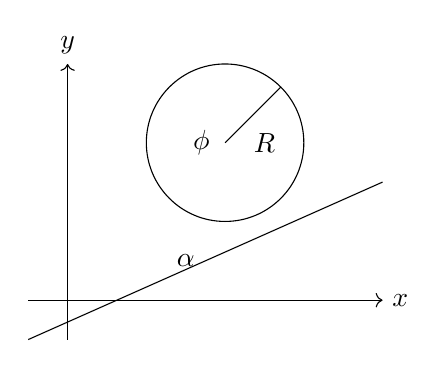
\begin{tikzpicture}
\draw[->] (-0.5,0) -- (4,0) node[right] {$x$};
\draw[->] (0,-0.5) -- (0,3) node[above] {$y$};
\draw (-0.5,-0.5) -- (4,1.5);
\draw (2,2) circle (1);
\draw (2,2) -- +(45:1);
\node at (1.5,0.5) {$\alpha$};
\node at (2.5,2) {$R$};
\node at (1.7,2) {$\phi$};
\end{tikzpicture}

Ohne ZBs würde die Lage der Scheibe durch 3 Koordinaten bestimmt,

ZB: $x_A, y_A, \phi$

2 holonome ZBs:

$x_A - R\phi \cos\alpha = 0$

$y_A - R\phi \sin\alpha = 0$
\end{EXA}

\begin{CONC}{CM-K25c-08-12}{Versionen der nicht-holonomen Zwangsbedingungen}
Nicht-holonome Zwangsbedingungen - Darunter versteht man alle ZB, die sich nicht auf Gleichungen der Form $f_j(q_1,...,q_M,t)=0$ zurückführen lassen, welche nur die generalisierten Koordinaten und die Zeit enthalten. (dabei ist M die maximal mögliche Zahl der generalisierten Koordinaten, $M=DN$ für N Teilchen in D Dimensionen).

Man unterscheidet zwei verschiedene Typen von nicht-holonomen ZB:

1) Ungleichungen:

Manche ZB lassen sich mathematisch nur als Ungleichungen formulieren.

\textbf{Beispiel:} Kleine Kugel rollt Oberfläche einer großen Kugel herunter:
ZB: $R(t) \geq R$

Ist die Geschwindigkeit der kleinen Kugel groß genug, verliert sie wegen ihrer Zentrifugalkraft beim Herunterfallen den Kontakt zur großen Kugel.

2) Nicht-integrable Zwangsbedingungen:

Darunter versteht man ZB der Form

\[f_j(q_1,...,q_M,\dot{q}_1,...,\dot{q}_M,t) = 0\]

die sich nicht durch geeignete Integration in holonome ZB der Form $h_j(q_1,...,q_M,t)=0$ umwandeln lassen.
\end{CONC}

\begin{CONC}{CM-K25c-08-13}{Holonomie und Exaktheit}
Betrachten wir zunächst eine \emph{holonome} Zwangsbedingung
\begin{equation}
  h_j\bigl(q_1,\dots,q_M,t\bigr)\;=\;0,
  \qquad j=1,\dots,k_{\mathrm{hol}} .
\end{equation}
Zeitliches Differenzieren liefert die (gleichwertige) Bedingung
\begin{equation}
  0 \;=\; \frac{\mathrm d}{\mathrm dt}\,
           h_j\bigl(q_1,\dots,q_M,t\bigr)
      \;=\;
      \sum_{i=1}^M 
        \frac{\partial h_j}{\partial q_i}\,\dot q_i
      + \frac{\partial h_j}{\partial t}
      \;\equiv\;
      f_j\bigl(\dot q_1,\dots,\dot q_M,t\bigr).
\end{equation}

% Differentialform
Multipliziert man mit $\mathrm dt$ und benutzt
$\mathrm dq_i = \dot q_i\,\mathrm dt$, erhält man die (Pfaffsche) 
Differentialform
\begin{equation}\label{eq:pfaff_hol}
  \sum_{i=1}^{M} a_{ji}\,\mathrm dq_i
  + a_{jt}\,\mathrm dt \;=\; 0, \qquad
  a_{ji}=\frac{\partial h_j}{\partial q_i},\quad
  a_{jt}=\frac{\partial h_j}{\partial t}.
\end{equation}

% Integrabilitätsbedingungen
Da die gemischten zweiten Ableitungen vertauschbar sind
(vorausgesetzt $h_j$ ist hinreichend glatt), gelten die
\emph{Integrabilitätsbedingungen}
\begin{align}
  \frac{\partial a_{ji}}{\partial q_k}
  &= \frac{\partial a_{jk}}{\partial q_i}
     \;=\;
     \frac{\partial^2 h_j}{\partial q_k\,\partial q_i},
     & i,k&=1,\dots,M,                                     \label{eq:int1}\\
  \frac{\partial a_{jt}}{\partial q_i}
  &= \frac{\partial a_{ji}}{\partial t}
     \;=\;
     \frac{\partial^2 h_j}{\partial q_i\,\partial t},
     & i&=1,\dots,M.                                       \label{eq:int2}
\end{align}
Die Pfaffsche Gleichung \eqref{eq:pfaff_hol} ist also \emph{exakt}, weil
sie als exaktes Differential $\mathrm d h_j$ entsteht.

% Nicht-integrable / nicht-holonome Zwangsbedingungen
In vielen Problemen treten jedoch \emph{nicht-holonome} (i.\,A.\, nicht
integrierbare) Zwangsbedingungen auf,
\begin{equation}\label{eq:pfaff_nh}
  \sum_{i=1}^{M} a_{ji}(q,t)\,\dot q_i
  + a_{jt}(q,t) \;=\; 0,
  \qquad j=1,\dots,k_{\mathrm{nh}},
\end{equation}
bzw.\ äquivalent in Differentialform
\(
  \sum_{i} a_{ji}\,\mathrm dq_i + a_{jt}\,\mathrm dt = 0 .
\)
Erfüllen die Koeffizienten $a_{ji},a_{jt}$ die
Integrabilitätsbedingungen \eqref{eq:int1}–\eqref{eq:int2} \emph{nicht},
so ist das Differential \emph{nicht exakt}.  

In manchen Fällen lässt sich durch Multiplikation mit einem
\emph{integrierenden Faktor} $\mu(q,t)\neq 0$
\[
  \mu\bigl(q,t\bigr)\,
  \Bigl(\sum_{i} a_{ji}\,\mathrm dq_i + a_{jt}\,\mathrm dt\Bigr)
  \;=\;
  \mathrm d H_j(q,t)
\]
eine exakte Form herstellen; gelingt dies jedoch nicht, kann
\eqref{eq:pfaff_nh} nicht auf eine holonome Bedingung
$H_j(q,t)=\text{const}$ integriert werden. Man spricht dann von einer
\emph{nicht-integrablen} Zwangsbedingung.
\end{CONC}

\begin{EXA}{CM-K25c-08-14}{Rollscheibe: Differentiale Zwangsbedingungen}
\textbf{1.\ Konfigurationskoordinaten}
Die Lage der Scheibe ist durch vier generalisierte Koordinaten vollständig
beschrieben
\[
  q \;=\; \bigl(x_A,\;y_A,\;\psi,\;\varphi\bigr)^{\mathrm T},
\]
\begin{itemize}
  \item $x_A,\;y_A$ – Koordinaten des Auflagepunktes $A$ in der Ebene,
  \item $\psi$ – Winkel zwischen der Bewegungsrichtung und der $x$-Achse,
  \item $\varphi$ – Rollwinkel der Scheibe um ihre Symmetrieachse.
\end{itemize}

\textbf{2.\ Kinematik des reinen Rollens}
Reines Abrollen ohne Gleiten liefert (Mechanik I, S.\,223)
\[
  V_{CM} \;=\; R\,\dot{\varphi},
\]
wobei die Geschwindigkeit des Schwerpunkts stets in die
Richtung $(\cos\psi,\,-\sin\psi)$ zeigt. Es folgt
\begin{align}
  \dot{x}_A &= R\,\dot{\varphi}\,\cos\psi,
  &
  \dot{y}_A &= -\,R\,\dot{\varphi}\,\sin\psi.
  \label{eq:velocities}
\end{align}

\textbf{3.\ Pfaffsche Zwangsbedingungen}
Die Geschwindigkeitsbeziehungen \eqref{eq:velocities} können als
differentiale (Pfaffsche) Zwangsbedingungen formuliert werden:
\begin{align}
  f_1 &:\; \boxed{\,dx_A - R\cos\psi\,d\varphi = 0\,},
  \label{eq:f1}\\[2mm]
  f_2 &:\; \boxed{\,dy_A + R\sin\psi\,d\varphi = 0\,}.
  \label{eq:f2}
\end{align}

\textbf{4.\ Integrabilitätsprüfung}

\paragraph{Zwangsbedingung \eqref{eq:f1}.}
Schreiben wir \eqref{eq:f1} als
\(
  \sum_{i=1}^{4} a_{1i}\,dq_i = 0
\)
mit den Koeffizienten
\[
  (a_{1x_A},\,a_{1y_A},\,a_{1\psi},\,a_{1\varphi})
  \;=\;
  (1,\,0,\,0,\,-R\cos\psi),
\]
so lautet die notwendige Integrabilitätsbedingung
\(
  \partial a_{1i}/\partial q_k
  =
  \partial a_{1k}/\partial q_i
\)
für alle Paare $(i,k)$.  
Für das Paar $(i,k)=(\psi,\varphi)$ ergibt sich
\[
  \frac{\partial a_{1\psi}}{\partial\varphi}
  \;=\; 0
  \;\neq\;
  \frac{\partial a_{1\varphi}}{\partial\psi}
  \;=\;
  R\sin\psi,
\]
womit \eqref{eq:f1} \emph{nicht integrierbar} ist.

\paragraph{Zwangsbedingung \eqref{eq:f2}.}
Für
\[
  (a_{2x_A},\,a_{2y_A},\,a_{2\psi},\,a_{2\varphi})
  \;=\;
  (0,\,1,\,0,\,R\sin\psi)
\]
liefert das Paar $(\psi,\varphi)$ den Widerspruch
\[
  \frac{\partial a_{2\psi}}{\partial\varphi}=0
  \;\neq\;
  \frac{\partial a_{2\varphi}}{\partial\psi}=R\cos\psi,
\]
sodass auch \eqref{eq:f2} nicht integrierbar ist.

\textbf{5.\ Kein integrierender Faktor für \eqref{eq:f1}}
Sei hypothetisch $\mu=\mu(q)\neq0$ so, dass $\mu\,f_1$ exakt wäre.
Notwendig wäre dann
\[
  \frac{\partial(\mu a_{1i})}{\partial q_k}
  \;=\;
  \frac{\partial(\mu a_{1k})}{\partial q_i}
  \quad\forall\,i,k.
\]
Aus dem Paar $(i,k)=(x_A,\psi)$ folgt
$\partial\mu/\partial\psi = 0$ (also $\mu$ unabhängig von $\psi$),
während das Paar $(\psi,\varphi)$ verlangt
\(
  \mu R\sin\psi = 0
\),
was bei beliebigem $\psi$ nur für $\mu\equiv0$ erfüllbar ist.
Ein nicht-trivialer integrierender Faktor existiert somit nicht.

\textbf{6.\ Schlussfolgerung}
Die Pfaffschen Gleichungen \eqref{eq:f1}–\eqref{eq:f2} verletzen die
Integrabilitätsbedingungen und besitzen keinen integrierenden Faktor.
Die Abrollbedingungen sind daher \emph{nicht holonom};
sie lassen sich nicht auf rein
koordinatenabhängige Gleichungen
\(
  H_j\bigl(x_A,y_A,\psi,\varphi\bigr)=\text{const.}
\)
zurückführen.
\end{EXA}

\begin{CONC}{CM-K25c-08-15}{Zwangkräfte in Newton'schen Bewegungsgleichungen}
\textbf*{Ziel}
Bestimmung der \emph{Zwangkräfte} (Reaktions- oder Führungskräfte) 
für \underline{holonome} Zwangsbedingungen innerhalb der klassisch
newton’schen Formulierung.

%--------------------------------------------------------------------
\textbf*{Gegeben}
\begin{itemize}
  \item $N$ Massenpunkte in $D$ Dimensionen $\;\Longrightarrow\; M=DN$
        kartesische Koordinaten\,(*)  
        \[
          \bigl\{\,x_{i}^{(\alpha)}\bigr\}_{\substack{i=1,\dots,N\\\alpha=1,\dots,D}},
          \quad
          \text{kurz } 
          (q_1,\dots,q_M).
        \]
  \item $k$ unabhängige \emph{holonome} Zwangsbedingungen
        \[
          f_j\bigl(q_1,\dots,q_M,t\bigr)=0,
          \qquad j=1,\dots,k .
        \]
\end{itemize}
Damit verbleiben $n=M-k$ unabhängige generalisierte Koordinaten.

%--------------------------------------------------------------------
\textbf*{Methode in drei Schritten}

\textbf{1.\ Wahl unabhängiger Koordinaten}
\[
  q_\mu = q_\mu(q_1,\dots,q_n,t), 
  \qquad \mu = 1,\dots,M .
\]
In kartesischer Form (hier $D=3$) erhält man
\[
  \vec r_i = 
  \begin{pmatrix}
    x_i(q_1,\dots,q_n,t)\\[2pt]
    y_i(q_1,\dots,q_n,t)\\[2pt]
    z_i(q_1,\dots,q_n,t)
  \end{pmatrix},
  \qquad
  i=1,\dots,N .
\]

\textbf{2.\ Newtonsche Bewegungsgleichungen}
\[
  m_i\,\ddot{\vec r}_i
  \;=\;
  \vec F_i^{\text{(ext)}}(q,\dot q,t)
  \;+\;
  \vec Z_i(q,\dot q,t),
  \qquad i=1,\dots,N .
\]
\emph{Unbekannt} sind hier die $M=DN$ Komponenten der
Zwangkräfte~$\vec Z_i$.

Sobald die Beschleunigungen $\ddot{\vec r}_i$
aus den Bewegungsgleichungen bestimmt sind, folgt
\[
  \vec Z_i 
  \;=\;
  m_i\,\ddot{\vec r}_i - \vec F_i^{\text{(ext)}} .
\]

\textbf{3.\ Eliminieren der Zwangkräfte}
\begin{itemize}
  \item Unbekannte Größen  
        \[
          \underbrace{q_1,\dots,q_{n}}_{\text{Koordinaten}}
          \quad\cup\quad
          \underbrace{Z_{1}^{(1)},\dots,Z_{N}^{(D)}}_{\text{Zwangkräfte}}
          \;\Longrightarrow\;
          (M-k)+M = 2M-k \text{ Unbekannte.}
        \]
  \item Gleichungen  
        \[
          \text{Newton: } M,\qquad
          \text{ZB + deren Zeitd.}: 2k
          \quad\Longrightarrow\quad
          M+2k \text{ Gleichungen.}
        \]
        Für holonome ZB ($k$ unabhängig) lassen sich $k$ der 
        $Z$-Komponenten rein algebraisch beseitigen, sodass exakt
        $M$ Gleichungen für die $M$ Unbekannten verbleiben.
  \item Ergebnis: Ein geschlossenes Differentialgleichungssystem
        \[
          \bigl\{\,q_\alpha(t)\bigr\}_{\alpha=1}^{n}
        \]
        ohne explizite Zwangkräfte.
\end{itemize}

\medskip
\noindent
(*) \emph{Indexkonvention:} $i$ zählt die Teilchen $(1,\dots,N)$,
$\alpha$ die kartesischen Komponenten $(1,\dots,D)$,
$q_1,\dots,q_M$ sind die vollständigen (u.\,U.\ abhängigen)
Koordinaten, $q_1,\dots,q_n$ die unabhängigen.
\end{CONC}

\begin{EXA}{CM-K25c-08-16}{Teilchen auf Kreiskegel}
\begin{center}
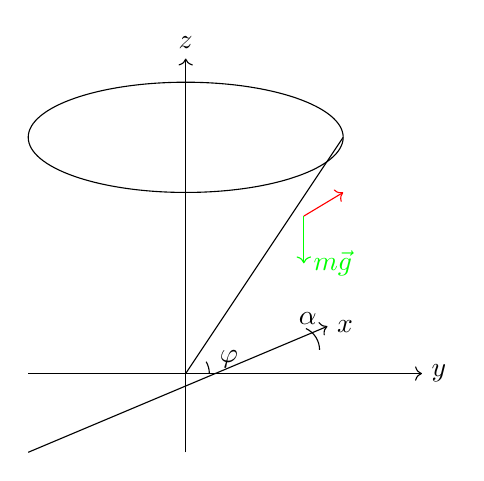
\begin{tikzpicture}[scale=1]
  % Achsen
  \draw[->] (-2,0) -- (3,0) node[right] {$y$};
  \draw[->] (0,-1) -- (0,4) node[above] {$z$};
  \draw[->] (-2,-1) -- (1.8,0.6) node[right] {$x$};
  % Kegel
  \draw (0,0) -- (2,3);
  \draw (0,3) ellipse (2cm and 0.7cm);
  \draw[dashed] (0,0) -- (2,0);
  % Winkel
  \draw (0.3,0) arc (0:30:0.3);
  \node at (0.55,0.18) {$\varphi$};
  \draw (1.7,0.3) arc (0:65:0.3);
  \node at (1.55,0.7) {$\alpha$};
  % Kräfte
  \draw[red,->] (1.5,2) -- (2,2.3);
  \draw[green,->] (1.5,2) -- (1.5,1.4) node[right] {$m\vec g$};
\end{tikzpicture}
\end{center}

\textbf{Geometrische Daten}\\
Ein Teilchen der Masse $m$ bewegt sich auf der Innenseite eines
Kreiskegels mit Halbwinkel $\alpha$ unter der Wirkung einer konstanten
Erdbeschleunigung $\vec g = -g\,\vec e_z$.  
Zylinderkoordinaten $(S,\varphi,z)$ sind geeignet; die
holonome Zwangsbedingung lautet
\[
  f(S,z)=S-z\tan\alpha=0
  \;\Longrightarrow\;
  z = S\cot\alpha .
\]

\textbf{Schritt 1 – unabhängige Koordinaten}\\
Wähle $q_1=S$ und $q_2=\varphi$.
Die kartesischen Orts­komponenten ergeben sich zu
\[
  \begin{pmatrix} x \\ y \\ z \end{pmatrix} =
  \begin{pmatrix}
    S\cos\varphi \\[2pt]
    S\sin\varphi \\[2pt]
    S\cot\alpha
  \end{pmatrix}.
\]

\textbf{Schritt 2 – Newtonsche Gleichungen mit Zwangkräften}\\
\[
  m\!
  \begin{pmatrix}
    \ddot x\\ \ddot y\\ \ddot z
  \end{pmatrix}
  =
  \underbrace{%
  \begin{pmatrix}
    0\\[2pt] 0\\[2pt] -\,mg
  \end{pmatrix}}_{\vec F^{\text{(ext)}}}
  +
  \underbrace{%
  \begin{pmatrix}
    Z_x\\ Z_y\\ Z_z
  \end{pmatrix}}_{\vec Z}.
\]
Mit
\[
  \dot x = \dot S\cos\varphi - S\dot\varphi\sin\varphi,\qquad
  \dot y = \dot S\sin\varphi + S\dot\varphi\cos\varphi,\qquad
  \dot z = \dot S\cot\alpha,
\]
folgen die Beschleunigungen
\begin{align}
  \ddot x &= \ddot S\cos\varphi - 2\dot S\dot\varphi\sin\varphi
             - S\dot\varphi^{2}\cos\varphi - S\ddot\varphi\sin\varphi,
             &(1)\nonumber\\[2pt]
  \ddot y &= \ddot S\sin\varphi + 2\dot S\dot\varphi\cos\varphi
             - S\dot\varphi^{2}\sin\varphi + S\ddot\varphi\cos\varphi,
             &(2)\nonumber\\[2pt]
  \ddot z &= \ddot S\cot\alpha. &(3)\nonumber
\end{align}
Damit lauten die Komponenten­gleichungen
\begin{align}
  m\bigl(\ddot S\cos\varphi - 2\dot S\dot\varphi\sin\varphi
        - S\dot\varphi^{2}\cos\varphi - S\ddot\varphi\sin\varphi\bigr) &= Z_x, \tag{A}\\[2pt]
  m\bigl(\ddot S\sin\varphi + 2\dot S\dot\varphi\cos\varphi
        - S\dot\varphi^{2}\sin\varphi + S\ddot\varphi\cos\varphi\bigr) &= Z_y, \tag{B}\\[2pt]
  m\bigl(\ddot S\cot\alpha\bigr) - mg &= -\,Z_z. \tag{C}
\end{align}
(Die Form \eqref{C} wählt $Z_z$ positiv nach oben.)

\textbf{Schritt 3 – Eliminieren der Zwangkräfte}\\
Die Reaktionskraft $\vec Z$ steht stets senkrecht zur Kegeloberfläche.  
Aus der Draufsicht (radiale Richtung)
\[
  \begin{pmatrix} Z_x\\ Z_y \end{pmatrix}
    = -\,Z_\perp\!\begin{pmatrix}\cos\varphi\\ \sin\varphi\end{pmatrix},
\]
folgt
\[
  Z_y\cos\varphi - Z_x\sin\varphi = 0. \tag{D}
\]
Aus der Seitenansicht (Neigungswinkel $\alpha$) erhält man
\[
  Z_z = Z_\perp\tan\alpha
  \;\Longrightarrow\;
  Z_z\cos\varphi + Z_x\tan\alpha = 0. \tag{E}
\]

\textbf{Kombination der Gleichungen}\\
\begin{enumerate}
  \item[(i)]  $(\text{A})\sin\varphi - (\text{B})\cos\varphi$
              unter Verwendung von \eqref{D} liefert
              \[
                2\dot S\,\dot\varphi + S\ddot\varphi = 0. \tag{1}
              \]
  \item[(ii)] $(\text{A})\tan\alpha + (\text{C})\cos\varphi$
              und Bedingung \eqref{E} ergeben
              \[
                (\tan\alpha + \cot\alpha)\,\ddot S
                - S\dot\varphi^{2}\tan\alpha + g = 0. \tag{2}
              \]
\end{enumerate}
Die zwei Differential­gleichungen \eqref{1} und \eqref{2} enthalten nur
die unabhängigen Koordinaten $S(t)$ und $\varphi(t)$;
die Zwangkräfte sind eliminiert.  
Nach Bestimmung von $S(t),\varphi(t)$ können $Z_x,Z_y,Z_z$ aus
(A)–(C) rückwärts berechnet werden.

\textbf{Fazit}\\
Das rein newton’sche Vorgehen erfordert
\emph{zuerst} das Einführen und
\emph{anschließende} Eliminieren der unbekannten Zwangkräfte – ein
umständlicher Prozess.  
Die Frage, ob man die Bewegungsgleichungen der unabhängigen Koordinaten
direkt (ohne $\vec Z$) erhält, wird von der Lagrange’schen Formulierung
beantwortet (D’Alembert–Lagrange-Prinzip).
\end{EXA}

\begin{CONC}{CM-K25c-09-01}{Alembert Prinzip}
Gegeben sei ein System aus $N$ Massenpunkten, auf die Zwangkräfte 
$\vec Z_i$ wirken.  
Nach dem d’Alembert-Prinzip verschwindet die Summe der von den 
$\vec Z_i$ verrichteten \emph{virtuellen} Arbeit:
\[
  \boxed{\;
    \delta W \;=\;\sum_{i=1}^{N}\vec Z_i\!\cdot\!\delta\vec r_i \;=\;0
  \;}
\]

\textbf{Virtuelle Verrückung $\delta\vec r_i$}
\begin{itemize}
  \item infinitesimal klein,
  \item verträglich mit allen Zwangsbedingungen,
  \item \emph{zeitlos} ($\delta t=0$): während $\delta\vec r_i$ werden 
        die ZB nicht verletzt.
\end{itemize}
\end{CONC}

\begin{REM}{CM-K25c-09-02}{Alembert Prinzip h d rheonomische ZB}
Bei zeitabhängigen (rheonomischen) ZB gilt zwar immer 
$\vec Z_i\!\cdot\!\delta\vec r_i=0$,  
doch die \emph{reale} Arbeit $\vec Z_i\!\cdot\!d\vec r_i$ kann ungleich 
Null sein.
\end{REM}

\begin{EXA}{CM-K25c-09-03}{Perle auf vertikal beschleunigten Draht}
\begin{center}
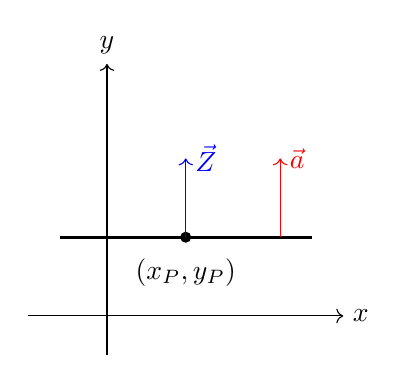
\begin{tikzpicture}[scale=1]
  \draw[->] (-1,0) -- (3,0) node[right] {$x$};
  \draw[->] (0,-0.5) -- (0,3.2) node[above] {$y$};
  \draw[very thick] (-0.6,1) -- (2.6,1);          % Draht
  \fill (1,1) circle (2pt);                       % Perle
  \node at (1,0.55) {$(x_P,y_P)$};
  \draw[blue,->] (1,1) -- (1,2) node[right] {$\vec Z$};
  \draw[red,->]  (2.2,1) -- (2.2,2) node[right] {$\vec a$};
\end{tikzpicture}
\end{center}

Zwangsbedingung (rheonom und holonom):
\[
  f(x_P,y_P,t) \;=\; y_P - \tfrac12 a t^{2} \;=\; 0 .
\]
Virtuelle Verrückungen erfüllen $\delta y_P = 0$, real hingegen 
$dy_P = a\,t\,dt \neq 0$:
\[
  \vec Z\!\cdot\!\delta\vec r_P = 0,
  \qquad
  \vec Z\!\cdot\!d\vec r_P = Z_y\,dy_P \neq 0.
\]
\end{EXA}

\begin{CONC}{CM-K25c-09-04}{Herleitung der d’Alembert-Gleichungen}
Aus den Newton’schen Gleichungen
\[
  m_i\ddot{\vec r}_i = \vec F_i + \vec Z_i,
  \qquad i=1,\dots,N,
\]
folgt nach Skalar­produkt mit $\delta\vec r_i$ und Summation:
\[
  \sum_{i=1}^{N}\bigl(m_i\ddot{\vec r}_i - \vec F_i\bigr)\!\cdot\!\delta\vec r_i
  = \sum_{i=1}^{N}\vec Z_i\!\cdot\!\delta\vec r_i = 0.
\]
Dies ist die \emph{d’Alembert-Gleichung}
\[
  \boxed{\;
    \sum_{i=1}^{N}\bigl(m_i\ddot{\vec r}_i - \vec F_i\bigr)
    \!\cdot\!\delta\vec r_i = 0
  \;}
\]
\end{CONC}

\begin{CONC}{CM-K25c-09-05}{Übergang zur Bewegungsgleichung für generelle Koordinaten}
Seien $k$ holonome ZB vorhanden ($n=M-k$ unabhängig).  
Schreibe
\[
  \vec r_i = \vec r_i(q_1,\dots,q_n,t)
  \quad\Longrightarrow\quad
  \delta\vec r_i = \sum_{j=1}^{n}
                   \frac{\partial\vec r_i}{\partial q_j}\,\delta q_j .
\]
Einsetzen in die d’Alembert-Gleichung liefert
\[
  \sum_{j=1}^{n}\!
  \Biggl[
    \sum_{i=1}^{N}
      \bigl(m_i\ddot{\vec r}_i - \vec F_i\bigr)
      \!\cdot\!
      \frac{\partial\vec r_i}{\partial q_j}
  \Biggr]\!
  \delta q_j = 0 .
\]
Da die $\delta q_j$ unabhängig sind, muss jede Klammer verschwinden:
\[
  \boxed{\;
    \sum_{i=1}^{N}\!
      \bigl(m_i\ddot{\vec r}_i - \vec F_i\bigr)
      \!\cdot\!
      \frac{\partial\vec r_i}{\partial q_j}
    = 0,
    \quad j=1,\dots,n.
  \;}
\]
Dies sind $n$ Bewegungsgleichungen für die unabhängigen Koordinaten 
$q_j$ – ohne explizite Zwangkräfte. Sie bilden den Ausgangspunkt der Lagrange’schen Formulierung.
\end{CONC}

\begin{EXA}{CM-K25c-09-06}{Teilchen auf Kreiskegel}
\textbf{d'Alembert-Gleichung}\\
\[
  (m\ddot{\vec r}-m\vec g)\!\cdot\!\delta\vec r = 0
  \;\Longleftrightarrow\;
  \ddot x\,\delta x + \ddot y\,\delta y + (\ddot z + g)\,\delta z = 0 .
\]

\textbf{Zwangsbedingung}\\
\[
  z = S\cot\alpha,
  \qquad\text{unabhängige Koordinaten: } S,\;\varphi .
\]

\textbf{Virtuelle Verrückungen}\\[-6pt]
\[
  \delta\vec r=
  \begin{pmatrix}
    \delta x\\ \delta y\\ \delta z
  \end{pmatrix}
  =
  \begin{pmatrix}
    \delta S\cos\varphi - S\sin\varphi\,\delta\varphi\\[2pt]
    \delta S\sin\varphi + S\cos\varphi\,\delta\varphi\\[2pt]
    \delta S\cot\alpha
  \end{pmatrix}.
\]

\textbf{Beschleunigungen in Zylinderkoordinaten}\\[-6pt]
\[
  \ddot{\vec r}=
  \begin{pmatrix}
    \ddot S\cos\varphi - 2\dot S\dot\varphi\sin\varphi
      - S\dot\varphi^{2}\cos\varphi - S\ddot\varphi\sin\varphi\\[2pt]
    \ddot S\sin\varphi + 2\dot S\dot\varphi\cos\varphi
      - S\dot\varphi^{2}\sin\varphi + S\ddot\varphi\cos\varphi\\[2pt]
    \ddot S\cot\alpha
  \end{pmatrix}.
\]

\textbf{Einsetzen in die d'Alembert-Gleichung}\\[-6pt]
\[
\begin{aligned}
  0 &=
  \ddot x\,\delta x + \ddot y\,\delta y + (\ddot z+g)\,\delta z \\[4pt]
    &=
  \bigl[\ddot x\cos\varphi+\ddot y\sin\varphi + (\ddot z+g)\cot\alpha\bigr]\delta S
  +\bigl[-\ddot x\sin\varphi + \ddot y\cos\varphi\bigr]S\,\delta\varphi \\[4pt]
    &=
  \bigl[(\tan\alpha+\cot\alpha)\ddot S
        - S\dot\varphi^{2}\tan\alpha + g\bigr]\cot\alpha\,\delta S
  +\bigl[2\dot S\dot\varphi + S\ddot\varphi\bigr]S\,\delta\varphi .
\end{aligned}
\]

\textbf{Unabhängigkeit der Variationen}\\
Wegen der Unabhängigkeit von $\delta S$ und $\delta\varphi$ müssen die
Klammern einzeln verschwinden:
\[
  \boxed{
  \begin{aligned}
    2\dot S\,\dot\varphi + S\,\ddot\varphi &= 0,\\[2pt]
    (\tan\alpha+\cot\alpha)\ddot S
      - S\dot\varphi^{2}\tan\alpha + g &= 0.
  \end{aligned}}
\]
Damit erhält man dieselben Bewegungsgleichungen wie zuvor, jedoch ohne
explizite Bestimmung der Zwangkräfte.
\end{EXA}

\begin{CONC}{CM-K25c-09-07}{Rezept: Bewegungsgleichungen aus der d’Alembert-Gleichung}
\textbf{Vorgehen}\\[-4pt]
\begin{enumerate}
  \item Schreibe die d’Alembert-Gleichung in kartesischen Koordinaten
        \[
          \sum_{i=1}^{N}
            \bigl(m_i\ddot{\vec r}_i-\vec F_i\bigr)\!\cdot\!\delta\vec r_i = 0 .
        \]
  \item Drücke alle kartesischen Koordinaten $\vec r_i$ mittels der
        unabhängigen generalisierten Koordinaten
        $q_1,\dots,q_n$ (und ggf.\ $t$) aus; ersetze entsprechend
        $\delta\vec r_i$.
  \item Setze die (linear unabhängigen) Koeffizienten der Variationen
        $\delta q_j$ gleich Null.  
        Dies liefert $n$ Bewegungsgleichungen für
        $q_1(t),\dots,q_n(t)$ ohne explizite Zwangkräfte.
\end{enumerate}
\end{CONC}

\begin{CONC}{CM-K25c-09-08}{Gleichgewichtsprinzip}
Im statischen Gleichgewicht gilt $\ddot{\vec r}_i=0$. Die d’Alembert-Gleichung reduziert sich auf
\[
  \sum_{i=1}^{N}\vec F_i\!\cdot\!\delta\vec r_i = 0 .
\]
Damit verschwindet die virtuelle Arbeit aller äußeren Kräfte
im Gleichgewicht.
\end{CONC}

\begin{CONC}{CM-K25c-09-09}{Bestimmung von Zwangkräften über ein virtuelles Zusatz­system}
Soll eine bestimmte Zwangkraft $\vec Z^{\ast}$ berechnet werden, behandelt man sie gedanklich als
\emph{eingeprägte} (äußere) Kraft; die zugehörige ZB ist damit vorübergehend aufgehoben. Das System erhält dadurch einen zusätzlichen Freiheitsgrad. Die d’Alembert-Gleichung liefert nun eine weitere Bedingung, aus der $\vec Z^{\ast}$ (als unbekannte eingeprägte Kraft) algebraisch bestimmt werden kann. Auf diese Weise lässt sich die gesuchte Zwangkraft ermitteln, ohne alle anderen Reaktionskräfte explizit zu kennen.
\end{CONC}

\begin{EXA}{CM-K25c-09-10}{Leiter an Wand im Gleichgewicht}
\textbf{Geometrie und Kräfte}

\begin{itemize}
\item Leiter: Länge $L$, Masse $M$, Schwerpunkt $S$ in der Mitte
      \[
        (x_S,y_S)=\Bigl(\tfrac{L}{2}\cos\alpha,\;\tfrac{L}{2}\sin\alpha\Bigr).
      \]
\item Mensch: Masse $m$, steht im Abstand\footnote{%
      $\ell$ ist die Weglänge entlang der Leiter von der Spitze
      \emph{B} abwärts.}  
      $\ell$ von der Leiter­spitze B
      \[
        (x_B,y_B)=\bigl((L-\ell)\cos\alpha,\;\ell\sin\alpha\bigr).
      \]
\item Auflagepunkt der Leiter auf dem Boden A
      \[
        (x_A,y_A)=\bigl(L\cos\alpha,\,0\bigr).
      \]
\item Eingeprägte Kräfte: 
      $M\vec g$ am Schwerpunkt $S$,  
      $m\vec g$ am Punkt $B$  
      ($\vec g=-g\,\vec e_y$).
\item Gesuchte Größe: horizontale Seil- bzw.\ Stütz­kraft
      $\vec F = F\,\vec e_x$ am Punkt A.
\end{itemize}

%--------------------------------------------------------------
%  \textbf{Virtuelle Arbeit (Gleichgewichtsprinzip)}
%--------------------------------------------------------------
Da sich das System im Gleichgewicht befindet ($\ddot{\vec r}=0$),
verschwindet die Summe der virtuellen Arbeiten:
\[
  -\,Mg\,\delta y_S
  -\,mg\,\delta y_B
  -\,F\,\delta x_A
  \;=\;0 .
\]

%--------------------------------------------------------------
%  \textbf{Variation mittels des einzigen Freiheitsgrads $\alpha$}
%--------------------------------------------------------------
\[
\begin{aligned}
  \delta x_A &= -L\sin\alpha\,\delta\alpha,\\
  \delta y_S &= \tfrac{L}{2}\cos\alpha\,\delta\alpha,\\
  \delta y_B &= \ell\cos\alpha\,\delta\alpha.
\end{aligned}
\]

Einsetzen in das Gleichgewichtsprinzip ergibt
\[
  \bigl(
    -\,Mg\,\tfrac{L}{2}\cos\alpha
    -\,mg\,\ell\cos\alpha
    +\,F\,L\sin\alpha
  \bigr)\,\delta\alpha = 0.
\]

%--------------------------------------------------------------
%  \textbf{Lösung für $F$}
%--------------------------------------------------------------
Da $\delta\alpha$ beliebig ist,
\[
  F
  \;=\;
  g\,\cot\alpha
  \Bigl(\tfrac{M}{2} + m\,\tfrac{\ell}{L}\Bigr).
\]

\textbf{Interpretation}

\begin{itemize}
\item $F$ wächst, wenn der Mensch höher steigt
      ($\ell\!\uparrow\Rightarrow y_B\uparrow$).
\item Für eine steilere Leiter ($\alpha\!\uparrow$)
      nimmt $F$ proportional zu $\cot\alpha$ ab.
\item Setzt man $m=0$ (kein Mensch), bleibt nur der Term
      $Mg/2$ – die Hälfte des Leitergewichts wirkt in die Seil­spannung
      ein.
\end{itemize}
\end{EXA}

\begin{CONC}{CM-K25c-09-11}{Zwangkräfte als Normalenkräfte und Ursprung des d’Alembert-Prinzips}
\textbf{Erfahrungstatsache}\\
Für einen Massenpunkt, dessen Bewegung durch eine \emph{holonome}
Zwangsbedingung
\[
  f\!\bigl(\vec r,t\bigr)=0
\]
eingeschränkt ist, gilt empirisch
\[
  \boxed{\;
    \vec Z = m\ddot{\vec r}-\vec F
    = \lambda(\vec r,\dot{\vec r},t)\,
      \nabla_{\!\vec r} f(\vec r,t)
  \;}
\]
mit einem skalar-wertigen Lagrange-Multiplikator $\lambda$.  
Da $\nabla_{\!\vec r}f$ senkrecht auf der Fläche $f=\text{const}$
steht, wirkt die Zwangkraft \emph{normal} auf die Bahnfläche.

\textbf{Folgerung}\\
Virtuelle Verrückungen $\delta\vec r$ sind tangential zur
Bahnfläche und erfüllen
\[
  \nabla_{\!\vec r} f\!\cdot\!\delta\vec r = 0
  \;\;\Longrightarrow\;\;
  \vec Z\!\cdot\!\delta\vec r
  = \lambda\,\nabla_{\!\vec r}f\!\cdot\!\delta\vec r = 0 .
\]
Damit folgt unmittelbar das d’Alembert-Prinzip
$\sum\vec Z_i\!\cdot\!\delta\vec r_i = 0$.
\end{CONC}

\begin{EXA}{CM-K25c-09-12}{Block auf einer schiefen Ebene}
\textbf{Zwangsbedingung und Gradient}\\
Für eine Ebene mit Steigungswinkel $d$ sei
\[
  f(\vec r) = Y - X\tan d = 0
  \quad\Longrightarrow\quad
  \nabla_{\!\vec r}f
  = -\tan d\,\vec e_x + \vec e_y .
\]

\textbf{Zwangkraft}\\
Nach der Erfahrungstatsache
\[
  \vec Z
  = \lambda\,\bigl(-\tan d\,\vec e_x + \vec e_y\bigr),
\]
also senkrecht zur Gleitfläche.  
Virtuelle Verrückungen auf der Ebene erfüllen
$\delta Y = \tan d\,\delta X$ und sind daher orthogonal zu
$\nabla_{\!\vec r}f$:
\[
  \vec Z\!\cdot\!\delta\vec r
  = \lambda\,(-\tan d\,\delta X + \delta Y) = 0 .
\]
Damit ist die virtuelle Arbeit der Zwangkraft null; 
das d’Alembert-Prinzip ist hiermit veranschaulicht.
\end{EXA}

\begin{CONC}{CM-K25c-09-13}{Verallgemeinerung auf $N$ Teilchen und $k$ Zwangsbedingungen}
\textbf{a) Holonome Zwangsbedingungen}\\
Sind $k$ unabhängige, holonome Bedingungen
\[
  f_j\!\bigl(\vec r_1,\dots,\vec r_N,t\bigr)=0,
  \qquad j=1,\dots,k
\]
gegeben, so hat jede Zwangskraft die Gestalt
\[
  \boxed{\,%
    \vec Z_i =
    \sum_{j=1}^{k}
      \lambda_j(\vec r_1,\dots,\vec r_N,
                \dot{\vec r}_1,\dots,\dot{\vec r}_N,t)\,
      \nabla_{\!\vec r_i} f_j(\vec r_1,\dots,\vec r_N,t)
    \,}, \qquad i=1,\dots,N.
\]
Setzt man
\[
  \vec a_{ji}(\vec r_1,\dots,\vec r_N,t)
  :=\nabla_{\!\vec r_i} f_j(\vec r_1,\dots,\vec r_N,t),
\]
so lautet dieselbe Beziehung kurz
\[
  \vec Z_i = \sum_{j=1}^{k}\lambda_j\,\vec a_{ji}.
\]
Für Punktmassen in allgemeinen Koordinaten
\(
  q_1,\dots,q_M
\)
erscheint $\vec a_{ji}$ als
\(
  a_{ji}=\partial h_j/\partial q_i
\)
(vgl.\ Kap.~2.1\,c).

\textbf{b) Differential-Zwangsbedingungen}\\
Liegen die $k$ Bedingungen nur in Pfaffscher Form vor
\[
  \sum_{i=1}^{N}\vec a_{ji}\!\cdot d\vec r_i + a_{jt}\,dt = 0,
  \qquad j=1,\dots,k,
\]
so gilt analog
\[
  \boxed{\,%
    \vec Z_i = \sum_{j=1}^{k}\lambda_j\,\vec a_{ji},
    \qquad i=1,\dots,N.%
  \,}
\]
\end{CONC}

\begin{CONC}{CM-K25c-09-14}{Verallgemeinerung auf $N$ Teilchen Herleitung der AP}
\textbf{Virtuelle Verrückungen}\\
Für eine holonome Bedingung folgt
\[
  0 = \delta f_j
    = \sum_{i=1}^{N}\nabla_{\!\vec r_i}f_j\!\cdot\!\delta\vec r_i
    = \sum_{i=1}^{N}\vec a_{ji}\!\cdot\!\delta\vec r_i,
\]
und bei Pfaffschen ZB gilt wegen $\delta t=0$ dasselbe Resultat.

\textbf{Virtuelle Arbeit der Zwangkräfte}\\
\[
  \sum_{i=1}^{N}\vec Z_i\!\cdot\!\delta\vec r_i
  = \sum_{i=1}^{N}
      \Bigl(\sum_{j=1}^{k}\lambda_j\,\vec a_{ji}\Bigr)
      \!\cdot\!\delta\vec r_i
  = \sum_{j=1}^{k}\lambda_j
      \Bigl(\sum_{i=1}^{N}\vec a_{ji}\!\cdot\!\delta\vec r_i\Bigr)
  = 0.
\]
Damit ergibt sich unmittelbar das \emph{d’Alembert-Prinzip}
\[
  \boxed{\;
    \sum_{i=1}^{N}\vec Z_i\!\cdot\!\delta\vec r_i = 0
  \;}
\]
als Konsequenz der Tatsache, dass Zwangkräfte stets normal auf
den vom System einzuhaltenden Zwangsflächen bzw.\ -bahnen stehen.
\end{CONC}

\begin{CONC}{CM-K25c-09-15}{Übersicht zentraler Sätze des Lagrange Formalismus}
\begin{enumerate}
  \item \textbf{d’Alembert-Prinzip}  
        \[
          \boxed{\;
            \sum_{i=1}^{N} \vec Z_i \!\cdot\! \delta\vec r_i = 0
          \;}
        \]
        Die gesamte virtuelle Arbeit der Zwangkräfte verschwindet.

  \item \textbf{d’Alembert-Gleichung}  
        \[
          \boxed{\;
            \sum_{i=1}^{N}
              \bigl(m_i\ddot{\vec r}_i - \vec F_i\bigr)
              \!\cdot\! \delta\vec r_i = 0
          \;}
        \]
        Durch Einbeziehen der Trägheitskräfte wird die Wirkung der
        Zwangkräfte eliminiert.

  \item \textbf{Bewegungsgleichungen in unabhängigen
        Koordinaten\,$q_1,\dots,q_n$}  
        Bei $k$ holonomen Bedingungen ($n=M-k$):
        \[
          \boxed{\;
            \sum_{i=1}^{N}
              \bigl(m_i\ddot{\vec r}_i - \vec F_i\bigr)
              \!\cdot\!
              \frac{\partial\vec r_i}{\partial q_j}
            = 0,
            \quad j=1,\dots,n
          \;}
        \]
        Dies sind $n$ Differentialgleichungen ohne explizite
        Zwangkräfte.

  \item \textbf{Gleichgewichtsprinzip}  
        \[
          \boxed{\;
            \sum_{i=1}^{N} \vec F_i \!\cdot\! \delta\vec r_i = 0
          \;}
        \]
        Im statischen Gleichgewicht (\,${\ddot{\vec r}}_i=0$\,) leistet
        die Gesamtheit der eingeprägten Kräfte keine virtuelle Arbeit.
\end{enumerate}
\end{CONC}

\section{Lagrange}

\subsection{Lagrange 2}

\begin{CONC}{CM-K25c-10-01}{Herleitung der Lagrange-Gleichungen 2. Art aus der d’Alembert-Gleichung}
\textbf{1.\ Ausgangspunkt: d’Alembert-Gleichung}

\[
  \sum_{i=1}^{N}\bigl(m_i\ddot{\vec r}_i-\vec F_i\bigr)\!\cdot\!\delta\vec r_i=0.
\]

\textbf{2.\ Verallgemeinerte Koordinaten}

Wähle $n$ (später unabhängige) Koordinaten $q_1,\dots,q_n$  
und setze
\[
  \vec r_i=\vec r_i(q_1,\dots,q_n,t),
  \qquad
  \delta\vec r_i=\sum_{j=1}^{n}
                  \frac{\partial\vec r_i}{\partial q_j}\,\delta q_j.
\]

\textbf{3.\ Generalisierte Kräfte}

\[
  \sum_{i=1}^{N}\vec F_i\!\cdot\!\delta\vec r_i
  =\sum_{j=1}^{n}
     \underbrace{\Bigl(
       \sum_{i=1}^{N}\vec F_i\!\cdot\!
       \frac{\partial\vec r_i}{\partial q_j}
     \Bigr)}_{=:\,Q_j}
     \delta q_j.
\]

\textbf{4.\ Transformation des Trägheitsterms}

\[
\begin{aligned}
  \sum_{i=1}^{N}m_i\ddot{\vec r}_i\!\cdot\!\delta\vec r_i
  &=\sum_{j=1}^{n}\!
     \Bigl[
       \sum_{i=1}^{N}
         m_i\ddot{\vec r}_i\!\cdot\!
         \frac{\partial\vec r_i}{\partial q_j}
     \Bigr]\delta q_j\\[2pt]
  &=\sum_{j=1}^{n}\!
     \Bigl[
       \frac{\mathrm d}{\mathrm dt}
         \Bigl(
           \sum_{i=1}^{N}
             m_i\dot{\vec r}_i\!\cdot\!
             \frac{\partial\vec r_i}{\partial q_j}
         \Bigr)
       -
       \sum_{i=1}^{N}
         m_i\dot{\vec r}_i\!\cdot\!
         \frac{\mathrm d}{\mathrm dt}
           \frac{\partial\vec r_i}{\partial q_j}
     \Bigr]\delta q_j .
\end{aligned}
\]

Da
\(
  \dfrac{\mathrm d}{\mathrm dt}
  \dfrac{\partial\vec r_i}{\partial q_j}
  =
  \dfrac{\partial\dot{\vec r}_i}{\partial q_j},
\)
ergibt sich mit
\(
  T=\sum_{i=1}^{N}\tfrac12m_i\dot{\vec r}_i^{\,2}
\)

\[
  \sum_{i=1}^{N}m_i\ddot{\vec r}_i\!\cdot\!\delta\vec r_i
  =
  \sum_{j=1}^{n}
    \Bigl[
      \frac{\mathrm d}{\mathrm dt}
        \Bigl(\frac{\partial T}{\partial\dot q_j}\Bigr)
      -
      \frac{\partial T}{\partial q_j}
    \Bigr]\delta q_j .
\]

\textbf{5.\ d’Alembert–Lagrange-Gleichung}

Einsetzen in die d’Alembert-Gleichung liefert

\[
  \sum_{j=1}^{n}
    \Bigl[
      \frac{\mathrm d}{\mathrm dt}\frac{\partial T}{\partial\dot q_j}
      -
      \frac{\partial T}{\partial q_j}
      -
      Q_j
    \Bigr]\delta q_j=0.
\]

Bei $k$ holonomen ZB sind $n=3N-k$ Koordinaten unabhängig, also

\[
  \boxed{\;
    \frac{\mathrm d}{\mathrm dt}\frac{\partial T}{\partial\dot q_j}
    -
    \frac{\partial T}{\partial q_j}
    =Q_j,
    \qquad j=1,\dots,n .\;}
\]

\textbf{6.\ Einführung eines (generalisierten) Potentials}

\begin{itemize}
\item \textbf{Konservative Kräfte}  
      $\vec F_i=-\nabla_{\vec r_i}V(\vec r_1,\dots,\vec r_N,t)$  
      $\Longrightarrow\;Q_j=-\dfrac{\partial V}{\partial q_j}$.
\item \textbf{Geschwindigkeitsabhängige Kräfte}  
      Existiert ein \emph{generalisiertes Potential}
      $V(q,\dot q,t)$ mit
      \[
        Q_j=-\frac{\partial V}{\partial q_j}
            +\frac{\mathrm d}{\mathrm dt}
             \frac{\partial V}{\partial\dot q_j},
      \]
      dann bleibt die Struktur erhalten.
\end{itemize}

\textbf{7.\ Lagrange-Funktion und Gleichungen 2.\ Art}

Definiere
\[
  L(q,\dot q,t)=T(q,\dot q,t)-V(q,\dot q,t).
\]
Dann wird die letzte Gleichung zu

\[
  \boxed{\;
    \frac{\mathrm d}{\mathrm dt}\frac{\partial L}{\partial\dot q_j}
    -
    \frac{\partial L}{\partial q_j}=0,
    \qquad j=1,\dots,n
  \;}
\]

– den \emph{Lagrange-Gleichungen 2.\ Art}.  
Sie gelten genau dann, wenn
\begin{itemize}
  \item die Zwangbedingungen holonom sind und
  \item alle eingeprägten Kräfte aus einem (möglicherweise
        geschwindigkeitsabhängigen) Potential stammen.
\end{itemize}
\end{CONC}

\begin{EXA}{CM-K25c-10-02}{Elektromagnetische Kraft auf Teilchen mit Ladung}
Elektromagnetische Kraft auf Teilchen der Ladung $Q$ (Lorentz-Kraft, siehe Elektrodynamik)

Das generalisierte Potential für ein geladenes Teilchen im elektromagnetischen Feld lautet:
\[
V(\vec{r}, \dot{\vec{r}}) = Q \left( \phi(\vec{r}) - \frac{1}{c} \dot{\vec{r}} \cdot \vec{A}(\vec{r}) \right),
\]
mit zugehöriger Kraft:
\[
\vec{F} = Q \left( \vec{E} + \frac{1}{c} \dot{\vec{r}} \times \vec{B} \right),
\]
wobei die Felder durch
\[
\vec{E} = -\vec{\nabla} \phi - \frac{1}{c} \frac{\partial \vec{A}}{\partial t}, 
\quad 
\vec{B} = \vec{\nabla} \times \vec{A}
\]
gegeben sind.

\vspace{1em}
\end{EXA}

\begin{EXA}{CM-K25c-10-03}{Teilchen auf der Innenseite eines Kreiskegels (Lagrange-Formulierung)}
\textbf{Geometrie und Zwangsbedingung}\\
Zylinderkoordinaten $(\rho,\varphi,z)$ mit der holonomen Bedingung  
\[
  f(\rho,z)=\rho-z\tan\alpha=0
  \;\;\Longrightarrow\;\;
  z=\rho\cot\alpha .
\]
Als unabhängige generalisierte Koordinaten wählen wir
\[
  q_1=\rho\;(\equiv s), 
  \qquad 
  q_2=\varphi .
\]

\textbf{1.\ Lagrange-Funktion}\\
Die kartesische Geschwindigkeit lautet
\(
  \dot{\vec r}^{\,2}=\dot\rho^{2}+\rho^{2}\dot\varphi^{2}+\dot z^{2}.
\)
Unter Berücksichtigung der ZB ($\dot z=\cot\alpha\,\dot\rho$) ergibt sich  
\[
  T=\frac{m}{2}\!\bigl(\dot\rho^{2}+\rho^{2}\dot\varphi^{2}
        +\cot^{2}\!\alpha\,\dot\rho^{2}\bigr)
    =\frac{m}{2}\!\bigl((1+\cot^{2}\!\alpha)\dot\rho^{2}
        +\rho^{2}\dot\varphi^{2}\bigr).
\]
Das Potential ist $V=m g z=m g\rho\cot\alpha$.  
Damit
\[
  L(\rho,\dot\rho,\varphi,\dot\varphi)
  =T-V
  =\frac{m}{2}\!\bigl((1+\cot^{2}\!\alpha)\dot\rho^{2}
        +\rho^{2}\dot\varphi^{2}\bigr)
   -mg\rho\cot\alpha .
\]

\textbf{2.\ Lagrange-Gleichungen}\\[-6pt]
\[
\boxed{
  \begin{aligned}
    &\frac{\mathrm d}{\mathrm dt}
       \Bigl((1+\cot^{2}\!\alpha)\,m\dot\rho\Bigr)
      -\Bigl(m\rho\dot\varphi^{2}-mg\cot\alpha\Bigr)=0,\\[4pt]
    &\frac{\mathrm d}{\mathrm dt}\bigl(m\rho^{2}\dot\varphi\bigr)=0.
  \end{aligned}}
\]
\textit{kompakt}
\[
  (1+\cot^{2}\!\alpha)\,\ddot\rho-\rho\dot\varphi^{2}
  +g\cot\alpha=0,
  \qquad
  2\dot\rho\,\dot\varphi+\rho\,\ddot\varphi=0.
\]

\textbf{3.\ Konsistenz}\\
Die Gleichungen stimmen (nach Umformung mit  
$\cot\alpha=\tfrac{1}{\tan\alpha}$) mit den Resultaten 
\[
  (\tan\alpha+\cot\alpha)\ddot\rho-\rho\dot\varphi^{2}\tan\alpha+g=0,
  \qquad
  2\dot\rho\,\dot\varphi+\rho\,\ddot\varphi=0
\]
aus Kap.\,2.2 (S.\,33) überein.  
Der Lagrange-Formalismus liefert somit dieselben Bewegungsgleichungen, 
ohne dass Zwangkräfte explizit auftreten.
\end{EXA}

\begin{CONC}{CM-K25c-10-04}{Forminvarianz der Lagrangegleichungen unter Punkttransformation}
%--------------------------------------------------------------------
\textbf{Forminvarianz der Lagrange-Gleichungen}
%--------------------------------------------------------------------

Gegeben sei eine Lagrange-Funktion
\[
  L(q_1,\dots,q_n,\dot q_1,\dots,\dot q_n,t),
  \qquad
  n = 3N-k ,
\]
für die bereits gilt
\[
  \boxed{%
    \frac{\mathrm d}{\mathrm dt}\frac{\partial L}{\partial\dot q_j}
    -\frac{\partial L}{\partial q_j}=0,
    \quad j=1,\dots,n }.
\]

\textbf{Punkttransformation}\\
Wir führen eine reguläre (d.\,h. invertierbare) Punkttransformation ein  
\[
  q'_j = q'_j(q_1,\dots,q_n,t),
  \qquad
  (J:=\det{\partial q'_j/\partial q_i}\neq0),
\]
mit der Inversen
\( q_i = q_i(q'_1,\dots,q'_n,t) \).
Die neuen Geschwindigkeiten sind
\[
  \dot q_i(q',\dot q',t)
  =\sum_{k=1}^{n}\frac{\partial q_i}{\partial q'_k}\,\dot q'_k
   +\frac{\partial q_i}{\partial t}.
\]

\textbf{Transformation der Lagrange-Funktion}\\
\[
  \boxed{%
    L'(q',\dot q',t)
    =L\!\bigl(q(q',t),\dot q(q',\dot q',t),t\bigr)}.
\]
$L'$ ist also ein \emph{Skalar}: sein numerischer Wert bleibt erhalten,
nur die Darstellung in den Koordinaten ändert sich.

%--------------------------------------------------------------------
\textbf{Ableitungen von $L'$}
%--------------------------------------------------------------------
\[
  \frac{\partial L'}{\partial q'_j}
  =\sum_{i=1}^{n}\Bigl(
      \frac{\partial L}{\partial q_i}\,
      \frac{\partial q_i}{\partial q'_j}
     +\frac{\partial L}{\partial\dot q_i}\,
      \frac{\partial\dot q_i}{\partial q'_j}\Bigr),\qquad
  \frac{\partial L'}{\partial\dot q'_j}
  =\sum_{i=1}^{n}
      \frac{\partial L}{\partial\dot q_i}\,
      \frac{\partial q_i}{\partial q'_j}.
\]
Dabei wurden die elementaren Beziehungen
\[
  \boxed{%
    \frac{\partial\dot q_i}{\partial\dot q'_j}=
    \frac{\partial q_i}{\partial q'_j}},
  \qquad
  \boxed{%
    \frac{\mathrm d}{\mathrm dt}
    \Bigl(\frac{\partial q_i}{\partial q'_j}\Bigr)=
    \frac{\partial\dot q_i}{\partial q'_j}}
\]
genutzt (direkte Ableitung und Vertauschung der partiellen Differentiationen).

%--------------------------------------------------------------------
\textbf{Lagrange-Gleichungen in den neuen Koordinaten}
%--------------------------------------------------------------------
\[
\begin{aligned}
  \frac{\mathrm d}{\mathrm dt}
    \Bigl(\frac{\partial L'}{\partial\dot q'_j}\Bigr)
  -\frac{\partial L'}{\partial q'_j}
  &=
  \sum_{i=1}^{n}
    \Bigl[\,
      \frac{\mathrm d}{\mathrm dt}
        \Bigl(\frac{\partial L}{\partial\dot q_i}\Bigr)
      -\frac{\partial L}{\partial q_i}\Bigr]
    \frac{\partial q_i}{\partial q'_j}\;=\;0 .
\end{aligned}
\]
Der letzte Schritt folgt, weil der Klammerausdruck für jedes
$i$ aufgrund der ursprünglichen Lagrange-Gleichungen verschwindet.
Damit ist bewiesen:

\[
  \boxed{%
    \frac{\mathrm d}{\mathrm dt}
      \frac{\partial L'}{\partial\dot q'_j}
    -\frac{\partial L'}{\partial q'_j}=0,
    \quad j=1,\dots,n }.
\]

%--------------------------------------------------------------------
\textbf{Ergebnis}
%--------------------------------------------------------------------
Die Lagrange-Gleichungen sind \emph{forminvariant} unter beliebigen
regulären Punkttransformationen
\( q\mapsto q'(q,t) \).
Insbesondere behalten sie ihre Gestalt auch in beschleunigten
(Bezugs-) Koordinatensystemen.
\end{CONC}

\begin{EXA}{CM-K25c-10-05}{Freies Teilchen in einer Dimension im beschleunigten Bezugssystem}
Die Lagrangefunktion im Inertialsystem lautet:
\[
L(x,\dot{x},t) = T(\dot{x}) = \frac{1}{2} m \dot{x}^2
\]
Die Lagrange-Gleichung ergibt:
\[
\frac{d}{dt} \frac{\partial L}{\partial \dot{x}} - \frac{\partial L}{\partial x} = m \ddot{x} = 0
\]
Wir betrachten nun ein Bezugssystem, das sich entlang der \( x \)-Achse mit zeitabhängiger Beschleunigung \( A(t) \) bewegt:

\begin{center}
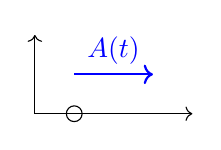
\begin{tikzpicture}
\draw[->] (0,0) -- (2,0);
\draw[->] (0,0) -- (0,1);
\draw[blue,->, thick] (0.5,0.5) -- (1.5,0.5);
\draw (0.5,0) circle (0.1);
\node[blue] at (1,0.8) {$A(t)$};
\end{tikzpicture}
\end{center}

Der Zusammenhang zwischen den Koordinaten ist:
\[
x' = x - \int_0^t V(t') \, dt', 
\quad \text{mit} \quad A(t) = \frac{dV}{dt}
\]
Daraus folgt für die Geschwindigkeiten:
\[
\dot{x}' = \dot{x} - V(t), 
\quad \Rightarrow \dot{x} = \dot{x}' + V(t)
\]
Einsetzen in die ursprüngliche Lagrangefunktion ergibt die transformierte Lagrangefunktion im beschleunigten System:
\[
L'(x', \dot{x}', t) = L(x(x', t), \dot{x}(x', \dot{x}', t), t) = \frac{m}{2}(\dot{x}' + V(t))^2
\]
Anwenden der Lagrange-Gleichung im beschleunigten System:
\[
\frac{d}{dt} \left( \frac{\partial L'}{\partial \dot{x}'} \right) - \frac{\partial L'}{\partial x'} 
= \frac{d}{dt} \left( m (\dot{x}' + V(t)) \right) = m (\ddot{x}' + A(t)) = 0
\]
Daraus folgt:
\[
m \ddot{x}' = -m A(t)
\]

\noindent\textbf{Interpretation:}  
Die Scheinkraft \( -mA(t) \) tritt ganz natürlich in der Lagrange-Gleichung auf – sie ist eine direkte Folge der Transformation in ein beschleunigtes Bezugssystem.  
\\[1ex]
\textit{Die in beschleunigten Bezugssystemen auftretenden Scheinkräfte sind also automatisch in den Lagrange-Gleichungen enthalten!}
\end{EXA}

\begin{CONC}{CM-K25c-10-06}{Symmetrien Invarianzen Erhaltungsgrößen}
\begin{enumerate}

%--------------------------------------------------------------
\item \textbf{Symmetrie}  
Ein mechanisches System ist \emph{symmetrisch} gegenüber einer
Operation, wenn sich sein beobachtbarer Zustand nach Ausführung der
Operation nicht ändert.

\textit{Beispiel:} Eine perfekte Kugel bleibt unter beliebiger
Drehung um ihren Mittelpunkt unverändert.

%--------------------------------------------------------------
\item \textbf{Invarianz der Lagrange-Funktion}  
Sei die Operation durch eine Punkt­transformation
$\,q_i\mapsto q'_i(q,t)$ beschrieben.
Unter allgemeinen Punkt­transformationen verhält sich die
Lagrange-Funktion wie ein Skalar:
\[
  L'(q',\dot q',t)
  \;=\;
  L\!\bigl(q(q',t),\;\dot q(q',\dot q',t),\;t\bigr).
\]
\emph{Invarianz} liegt vor, wenn zugleich
\[
  L'(q',\dot q',t)
  =L\!\bigl(q'\!,\dot q',t\bigr),
\]
d.\,h. die funktionale Gestalt bleibt identisch.

\textit{Beispiel (symmetrisch):} Teilchen im rotations­invarianten
Potential  
$L=\tfrac{m}{2}(\dot x^2+\dot y^2+\dot z^2)-V(x^2+y^2,z)$  
ist invariant unter
$(x,y)\mapsto(x\cos\alpha-y\sin\alpha,\;x\sin\alpha+y\cos\alpha)$.

\textit{Beispiel (nicht symmetrisch):}  
Freies Teilchen  
$L=\tfrac{m}{2}\dot x^{2}$
in ein beschleunigtes Bezugs­system  
$x'=x-\!\int_0^t\!V(t')dt'$ überführt:
\[
  L'=\tfrac{m}{2}(\dot x'+V)^{2}\neq L(x'\!,\dot x',t).
\]

%--------------------------------------------------------------
\item \textbf{Erhaltungsgröße}  
Eine Größe
$f(q,\dot q,t)$ heißt \emph{erhalten}, wenn für jede Lösung
$q(t)$ der Lagrange-Gleichungen
\[
  \frac{d}{dt}\,f(q,\dot q,t)=0.
\]

%--------------------------------------------------------------
\item \textbf{Kanonischer (generaliserter) Impuls}  
Zu jeder Koordinate $q_i$:
\[
  p_i=\frac{\partial L}{\partial\dot q_i},
  \qquad
  \dot p_i=\frac{\partial L}{\partial q_i}.
\]

\textit{Beispiel:} Geladenes Teilchen im EM-Feld  
$L=\tfrac{m}{2}\dot{\vec r}^{\,2}-Q(\phi-\dot{\vec r}\!\cdot\!\vec A/c)$  
liefert
\[
  \vec p=m\dot{\vec r}+\frac{Q}{c}\vec A
\]
(konjugierter Impuls $\neq$ kinematischer Impuls).

%--------------------------------------------------------------
\item \textbf{Zyklische Koordinate}  
Eine Koordinate $q_i$, die in $L$ nicht explizit vorkommt
\[
  \frac{\partial L}{\partial q_i}=0,
\]
führt unmittelbar zu einer Erhaltungsgröße:
\[
  \frac{d}{dt}\bigl(\tfrac{\partial L}{\partial\dot q_i}\bigr)=0
  \;\Longrightarrow\;
  p_i=\text{const}.
\]

\textit{Beispiel:} Teilchen auf Kreiskegel  
\[
  L=\frac{m}{2}
     \Bigl((1+\cos^{2}\alpha)\dot s^{2}+s^{2}\dot\varphi^{2}\Bigr)
     -mg s\cos\alpha,
\]
$\varphi$ ist zyklisch $\Rightarrow$
$p_\varphi=m s^{2}\dot\varphi=\text{const}$ (Drehimpuls).

\end{enumerate}

%--------------------------------------------------------------------
\textbf{Nutzung von Erhaltungsgrößen}  
Zyklische Koordinaten und die zugehörigen Erhaltungsgrößen erleichtern
die analytische Lösung (Trennung der Variablen, Reduktion der Ordnung)
und liefern unmittelbare Einsichten in den Bewegungsablauf (Richtung
des Drehimpulses, Energiebilanz etc.).

%--------------------------------------------------------------------
\textbf{Zusammenhang mit dem Noether-Theorem}  
Jede stetige Symmetrie (Invarianz der Lagrange-Funktion) erzeugt eine
Erhaltungsgröße.  
Zyklische Koordinaten sind das einfachste Beispiel: die Verschiebung
$q_i\!\to\!q_i+\text{const}$ ist eine Symmetrie $\Rightarrow$
Erhaltung von $p_i$.
\end{CONC}

\begin{CONC}{CM-K25c-10-07}{Noether-Theorem}
\textbf{Aussage}\\
Eine stetige Symmetrietransformation der Koordinaten
\[
  q_i \;\longrightarrow\; q'_i(q,t;\alpha),
  \qquad
  q'_i(q,t;0)=q_i,
  \qquad
  i=1,\dots,n
\]
führt – sofern die Lagrange-Funktion invariant bleibt –
zu einer Erhaltungsgröße.

%--------------------------------------------------------------

\textbf{Voraussetzungen}
\begin{itemize}
  \item Punkttransformation mit kleinem Parameter $\alpha$
        (invertierbar, differenzierbar).
  \item Invarianz der Lagrange-Funktion
        \[
          L'(q',\dot q',t;\alpha)
          =
          L\bigl(q(q',t;\alpha),\dot q(q',\dot q',t;\alpha),t\bigr)
          =
          L(q',\dot q',t).
        \]
\end{itemize}

%--------------------------------------------------------------
\textbf{Ableitung}
Differentiation nach $\alpha$ bei festen $q',\dot q'$ ergibt
\[
\begin{aligned}
  0
  &=\frac{\partial L'}{\partial\alpha}
    =\sum_{i=1}^{n}
      \Bigl(
        \frac{\partial L}{\partial q_i}\,
        \frac{\partial q_i}{\partial\alpha}
       +\frac{\partial L}{\partial\dot q_i}\,
        \frac{d}{dt}\frac{\partial q_i}{\partial\alpha}
      \Bigr)\\
  &=\frac{d}{dt}
      \Bigl(
        \sum_{i=1}^{n}
          \frac{\partial L}{\partial\dot q_i}\,
          \frac{\partial q_i}{\partial\alpha}
      \Bigr) .
\end{aligned}
\]
Dabei wurden die Lagrange-Gleichungen
$\smash{\tfrac{d}{dt}\bigl(\partial L/\partial\dot q_i\bigr)
       =\partial L/\partial q_i}$ benutzt.

%--------------------------------------------------------------
\textbf{Erhaltungsgröße (Noether-Invariante)}
Für $\alpha=0$ erhält man die konstante Größe
\[
  \boxed{%
    I(q,\dot q,t)
    =\sum_{i=1}^{n}
      p_i\,
      \Bigl.
        \dfrac{\partial q_i(q',t;\alpha)}{\partial\alpha}
      \Bigr|_{\alpha=0}},
  \qquad
  p_i=\dfrac{\partial L}{\partial\dot q_i}.
\]
Da $\dfrac{dI}{dt}=0$ entlang jeder Lösung, ist $I$ eine
\emph{Erhaltungsgröße}.  
Dies fasst den Zusammenhang
\[
  \text{Symmetrie} \;\Longrightarrow\; \text{Invarianz von } L
  \;\Longrightarrow\; \text{Erhaltungsgesetz}
\]
präzise zusammen.
\end{CONC}

\begin{CONC}{CM-K25c-10-08}{Allgemeine Form des Noether-Theoremsn}
\textbf{1. Quasi-Invarianz der Lagrange-Funktion}

Eine stetige, einparametrige Punkttransformation
\[
  q_i \;\longrightarrow\; q'_i(q,t;\alpha),
  \qquad
  q'_i(q,t;0)=q_i,
  \qquad i=1,\dots,n
\]
heiße \emph{Symmetrietransformation}, wenn sie die Lagrange-Funktion nur
um eine totale Zeitableitung ändert
\begin{equation}
  L'(q',\dot q',t;\alpha)
  \;=\;
  L(q',\dot q',t)
  +\frac{\mathrm d}{\mathrm dt}\,F(q',t;\alpha) ,
  \label{eq:quasiinv}
\end{equation}
wobei \(F\) eine beliebige skalare Funktion ist.  
Die Bewegungsgleichungen bleiben dadurch unverändert
(\emph{Eich-Invarianz}).  

\textbf{Lemma (Eich-Invarianz).}  
Für jede Funktion \(F(q,t)\) haben
\[
  L \quad\text{und}\quad 
  \tilde L=L+\frac{\mathrm dF}{\mathrm dt}
\]
identische Euler-Lagrange-Gleichungen.

\emph{Beweis.}
\[
  \frac{\mathrm d}{\mathrm dt}\frac{\partial\tilde L}{\partial\dot q_i}
 -\frac{\partial\tilde L}{\partial q_i}
 =
 \frac{\mathrm d}{\mathrm dt}\frac{\partial L}{\partial\dot q_i}
 -\frac{\partial L}{\partial q_i}
 +\underbrace{\Bigl[
   \frac{\mathrm d}{\mathrm dt}
     \Bigl(\frac{\partial}{\partial\dot q_i}\tfrac{\mathrm dF}{\mathrm dt}\Bigr)
  -\frac{\partial}{\partial q_i}\tfrac{\mathrm dF}{\mathrm dt}
 \Bigr]}_{=0},
\]
weil
\(
 \frac{\partial}{\partial\dot q_i}\tfrac{\mathrm dF}{\mathrm dt}
 =\frac{\partial F}{\partial q_i}
\)
und 
\(
 \frac{\mathrm d}{\mathrm dt}\!\bigl(\tfrac{\partial F}{\partial q_i}\bigr)
 =\frac{\partial}{\partial q_i}\!\bigl(\tfrac{\mathrm dF}{\mathrm dt}\bigr).
\)
\hfill\(\square\)

%--------------------------------------------------------------------
\textbf{2. Ableitung der Noether-Invariante}

Differenziere \eqref{eq:quasiinv} nach~\(\alpha\) bei festem
\(q',\dot q'\):
\begin{equation}
  \left.
    \frac{\partial L'}{\partial\alpha}
  \right|_{q',\dot q'}
  =
  \frac{\mathrm d}{\mathrm dt}
  \Bigl.
    \frac{\partial F}{\partial\alpha}
  \Bigr|_{q',t}.
  \label{eq:alphaF}
\end{equation}

\textbf{Kettenregel.}
Mit
\(p_i=\partial L/\partial\dot q_i\) erhält man
\[
\begin{aligned}
  \frac{\partial L'}{\partial\alpha}
  &=\sum_{i=1}^{n}
     \Bigl(
       \frac{\partial L}{\partial q_i}\,
       \frac{\partial q_i}{\partial\alpha}
      +\frac{\partial L}{\partial\dot q_i}\,
       \frac{\mathrm d}{\mathrm dt}
         \frac{\partial q_i}{\partial\alpha}
     \Bigr) \\[2pt]
  &=\sum_{i=1}^{n}
     \Bigl(
       \tfrac{\mathrm d}{\mathrm dt}p_i\,
       \tfrac{\partial q_i}{\partial\alpha}
      +p_i\,
       \tfrac{\mathrm d}{\mathrm dt}
         \tfrac{\partial q_i}{\partial\alpha}
     \Bigr)  \quad\text{(Euler–Lagrange)}\\[2pt]
  &=\frac{\mathrm d}{\mathrm dt}
     \Bigl(
       \sum_{i=1}^{n}p_i\,
       \frac{\partial q_i}{\partial\alpha}
     \Bigr).
\end{aligned}
\]

\textbf{Gleichsetzen mit \eqref{eq:alphaF}.}
\[
  \frac{\mathrm d}{\mathrm dt}
  \Bigl[
    \sum_{i=1}^{n}p_i\,
      \frac{\partial q_i}{\partial\alpha}
    -\frac{\partial F}{\partial\alpha}
  \Bigr]
  =0 .
\]
Für \(\alpha=0\) definiert dies die \emph{Noether-Konstante}
\[
  \boxed{%
    I(q,\dot q,t)
    :=\sum_{i=1}^{n}
        p_i\,
        \Bigl.\frac{\partial q_i}{\partial\alpha}\Bigr|_{\alpha=0}
       -\Bigl.\frac{\partial F}{\partial\alpha}\Bigr|_{\alpha=0}}
  \qquad\Longrightarrow\qquad
  \frac{\mathrm dI}{\mathrm dt}=0 .
\]

%--------------------------------------------------------------------
\textbf{3. Zusammenfassung}

\begin{quote}
\textbf{Noether-Theorem (allgemeine Form).}\;
Erzeugt eine stetige Transformation
\( q\mapsto q'(q,t;\alpha) \)
an der Lagrange-Funktion nur eine totale Zeitableitung gemäß
\(
 L'\!=\!L+\tfrac{\mathrm d}{\mathrm dt}F
\),
so ist die Größe
\[
  I
  =\sum_{i}p_i
     \Bigl.\frac{\partial q_i}{\partial\alpha}\Bigr|_{\alpha=0}
   -\Bigl.\frac{\partial F}{\partial\alpha}\Bigr|_{\alpha=0}
\]
eine Erhaltungsgröße des Systems.
\end{quote}

Diese Fassung umfasst sowohl echte Invarianz
(\(F\equiv 0\)) als auch Gaußsche Verschiebungen, Zeitsliden
u.\,a. wichtige Symmetrien.
\end{CONC}

\begin{EXA}{CM-K25c-10-09}{Zyklische Koordinaten}
Enthält die Lagrange-Funktion $L$ eine Koordinate $q_i$ nur über
$\dot q_i$, so ist $L$ unter der Translation
\[
  q_i\;\longrightarrow\;q_i' = q_i + \alpha
\]
\emph{exact} invariant.  Es gilt
\[
  \left.\frac{\partial q_i'}{\partial\alpha}\right|_{\alpha=0}=1,
  \qquad
  F\equiv0 .
\]
Die Noether-Invariante wird damit
\[
  I
  =\sum_{k} p_k
     \left.\frac{\partial q_k}{\partial\alpha}\right|_{\alpha=0}
  =p_i=\frac{\partial L}{\partial\dot q_i}
  \quad\Longrightarrow\quad
  \dot p_i = 0 .
\]
Der Erhaltungssatz für den kanonischen Impuls zyklischer Koordinaten
ist somit ein unmittelbarer Spezialfall des Noether-Theorems.
\end{EXA}

\begin{EXA}{CM-K25c-10-10}{Rotation um z-Achse}
Teilchen im zylindersymmetrischen Potential
\[
  L=\frac{m}{2}\bigl(\dot x^{2}+\dot y^{2}+\dot z^{2}\bigr)
     -V\bigl(\sqrt{x^{2}+y^{2}},z\bigr)
\]
ist invariant unter der eindimensionalen Rotationsgruppe
\[
  \begin{pmatrix}x\\y\end{pmatrix}
  \;\longrightarrow\;
  \begin{pmatrix}
    x'\\[4pt] y'
  \end{pmatrix}
  =
  \begin{pmatrix}
    \cos\alpha & -\sin\alpha\\
    \sin\alpha &  \cos\alpha
  \end{pmatrix}
  \begin{pmatrix}x\\y\end{pmatrix},
  \qquad
  z'=z .
\]
\end{EXA}

\begin{EXA}{CM-K25c-10-11}{Noether‐Invariante für den freien Fall im homogenen Schwerefeld}
\textbf{Lagrange‐Funktion}
\[
  L(x,\dot x)=\frac{m}{2}\dot x^{2}-mg\,x .
\]

\textbf{Galilei–Boost als Symmetrie}

Eine echte Galilei‐Transformation (konstante Boost‐Geschwindigkeit
$\alpha$)

\[
  x\;\longrightarrow\;x' = x + \alpha t,
  \qquad
  \dot x' = \dot x + \alpha
\]

macht $L$ nicht exakt, sondern nur bis auf eine totale Ableitung
invariant:

\[
\begin{aligned}
  L'(x',\dot x',t;\alpha)
  &=\frac{m}{2}(\dot x'+\alpha)^{2}-mg(x'+\alpha t)\\
  &=L(x',\dot x',t)\;+\;
    \frac{\mathrm d}{\mathrm dt}
    \underbrace{%
      \Bigl[\,
        \alpha m\!\Bigl(\tfrac{g}{2}t^{2}-x'\Bigr)
       +\tfrac{m}{2}\alpha^{2}t
      \Bigr]}_{=:F(x',t;\alpha)} .
\end{aligned}
\]

Damit liegt eine \emph{quasi‐Invarianz}
$L'\!=\!L+\frac{\mathrm dF}{\mathrm dt}$ vor.

\textbf{Noether‐Invariante}

Für eine Symmetrie mit $\frac{\partial L'}{\partial\alpha}
      =\frac{\mathrm d}{\mathrm dt}\bigl[\partial_\alpha F\bigr]$
gibt das allgemeine Noether‐Theorem

\[
  I=\sum_{i}p_i\,\Bigl.\partial_\alpha q_i\Bigr|_{\alpha=0}
     -\Bigl.\partial_\alpha F\Bigr|_{\alpha=0}.
\]

Hier ist nur eine Koordinate vorhanden ($q_1=x$), also

\[
\begin{aligned}
  I(x,\dot x,t)
  &=
    p_x\,
    \Bigl.\frac{\partial x'}{\partial\alpha}\Bigr|_{0}
    -\Bigl.\frac{\partial F}{\partial\alpha}\Bigr|_{0} \\[4pt]
  &=
    m\dot x\,(+t)\;-\;
    m\Bigl(\tfrac{g}{2}t^{2}-x\Bigr) \\[4pt]
  &=
    m\Bigl(x-\dot x\,t-\tfrac{g}{2}t^{2}\Bigr)
    \;=\;\text{const.}
\end{aligned}
\]

\textbf{Interpretation}

Verwendet man die Lösung der Bewegungsgleichung
\(
  x(t)=x_{0}+v_{0}t-\tfrac{g}{2}t^{2},
  \;
  \dot x=v_{0}-gt,
\)
so ergibt sich

\[
  I = m\bigl[x_{0}+v_{0}t-\tfrac{g}{2}t^{2}
            -(v_{0}-gt)t-\tfrac{g}{2}t^{2}\bigr]
    = m\,x_{0},
\]
d.\,h. $I$ liefert schlicht die (mit $m$ gewichtete) Startposition
und ist während des gesamten freien Falls erhalten.
\end{EXA}

\begin{CONC}{CM-K25c-10-12}{Energieerhaltung als Zeit‐Translationssymmetrie}
\begin{itemize}
\item \emph{Symmetrie:} Homogenität der Zeit  
      (Physikalische Gesetze ändern sich nicht unter
      $t\!\to\!t+t_0$.)
\item \emph{Invarianz:} Die Lagrange‐Funktion besitzt keine
      explizite Zeitabhängigkeit
      \[
        \boxed{\;
          \frac{\partial L(q,\dot q,t)}{\partial t}=0
          \;\Longleftrightarrow\;
          L=L(q,\dot q)
        \;}
      \]
\end{itemize}

Zeitverschiebungen sind keine Punkttransformationen in den
Koordinaten $q_i$ und werden daher nicht unmittelbar vom
Noether-Formalismus der vorangegangenen Abschnitte erfasst.  
Die zugehörige Erhaltungsgröße leiten wir direkt ab.
\end{CONC}

\begin{CONC}{CM-K25c-10-13}{Ableitung der Erhaltungsgröße}
Für eine zeitunabhängige Lagrange‐Funktion gilt
\[
  \frac{\mathrm dL}{\mathrm dt}
  =\sum_{i=1}^{n}
     \Bigl(
       \frac{\partial L}{\partial q_i}\dot q_i
      +\frac{\partial L}{\partial\dot q_i}\ddot q_i
     \Bigr).
\]
Setzt man die Euler-Lagrange‐Gleichungen
$\tfrac{\mathrm d}{\mathrm dt}\tfrac{\partial L}{\partial\dot q_i}
 =\tfrac{\partial L}{\partial q_i}$ ein, so folgt
\[
  \frac{\mathrm dL}{\mathrm dt}
  =\frac{\mathrm d}{\mathrm dt}
     \Bigl(
       \sum_{i=1}^{n}p_i\dot q_i
     \Bigr),
  \qquad
  p_i=\frac{\partial L}{\partial\dot q_i}.
\]
Damit
\[
  \boxed{%
    \frac{\mathrm d}{\mathrm dt}
    \Bigl(
      \sum_{i=1}^{n}p_i\dot q_i - L
    \Bigr)=0
  }
  \quad\Longrightarrow\quad
  H(q,p)=\sum_{i=1}^{n}p_i\dot q_i-L=\text{const.}
\]
Die Größe
\(H(q,p)\) heißt \emph{Hamilton‐Funktion}.
\end{CONC}

\begin{CONC}{CM-K25c-10-14}{Interpretation der Hamilton Funktion}
Betrachten wir den Spezialfall

\begin{enumerate}[label=(\roman*), leftmargin=*]
\item ausschließlich \emph{konservative} Kräfte
      \(\bigl(\vec F_i=-\nabla_i V\bigr)\),
\item \emph{holonome, skleronome} Zwangsbedingungen
      (keine explizite Zeitabhängigkeit),
\item ein ruhendes Bezugssystem
      \(\vec r_i=\vec r_i(q_1,\dots,q_n)\).
\end{enumerate}

Dann ist
\[
  L=T(q,\dot q)-V(q),
  \qquad
  p_i=\frac{\partial T}{\partial\dot q_i}.
\]

\paragraph{Kinetische Energie in Quadratform}

\[
  T
  =\frac{1}{2}\sum_{i=1}^{N}m_i\dot{\vec r}_i^{\,2}
  =\frac{1}{2}\sum_{\alpha,\beta=1}^{n}
      a_{\alpha\beta}(q)\,\dot q_\alpha\dot q_\beta,
\quad
  a_{\alpha\beta}=a_{\beta\alpha}.
\]

\paragraph{Impuls–Geschwindigkeits‐Relation}

\[
  p_i
  =\frac{\partial T}{\partial\dot q_i}
  =\sum_{\beta=1}^{n} a_{i\beta}\,\dot q_\beta
  \quad\Longrightarrow\quad
  \sum_{i=1}^{n}p_i\dot q_i
  =\sum_{\alpha,\beta}a_{\alpha\beta}\dot q_\alpha\dot q_\beta
  =2T.
\]

\paragraph{Hamilton‐Funktion}

\[
  H
  =\sum_{i}p_i\dot q_i - L
  =2T-(T-V)=T+V
  =E_{\text{gesamt}}.
\]

\noindent
\textbf{Ergebnis:}  
Unter den obigen Bedingungen liefert die Zeitinvarianz des
Lagrange‐Formalismus \emph{Energieerhaltung}
\[
  \boxed{\;
    H(q,p)=T+V=E=\text{konstant}.
  \;}
\]
\end{CONC}

\begin{CONC}{CM-K25c-10-15}{Zusammenfassung Lagrangegleichungen 2. Art}
\begin{enumerate}
  \item \textbf{Noether-Theorem}

        Kontinuierliche Transformation
        \[
          q_i \;\longrightarrow\;
          q_i'\bigl(q_1,\dots,q_n,t;\alpha\bigr),
          \qquad i=1,\dots,n=3N-R.
        \]

        Ist die Lagrange-Funktion bis auf eine totale Zeitableitung invariant,
        \[
          L'\bigl(q',\dot q',t;\alpha\bigr)
          = L(q',\dot q',t)
            +\frac{\mathrm d}{\mathrm dt}F\bigl(q',t;\alpha\bigr),
        \]
        so gilt die Erhaltungsgröße
        \[
          I(q,\dot q,t)
          = \sum_{i=1}^{n}
              \frac{\partial L}{\partial\dot q_i}\,
              \left.
                \frac{\partial q_i}{\partial\alpha}
              \right|_{\alpha=0}
            \;-\;
            \left.
              \frac{\partial F}{\partial\alpha}
            \right|_{\alpha=0}.
        \]

  \item \textbf{Zyklische Koordinaten}  
        Spezialfall des Noether-Theorems  
        \[
          \frac{\partial L}{\partial q_i}=0
          \;\;\Longrightarrow\;\;
          p_i=\frac{\partial L}{\partial\dot q_i}
          =\text{konstant}.
        \]

  \item \textbf{Symmetrie – Invarianz – Erhaltungsgröße}

        \begin{center}
        \begin{tabular}{|l|l|l|}
          \hline
          \textbf{Symmetrie} & \textbf{Invarianz} & \textbf{Erhaltungsgröße} \\ \hline
          Homogenität des Raumes        & Translation & Impuls \\ \hline
          Isotropie des Raumes          & Rotation    & Drehimpuls \\ \hline
          Homogenität der Zeit          & Zeittranslation & Energie \\ \hline
        \end{tabular}
        \end{center}
\end{enumerate}
\end{CONC}

\subsection{Lagrange 1}

\begin{MOT}{CM-K25c-11-01}{Vorteile der Lagrangegleichung 1. Art}
Die im Kapitel 3 hergeleiteten Lagrangegleichungen 2. Art,
\[\frac{d}{dt}\frac{\partial L}{\partial \dot{q}_i} - \frac{\partial L}{\partial q_i} = 0,\]
gelten nur bei holonomen ZB. Ferner lassen sich die ZK
\[\vec{Z}_i = m_i\ddot{\vec{r}}_i-\vec{F}_i\] erst berechnen, wenn man die Bewegungsgleichungen gelöst hat. Die in diesem Kapitel diskutierten Lagrangegleichungen 1. Art gelten auch für beliebige differenzielle ZB. Ferner eignet sich ``Lagrange 1'' besonders gut zur expliziten Berechnung der ZK.
\end{MOT}

\begin{CONC}{CM-K25c-11-02}{Herleitung der Lagrange Gleichung 1. Art}
\textbf{1.\ d’Alembert–Gleichung}

\[
  \sum_{i=1}^{N}
    \bigl(m_i\ddot{\vec r}_i-\vec F_i\bigr)\!\cdot\!\delta\vec r_i=0 .
\]

\textbf{2.\ Projektion auf beliebige General­koordinaten
           $q_1,\dots,q_M\;(M=3N)$}

\[
  \sum_{j=1}^{M}
    \!\Bigl[
      \frac{\mathrm d}{\mathrm dt}
        \frac{\partial T}{\partial\dot q_j}
      \;-\;
      \frac{\partial T}{\partial q_j}
      \;-\;
      K_j
    \Bigr]\delta q_j = 0,
  \qquad
  K_j
  =\sum_{i=1}^{N}\vec F_i\!\cdot\!
     \frac{\partial\vec r_i}{\partial q_j}.
\]

\textbf{3.\ Kräfte aus einem generalisierten Potential
           $V(q,\dot q,t)$}

\[
  K_j
  =-\frac{\partial V}{\partial q_j}
    +\frac{\mathrm d}{\mathrm dt}
       \frac{\partial V}{\partial\dot q_j},
  \qquad
  L=T-V
  \;\Longrightarrow\;
  \sum_{j=1}^{M}
    \Bigl(
      \frac{\mathrm d}{\mathrm dt}
        \frac{\partial L}{\partial\dot q_j}
      -\frac{\partial L}{\partial q_j}
    \Bigr)\delta q_j = 0 .
\tag{1}
\]

\textbf{4.\ $k$ lineare Geschwindigkeits-ZB in Pfaff-Form}

\[
  \sum_{i=1}^{M}
    a_{ji}(q,t)\,\dot q_i + a_{j0}(q,t)=0,
  \quad
  j=1,\dots,k.
\]
Für virtuelle Verrückungen ($\delta t=0$):
\[
  \sum_{i=1}^{M}a_{ji}\,\delta q_i = 0,
  \quad j=1,\dots,k .
\tag{2}
\]

\textbf{5.\ Einführung der $k$ Lagrange-Multiplikatoren $\lambda_j$}

Kombiniere (1) und (2):
\[
  \sum_{i=1}^{M}
    \Bigl[
      \frac{\mathrm d}{\mathrm dt}
        \frac{\partial L}{\partial\dot q_i}
      -\frac{\partial L}{\partial q_i}
      -\sum_{j=1}^{k}\lambda_j a_{ji}
    \Bigr]\delta q_i = 0 .
\]

Da nun nur $M-k$ der $\delta q_i$ unabhängig sind, kann der Klammer­ausdruck
nicht termweise null sein; wähle $\lambda_j$ so, dass die $k$ abhängigen
Klammern verschwinden – dann müssen die übrigen ebenfalls verschwinden.
Somit erhält man $M$ Gleichungen:

\[
  \boxed{%
    \frac{\mathrm d}{\mathrm dt}
      \frac{\partial L}{\partial\dot q_i}
    -\frac{\partial L}{\partial q_i}
    =\sum_{j=1}^{k}\lambda_j\,a_{ji},
    \qquad
    i=1,\dots,M=3N
  }
  \tag{3}
\]

Dies sind die \emph{Lagrange-Gleichungen 1.\ Art}.  
Gemeinsam mit den $k$ Zwangsgleichungen bilden sie ein geschlossenes
System von $M+k$ Gleichungen für die $M$ Koordinaten $q_i(t)$ und die
$k$ Multiplikatoren $\lambda_j(t)$.

\bigskip
\noindent
\textbf{Interpretation:}  
Der rechte Term
$\displaystyle
  \sum_{j}\lambda_j a_{ji}
  =K_i^{\,Z}
$
ist die \emph{generalisierte Zwangkraft} auf den Freiheitsgrad~$q_i$.
Sind die $\lambda_j$ bestimmt, so lassen sich aus
\(
  \vec F_r^{\,Z}
  =\sum_{j}\lambda_j\,\vec a_{jr}
\)
auch die kartesischen Zwangkräfte $\vec F_r^{\,Z}$ (bzw.\ $\vec Z_r$)
explizit angeben.
\end{CONC}

\begin{CONC}{CM-K25c-11-03}{Gebrauchsanweisung von Lagrange 1}
\begin{enumerate}[label=\textbf{\arabic*)}, itemsep=1.5em]

\item \textbf{Wähle \( M = 3N \) geeignete generalisierte Koordinaten}  
\[
q_1, q_2, \dotsc, q_M
\]
zur Beschreibung eines Systems aus \( N \) Massenpunkten im dreidimensionalen Raum.

\item \textbf{Schreibe die Zwangsbedingungen (ZB) in differentieller Form:}
\[
\sum_{i=1}^M a_{ji}(q, t) \, dq_i + a_{j0}(q, t)\, dt = 0, \quad j = 1, \dotsc, k
\]

Im Fall von \textbf{holonomen} Zwangsbedingungen der Form
\[
h_j(q_1, \dotsc, q_M, t) = 0,
\]
gilt:
\[
a_{ji} = \frac{\partial h_j}{\partial q_i}, 
\quad
a_{j0} = \frac{\partial h_j}{\partial t}
\]

\item \textbf{Drücke die Lagrange-Funktion \( L = T - V \)} als Funktion der \( 2M \) Variablen aus:
\[
L = L(q_1, \dotsc, q_M, \dot{q}_1, \dotsc, \dot{q}_M, t)
\]

\item \textbf{Stelle die Lagrange-Gleichungen 1. Art auf:}
\[
\frac{d}{dt} \left( \frac{\partial L}{\partial \dot{q}_i} \right) 
- \frac{\partial L}{\partial q_i} 
= \sum_{j=1}^k \lambda_j a_{ji}, 
\quad i = 1, \dotsc, M
\]
Die \(\lambda_j\) sind \textbf{Lagrange-Multiplikatoren}, welche die Wirkung der Zwangskräfte erfassen.

\item \textbf{Löse das Gleichungssystem:}

\vspace{0.5em}
\noindent
\begin{tabular}{@{}ll}
\textbf{Unbekannte:} 
& \( \underbrace{q_1, \dotsc, q_M}_{M} 
\quad + \quad 
\underbrace{\lambda_1, \dotsc, \lambda_k}_{k} 
= M + k \) \\[1ex]

\textbf{Gleichungen:} 
& \( M \) Lagrange-Gleichungen der 1. Art \\[0.5ex]
& \( + \; k \) Zwangsbedingungen (z.B. \( h_j(q, t) = 0 \)) \\[1ex]

\textbf{Gesamt:} 
& \( M + k \) Gleichungen für \( M + k \) Unbekannte
\end{tabular}

\vspace{1.5em}
\noindent
\textbf{Hinweis:}  
In vielen Fällen ist es zweckmäßig, die \( k \) Zwangsbedingungen zuerst zu verwenden, um die Lagrange-Multiplikatoren \( \lambda_j \) zu eliminieren. Dadurch kann das Gleichungssystem reduziert und effizienter gelöst werden.

\end{enumerate}
\end{CONC}

\begin{EXA}{CM-K25c-11-04}{Teilchen auf Kreiskegel mit Lagrange 1}
Dieses Beispiel wurde bereits in Kapitel 2.2 (S.37) mit Newton und in Kapitel 3.1 (S.54) mit Lagrange 2. Art behandelt.  
Nun folgt die Behandlung mit \textbf{Lagrange 1. Art}, bei der auch die \textbf{Zwangskräfte explizit} berechnet werden können.

\begin{enumerate}[label=\textbf{\arabic*)}, itemsep=1.5em]

\item \textbf{Systembeschreibung:}  
Ein Teilchen der Masse \( m \) bewegt sich auf einem Kreiskegel.  
Anzahl der Massenpunkte: \( N = 1 \)  
\[
\Rightarrow M = 3 \quad \text{(Dimension = 3)}
\]  
Generalisierte Koordinaten:
\[
q_1 = S, \quad q_2 = \varphi, \quad q_3 = z
\]

\item \textbf{Zwangsbedingung (ZB):}
\[
h(S, \varphi, z) = S - z \tan\alpha = 0 \quad \Rightarrow \quad k = 1
\]
Differenzielle Form:
\[
dS - \tan\alpha \, dz = 0
\]
Daraus folgt der Normalenvektor des Zwangs:
\[
\sigma_S = 1, \quad \sigma_z = -\tan\alpha
\]

\item \textbf{Lagrangefunktion:}
\[
L = T - V = \frac{m}{2} \left( \dot{S}^2 + S^2 \dot{\varphi}^2 + \dot{z}^2 \right) - mgz
\]

\item \textbf{Lagrange-Gleichungen 1. Art:}

\begin{align*}
\text{(1)}\quad & m(\ddot{S} - S \dot{\varphi}^2) = \lambda \sigma_S = \lambda \\[0.5em]
\text{(2)}\quad & m(2 \dot{S} \dot{\varphi} + S \ddot{\varphi}) = 0 \\[0.5em]
\text{(3)}\quad & m(\ddot{z} + g) = \lambda \sigma_z = -\lambda \tan\alpha
\end{align*}

Dies sind 3 Gleichungen für 4 Unbekannte: \( S(t), \varphi(t), z(t), \lambda(t) \).  
Die \textbf{4. Gleichung} ist die Zwangsbedingung:
\[
S = z \tan\alpha
\]

\item \textbf{Generalisierte Zwangskräfte:}

\begin{align*}
Z_S &= \vec{Z} \cdot \frac{\partial \vec{r}}{\partial S} = \lambda \\[0.5em]
Z_z &= \vec{Z} \cdot \frac{\partial \vec{r}}{\partial z} = -\lambda \tan\alpha \quad \text{(vgl. S.38)}
\end{align*}

\item \textbf{Reduktion mit Hilfe der Zwangsbedingung:}

Multipliziere Gleichung (1) mit \( \tan\alpha \) und addiere Gleichung (3):

\begin{align*}
&\tan\alpha \cdot m(\ddot{S} - S \dot{\varphi}^2) + m(\ddot{z} + g) = 0 \\
\Rightarrow \; & (\tan\alpha + \cot\alpha) \ddot{S} - S \dot{\varphi}^2 \tan\alpha = g
\end{align*}

(vgl. S.39 und S.54)

\item \textbf{Zwangskraft \(\lambda\) explizit (ohne Lösung der Bewegungsgleichungen):}

Nutze die ZB \( S = z \tan\alpha \) und eliminiere \( \ddot{z} \) aus (1) und (3):

\[
\begin{cases}
m(\tan\alpha \ddot{z} - S \dot{\varphi}^2) = \lambda \\
m(\tan\alpha \ddot{z} + \tan\alpha g) = -\lambda \tan\alpha
\end{cases}
\]

Addition ergibt:

\[
m(-S \dot{\varphi}^2 - g \tan\alpha) = \lambda (1 + \tan^2\alpha)
\]

\[
\Rightarrow \lambda = -\frac{m}{1 + \tan^2\alpha} \left( g \tan\alpha + S \dot{\varphi}^2 \right)
\]

Mit \( \rho^2 := m S^2 \dot{\varphi}^2 \) (Zentrifugalanteil) folgt auch:
\[
\lambda = -m \cdot \frac{g \tan\alpha + \frac{\rho^2}{m S^2}}{1 + \tan^2\alpha}
\]

\end{enumerate}
\end{EXA}

\begin{EXA}{CM-K25c-11-05}{Einkantwagen mit Lagrange 1}
Ein schräg gestellter Einkantwagen wird angestoßen und bewegt sich danach frei auf einer ebenen Fläche.

\vspace{1em}
\textbf{Gegeben:}
\begin{align*}
m &= \text{Gesamtmasse des Wagens} \\
I_s &= \text{Trägheitsmoment um die } z\text{-Achse durch den Schwerpunkt } S
\end{align*}

\textbf{Generalisierte Koordinaten:}
\[
x_A, \quad y_A \quad \text{(Position des Achsenmittelpunkts)}, 
\quad \alpha \quad \text{(Winkel der Fahrtrichtung zur } x\text{-Achse)}
\]

\textbf{Zwangsbedingung (nicht-holonome ZB)}

Die momentane Fahrtrichtung ist stets senkrecht zur Achse:

\[
\frac{dy_A}{dx_A} = \tan\alpha 
\quad \Leftrightarrow \quad
\dot{x}_A \sin\alpha - \dot{y}_A \cos\alpha = 0
\]

\noindent
In differentieller Form:

\[
\sin\alpha \, dx_A - \cos\alpha \, dy_A = 0
\quad \Rightarrow \quad
a_{x_A} = \sin\alpha, \quad a_{y_A} = -\cos\alpha
\]

\textbf{Kinetische Energie}

Nach dem \textbf{König-Theorem} (siehe Mechanik I):

\[
T = \frac{m}{2} (\dot{x}_S^2 + \dot{y}_S^2) + \frac{I_s}{2} \dot{\alpha}^2
\]

mit den Beziehungen:

\begin{align*}
x_S &= x_A + l \cos\alpha 
&\Rightarrow \quad \dot{x}_S &= \dot{x}_A - l \dot{\alpha} \sin\alpha \\
y_S &= y_A + l \sin\alpha 
&\Rightarrow \quad \dot{y}_S &= \dot{y}_A + l \dot{\alpha} \cos\alpha
\end{align*}

\textbf{Lagrange-Funktion \( L = T - V \)}

Da \( V = 0 \), folgt:

\begin{align*}
L(x_A, y_A, \alpha, \dot{x}_A, \dot{y}_A, \dot{\alpha}) 
&= \frac{m}{2} \left[ (\dot{x}_A - l \dot{\alpha} \sin\alpha)^2 + (\dot{y}_A + l \dot{\alpha} \cos\alpha)^2 \right] + \frac{I_s}{2} \dot{\alpha}^2 \\[1ex]
&= \frac{m}{2} (\dot{x}_A^2 + \dot{y}_A^2) 
+ \frac{I_A}{2} \dot{\alpha}^2 
+ m l \dot{\alpha} ( \dot{y}_A \cos\alpha - \dot{x}_A \sin\alpha )
\end{align*}

mit dem \textbf{Trägheitsmoment um Punkt A} nach dem Satz von Steiner:

\[
I_A = I_s + m l^2
\]

\textbf{Zwangsbedingung in differentieller Form}
\[
\sin\alpha \cdot dx_A - \cos\alpha \cdot dy_A = 0
\quad \Rightarrow \quad
q_{x_A} = \sin\alpha, \quad q_{y_A} = -\cos\alpha
\]
Diese nicht-holonome, lineare Zwangsbedingung ist der Ausgangspunkt für die Anwendung der Lagrange-Gleichungen 1. Art mit Lagrange-Multiplikator \( \lambda \):
\[
\frac{d}{dt} \frac{\partial L}{\partial \dot{q}_i} - \frac{\partial L}{\partial q_i} = \lambda \cdot q_{q_i}
\quad \text{für } q_i \in \{x_A, y_A\}
\]
Der nächste Schritt wäre die explizite Aufstellung und Lösung der Bewegungsgleichungen unter Berücksichtigung dieser Zwangsbedingung:
\begin{align*}
\frac{d}{dt}\frac{\partial L}{\partial x_A} - \frac{\partial L}{\partial x_A} &= q_{x_A}\lambda \Leftrightarrow m\ddot{x}_A - m\ell(\dot{\alpha}^2\cos\alpha - \ddot{\alpha}\sin\alpha) = \sin\alpha\lambda \\
\frac{d}{dt}\frac{\partial L}{\partial y_A} - \frac{\partial L}{\partial y_A} &= q_{y_A}\lambda \Leftrightarrow m\ddot{y}_A + m\ell(\ddot{\alpha}\cos\alpha - \dot{\alpha}^2\sin\alpha) = -\cos\alpha\lambda \\
\frac{d}{dt}\frac{\partial L}{\partial \alpha} - \frac{\partial L}{\partial \alpha} &= 0 \Leftrightarrow I_A\ddot{\alpha} + m\ell(\ddot{x}_A\cos\alpha + \ddot{y}_A\sin\alpha)\alpha = 0
\end{align*}
Das sind 3 Gleichungen für die 4 Unbekannten $x_A$, $y_A$, $\alpha$, $\lambda$. Die vierte Gleichung ist der ZB, 
$$x_A \sin\alpha - y_A \cos\alpha = 0$$
Auf die weitere Diskussion dieser Gleichungen wollen wir hier aus Zeitgründen verzichten (siehe dazu z.B. Kappes!)
\end{EXA}

\subsection{Hamilton Prinzip}

\begin{CONC}{CM-K25c-12-01}{Variationsproblem}
\textbf{Gegeben:}
\begin{itemize}
  \item Funktion \( F(y(x), y'(x), x) \)
  \item Zwei feste Punkte \( (x_1, y_1) \), \( (x_2, y_2) \) mit \( y(x_1) = y_1, \, y(x_2) = y_2 \)
  \item Funktional:
  \[
  I[y] = \int_{x_1}^{x_2} F\big(y(x), y'(x), x\big)\, dx
  \]
\end{itemize}

Dieses Funktional ordnet jeder Funktion \( y(x) \), die die Randbedingungen erfüllt, eine reelle Zahl zu.

\vspace{1em}
\textbf{Gesucht:} Diejenige Funktion \( y(x) \), für die das Funktional \( I[y] \) ein Extremum (Minimum oder Maximum) annimmt.

\begin{center}
\begin{tikzpicture}
\draw[->] (0,0) -- (4.5,0) node[right] {$x$};
\draw[->] (0,0) -- (0,3) node[above] {$y(x)$};
\draw (0,2) node[left] {$y_2$} -- (0.1,2);
\draw (0,1) node[left] {$y_1$} -- (0.1,1);
\draw (1,0) node[below] {$x_1$} -- (1,0.1);
\draw (3,0) node[below] {$x_2$} -- (3,0.1);
\draw[thick] (1,1) .. controls (2,1.5) .. (3,2);
\draw[dashed] (1,1) .. controls (1.7,0.8) .. (3,2);
\end{tikzpicture}
\end{center}

\textbf{Bemerkung:} Dieses Problem verallgemeinert das Extremalproblem einer Funktion von endlich vielen Variablen \( I(y_1, \dots, y_m) \) auf den Grenzfall \( m \to \infty \).
\end{CONC}

\begin{CONC}{CM-K25c-12-02}{Eulers Ansatz für Variationsproblem}
Parametrisierung benachbarter Kurven durch:

\[
y(x) \longrightarrow y(x) + \varepsilon \eta(x), \quad \text{mit } \eta(x_1) = \eta(x_2) = 0
\]

Entwicklung von \( I[y + \varepsilon \eta] \) in \( \varepsilon \):

\begin{align*}
I[y + \varepsilon \eta] &= \int_{x_1}^{x_2} F\big(y + \varepsilon \eta, \, y' + \varepsilon \eta', \, x\big)\, dx \\
&= \int_{x_1}^{x_2} \left[ F(y, y', x) + \varepsilon \left( \frac{\partial F}{\partial y}\eta + \frac{\partial F}{\partial y'}\eta' \right) \right] dx + O(\varepsilon^2)
\end{align*}

\textbf{Variation des Funktionals:}
\[
\left. \frac{d}{d\varepsilon} I[y + \varepsilon \eta] \right|_{\varepsilon=0} = \int_{x_1}^{x_2} \left[ \frac{\partial F}{\partial y} \eta + \frac{\partial F}{\partial y'} \eta' \right] dx
\]

Partielle Integration des zweiten Terms:

\[
\int_{x_1}^{x_2} \frac{\partial F}{\partial y'} \eta'\, dx = 
\left[ \frac{\partial F}{\partial y'} \eta \right]_{x_1}^{x_2}
- \int_{x_1}^{x_2} \frac{d}{dx} \left( \frac{\partial F}{\partial y'} \right) \eta\, dx
\]

Da \( \eta(x_1) = \eta(x_2) = 0 \), verschwindet der Randterm, und es bleibt:

\[
\delta I = \int_{x_1}^{x_2} \left( \frac{\partial F}{\partial y} - \frac{d}{dx} \frac{\partial F}{\partial y'} \right) \eta(x)\, dx
\]

Da \( \eta(x) \) beliebig ist, folgt:

\[
\boxed{
\frac{\partial F}{\partial y} - \frac{d}{dx} \frac{\partial F}{\partial y'} = 0
}
\qquad \text{(Euler-Lagrange-Gleichung)}
\]

\vspace{1em}
\textbf{Notation:}
\begin{align*}
\delta y(x) &= \varepsilon \eta(x) \quad \text{(virtuelle Variation)} \\
\delta \left( \frac{dy}{dx} \right) &= \frac{d}{dx} \delta y(x) \\
\Rightarrow \quad \delta I &= \int_{x_1}^{x_2} \frac{\delta I}{\delta y(x)}\, \delta y(x)\, dx, \quad 
\text{mit} \quad \frac{\delta I}{\delta y(x)} = \frac{\partial F}{\partial y} - \frac{d}{dx} \frac{\partial F}{\partial y'}
\end{align*}

\vspace{0.5em}
\textbf{Analogie zu endlichdimensionalem Fall:}
\[
\delta I = \sum_{i=1}^m \frac{\partial I}{\partial y_i} \delta y_i \quad 
\longrightarrow \quad 
\delta I = \int \frac{\delta I}{\delta y(x)} \delta y(x)\, dx
\]
\end{CONC}

\begin{DEF}{CM-K25c-12-03}{Allgemeines Variationsproblem}
Betrachte ein Funktional, das von mehreren Funktionen \( y_1(x), \dots, y_n(x) \) und deren Ableitungen abhängt:
\[
I[y_1,\dots,y_n] = \int_{x_1}^{x_2} F\big(y_1(x),\dots,y_n(x),y_1'(x),\dots,y_n'(x),x\big)\, dx
\]
\textbf{Variation:}
\[
\delta I = \sum_{i=1}^n \int_{x_1}^{x_2} \frac{\delta I}{\delta y_i(x)}\, \delta y_i(x)\, dx
\]
mit der \textbf{Funktionalableitung}
\[
\frac{\delta I}{\delta y_i(x)} = \frac{\partial F}{\partial y_i} - \frac{d}{dx} \left( \frac{\partial F}{\partial y_i'} \right)
\]

\vspace{0.5em}
\textbf{Notwendige Bedingung für ein Extremum:}
\[
\boxed{
\frac{\delta I}{\delta y_i(x)} = 0 \quad \text{für alle } i = 1,\dots,n
}
\]
Dies ergibt ein System von \( n \) Euler-Lagrange-Gleichungen — eine für jede Funktion \( y_i(x) \).
\end{DEF}

\begin{EXA}{CM-K25c-12-04}{Brachistochronen-Problem}
Brachistochronen-Problem: (Johann Bernoulli, 1696)

\begin{center}
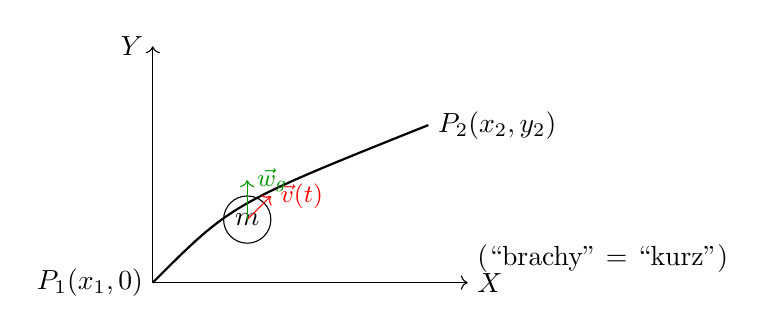
\begin{tikzpicture}
\draw[->] (0,0) -- (4,0) node[right] {$X$} node[above right] {(``brachy'' = ``kurz'')};
\draw[->] (0,0) -- (0,3) node[left] {$Y$};
\draw (0,0) node[left] {$P_1(x_1,0)$};
\draw (3.5,2) node[right] {$P_2(x_2,y_2)$};
\draw[thick] (0,0) .. controls (1,1) .. (3.5,2);
\draw (1.2,0.8) circle (0.3) node {$m$};
\draw[->,red] (1.2,0.8) -- (1.5,1.1) node[right] {\small $\vec{v}(t)$};
\draw[->,green!60!black] (1.2,0.8) -- (1.2,1.3) node[right] {\small $\vec{w}_g$};
\end{tikzpicture}
\end{center}

\textbf{Problemstellung:} Ein Massenpunkt $m$ mit Anfangsgeschwindigkeit null soll sich reibungsfrei im homogenen Gravitationsfeld von $P_1 = (x_1, 0)$ nach $P_2 = (x_2, y_2)$ bewegen. Gesucht ist die Kurve $y(x)$, auf der die benötigte Zeit $T$ minimal ist.

\textbf{Herleitung des Zeitfunktionals:} Die Bahngeschwindigkeit ist gegeben durch:
\[
\|\vec{v}(t)\| = \frac{ds}{dt} \quad \Rightarrow \quad dt = \frac{ds}{v}
\]
mit Bogenlängenelement:
\[
ds = \sqrt{dx^2 + dy^2} = dx \cdot \sqrt{1 + \left( \frac{dy}{dx} \right)^2}
\]
Daraus folgt:
\[
T = \int_{P_1}^{P_2} \frac{ds}{v} = \int_{x_1}^{x_2} \frac{\sqrt{1 + y'^2}}{v} dx
\]

\textbf{Energieerhaltung:} Aus der Energieerhaltung folgt:
\[
\frac{1}{2}mv^2 = mgy \quad \Rightarrow \quad v = \sqrt{2gy}
\]
Daher ergibt sich das Funktional:
\[
T[y] = \int_{x_1}^{x_2} \frac{\sqrt{1 + (y')^2}}{\sqrt{2gy}}\, dx
= \frac{1}{\sqrt{2g}} \int_{x_1}^{x_2} \frac{\sqrt{1 + (y')^2}}{\sqrt{y}}\, dx
\]

\textbf{Euler-Lagrange-Gleichung:} Definiere:
\[
F(y, y') = \frac{1}{\sqrt{2g}} \cdot \frac{\sqrt{1 + (y')^2}}{\sqrt{y}}
\]
Dann liefert die Euler-Lagrange-Gleichung:
\[
\frac{\partial F}{\partial y} - \frac{d}{dx} \left( \frac{\partial F}{\partial y'} \right) = 0
\]

\textbf{Erhaltungsgröße:} Da $F$ nicht explizit von $x$ abhängt, ist die Hamilton-Funktion
\[
H = \frac{\partial F}{\partial y'} \cdot y' - F
\]
entlang Lösungen der Euler-Lagrange-Gleichung konstant.

\textbf{Lösung — Zykloide:} Die Lösung des Problems ist eine Zykloide mit Parameterdarstellung:
\[
\begin{pmatrix} x - x_0 \\ y \end{pmatrix}
= r_0 \begin{pmatrix} \varphi - \sin\varphi \\ 1 - \cos\varphi \end{pmatrix}
\]
Dies entspricht der Bahnkurve eines Punktes auf dem Rand eines rollenden Rades.

Der Parameter $r_0$ wird so gewählt, dass die Kurve durch den Zielpunkt $P_2 = (x_2, y_2)$ verläuft.
\end{EXA}

\begin{CONC}{CM-K25c-12-05}{Hamiltonsche Prinzip}
Darunter versteht man die folgende Aussage (auch genannt ``Prinzip der stationären Wirkung''):

Die Bewegung eines mechanischen Systems von einem gegebenen Anfangspunkt zur Zeit $t_1$ zu einem gegebenen Endpunkt zur Zeit $t_2$ verläuft so, dass die Wirkung $S$ stationär ist,

\[\delta S = 0, \quad S = \int_{t_1}^{t_2} dt\, L(q(t), \dot{q}(t), t)\]

Dies ist die kompakteste Formulierung der klassischen Mechanik: in $\delta S = 0$ ist dieselbe Physik wie in den Lagrange-gleichungen enthalten. Viele Lehrbücher benutzen daher das Hamiltonsche Prinzip als Ausgangspunkt zum formalen Aufbau der Mechanik. Es gilt sowohl für holonome Z.B. als auch für differenzielle Z.B., solange sich die Kräfte aus generalisierten Potentialen herleiten lassen.
\end{CONC}

\begin{CONC}{CM-K25c-12-06}{Hamiltonsche Prinzip und Holonome Zwangsbedingungen}
Sei
\[
  S[q]=\int_{t_1}^{t_2} L\bigl(q,\dot q,t\bigr)\,\mathrm dt,
  \qquad
  L=L(q,\dot q,t)
\]
mit festen Randwerten
$\,\delta q_j(t_1)=\delta q_j(t_2)=0$.  
Die Variation liefert
\[
  \delta S
  =\sum_{j=1}^{n}\!
     \int_{t_1}^{t_2}
       \Bigl[
         \frac{\partial L}{\partial q_j}
        -\frac{\mathrm d}{\mathrm dt}
          \frac{\partial L}{\partial\dot q_j}
       \Bigr]
       \delta q_j\,\mathrm dt .
\]
Da die $\delta q_j$ unabhängig sind, folgen die
\emph{Euler–Lagrange-Gleichungen}
\[
  \boxed{%
    \frac{\mathrm d}{\mathrm dt}
      \frac{\partial L}{\partial\dot q_j}
    -\frac{\partial L}{\partial q_j}=0,
    \qquad j=1,\dots,n } 
\]
– identisch mit den Lagrangegleichungen 2. Art.
\end{CONC}

\begin{CONC}{CM-K25c-12-07}{Hamiltonsche Prinzip und Differenzielle Zwangsbedingungen}
Liegt eine Pfaffsche Nebenbedingung
\[
  \sum_{i=1}^{M} q_{ji}(q,\dot q,t)\,\delta q_i
  + q_{jt}(q,\dot q,t)\,\delta t =0,
  \qquad j=1,\dots,k,
\]
bzw.\ im autonomen Fall  
$\sum_{i}q_{ji}\,\delta q_i =0$ vor, so sind die $\delta q_i$
\emph{nicht} unabhängig.  
Führe für jede Bedingung einen zeitabhängigen
Multiplikator $\lambda_j(t)$ ein und betrachte
\[
  \delta S
  =\int_{t_1}^{t_2}\!
     \Bigl[
        \sum_{i=1}^{M}
          \Bigl(
            \frac{\partial L}{\partial q_i}
           -\frac{\mathrm d}{\mathrm dt}
             \frac{\partial L}{\partial\dot q_i}
          \Bigr)\delta q_i
        +\sum_{j=1}^{k}\lambda_j
          \sum_{i=1}^{M}q_{ji}\,\delta q_i
     \Bigr]\mathrm dt .
\]
Nun gelten die $\delta q_i$ als formal unabhängig und man erhält
\[
  \boxed{%
    \frac{\mathrm d}{\mathrm dt}
      \frac{\partial L}{\partial\dot q_i}
    -\frac{\partial L}{\partial q_i}
    =\sum_{j=1}^{k}\lambda_j\,q_{ji},
    \qquad i=1,\dots,M=3N } 
\]
sowie die $k$ Zwangsgleichungen.  
Dies sind die \textbf{Lagrangegleichungen 1. Art};  
die Größen
$\displaystyle
  K_i^{\,Z}:=\sum_{j}\lambda_j q_{ji}
$
sind die \emph{generalisierten Zwangskräfte}.
\end{CONC}

\begin{REM}{CM-K25c-12-08}{Anmerkung zum Hamiltonschen Prinzip}
\begin{enumerate}
  \item $\delta S=0$ liefert stationäre Bahnen; häufig,
        aber nicht zwingend, ist $S$ dabei minimal.
  \item Im Hamiltonschen Prinzip werden die Bahnen durch
        $q_j(t_1)$ und $q_j(t_2)$ fixiert, nicht durch
        Anfangswerte $(q_j,\dot q_j)$.
  \item Die Wirkung
        $S=\int L\,\mathrm dt$
        bildet das Fundament der Feynmanschen Pfadintegralformulierung
        in der Quantenmechanik.
\end{enumerate}
\end{REM}

\section{Starre Körper}

\subsection{Kinematik starrer Körper}

\begin{CONC}{CM-K25c-13-01}{Setting für Kinematik starrer Körper}
In Mechanik I (Kapitel 8) haben wir die Rotation eines starren Körpers um eine feste Achse untersucht; in diesem Fall gibt es eine formale Analogie zur linearen Bewegung. Ist der Körper jedoch gar nicht oder nur an einem einzigen Punkt fixiert, so ist die Bewegung viel komplizierter. Im folgenden Kapitel 8 werden wir dieses Problem mit Hilfe des Lagrange-Formalismus untersuchen. Zunächst müssen wir jedoch geeignete generalisierte Koordinaten finden, um die Kinematik eines starren Körpers zu beschreiben. Wir erinnern dazu an den Satz von Chasle (siehe Mechanik I, Kap. 8.1, S.204):

Die allgemeine Bewegung eines starren Körpers lässt sich zerlegen in
\begin{enumerate}
\item Translation eines beliebigen Punktes
\item Rotation um diesen Punkt.
\end{enumerate}
\end{CONC}

\begin{CONC}{CM-K25c-13-02}{Setting für Kinematik starrer Körper: Darstellung des Gesamtdrehimpulses}
Gegeben sei ein starrer Körper mit $N$ Massen $m_i$ ($i = 1,\dots,N$), Gesamtmasse $M = \sum_{i=1}^N m_i$. 

\textbf{Kinetische Energie in CM}: Nach König’s Theorem (vgl. Mech.I, S.165) lässt sich die kinetische Energie des Körpers in einen Translations- und Relativanteil zerlegen:
\[
T = \underbrace{\frac{M}{2} \vec{V}_{CM}^2}_{T_{\text{trans}}} + \underbrace{\frac{1}{2} \sum_{i=1}^N m_i \dot{\vec{r}}_i^2}_{T_{\text{rel}}}, \quad \vec{V}_{CM} = \dot{\vec{R}}_{CM}
\]
wobei $\vec{R}_{CM}$ der Schwerpunktvektor im Inertialsystem ist und $\vec{r}_i'$ die Position von Masse $m_i$ im Schwerpunktsystem bezeichnet.

\textbf{Gesamtdrehimpuls in CM}: Der Gesamtdrehimpuls bezüglich eines Ursprungs im Inertialsystem ist ebenfalls in Schwerpunkt- und Relativanteil zerlegbar (Mech.I, S.178):
\[
\vec{L} = \vec{R}_{CM} \times M \dot{\vec{R}}_{CM} + \sum_{i=1}^N \vec{r}_i' \times m_i \dot{\vec{r}}_i'
\]
\textbf{Ursprung im CM}: Im Fall eines fixierten Körpers ist es sinnvoll, den Ursprung in den Fixpunkt zu legen; für einen freibeweglichen Körper liegt der Ursprung meist im Schwerpunkt. In beiden Fällen bleibt nur der Relativanteil übrig:
\[
T = T_{\text{rot}} = \sum_{i=1}^N \frac{m_i}{2} \dot{\vec{r}}_i^2, \qquad
\vec{L} = \sum_{i=1}^N \vec{r}_i \times m_i \dot{\vec{r}}_i
\]
Dabei bezeichnet $\vec{r}_i$ nun die Position relativ zum gewählten Ursprung. 

\textbf{Rotation von starrem Körper und Trägheitstensoren im Inertialsystem}: Für einen starren Körper rotiert $\vec{r}_i$ um diesen Ursprung, also gilt
\[
\dot{\vec{r}}_i = \vec{\omega}(t) \times \vec{r}_i(t)
\]
mit $\vec{\omega}(t)$ als Winkelgeschwindigkeitsvektor (Mech. I, S.206). Wir wenden nun die BAC–CAB-Regel an:
\[
\begin{aligned}
\vec{L} &= \sum_{i=1}^N m_i \vec{r}_i \times (\vec{\omega} \times \vec{r}_i)
= \sum_{i=1}^N m_i \left( \vec{\omega} r_i^2 - \vec{r}_i (\vec{r}_i \cdot \vec{\omega}) \right) \\
T_{\text{rot}} &= \sum_{i=1}^N \frac{m_i}{2} (\vec{\omega} \times \vec{r}_i)^2
= \frac{1}{2} \sum_{i=1}^N m_i \left( \vec{\omega}^2 r_i^2 - (\vec{\omega} \cdot \vec{r}_i)^2 \right)
\end{aligned}
\]
Ein Vergleich ergibt:
\[
\boxed{T_{\text{rot}} = \frac{1}{2} \vec{\omega} \cdot \vec{L}}
\]
Für die Darstellung in der Basis $\{ \vec{e}_1, \vec{e}_2, \vec{e}_3 \}$ definieren wir:
\[
L_\alpha = \vec{e}_\alpha \cdot \vec{L}, \quad r_{i,\alpha} = \vec{e}_\alpha \cdot \vec{r}_i, \quad \omega_\alpha = \vec{e}_\alpha \cdot \vec{\omega}, \quad \alpha = 1,2,3
\]
Im Inertialsystem werden die Vektoren $\vec{L}$, $\vec{r}_i$ und $\vec{\omega}$ dann durch die folgenden Spaltenvektoren dargestellt:
\[
\underset{\sim}{\vec{L}} =
\begin{pmatrix}
L_1 \\
L_2 \\
L_3
\end{pmatrix}
=
\begin{pmatrix}
\vec{e}_1 \cdot \vec{L} \\
\vec{e}_2 \cdot \vec{L} \\
\vec{e}_3 \cdot \vec{L}
\end{pmatrix}, \qquad
\underset{\sim}{\vec{r}_i} =
\begin{pmatrix}
r_{i,1} \\
r_{i,2} \\
r_{i,3}
\end{pmatrix}, \qquad
\underset{\sim}{\vec{\omega}} =
\begin{pmatrix}
\omega_1 \\
\omega_2 \\
\omega_3
\end{pmatrix}
\]
Dann ist
\[
\begin{aligned}
L_\alpha &= \sum_{i=1}^N m_i \left( \omega_\alpha r_i^2 - r_{i,\alpha} \sum_{\beta=1}^3 r_{i,\beta} \omega_\beta \right) \\
&= \sum_{\beta=1}^3 \left[ \sum_{i=1}^N m_i \left( r_i^2 \delta_{\alpha\beta} - r_{i,\alpha} r_{i,\beta} \right) \right] \omega_\beta
= \sum_{\beta=1}^3 I_{\alpha\beta} \omega_\beta
\end{aligned}
\]
wobei Trägheitstensor im Inertialsystem in ausgewählten Basis $\vec{e}_1, \vec{e}_2, \vec{e}_3$ definiert als durch
$$
\begin{aligned}
I_{\alpha\beta} = \sum_{i=1}^N m_i \left(\delta_{\alpha\beta} r_i^2 - r_{i\alpha} r_{i\beta}\right)
\end{aligned}
$$
Die entsprechende 3$\times$3-Matrix:
$$
\begin{aligned}
I = \begin{pmatrix}
I_{11} & I_{12} & I_{13} \\
I_{21} & I_{22} & I_{23} \\
I_{31} & I_{32} & I_{33}
\end{pmatrix}
\end{aligned}
$$
nennt man Darstellung des Trägheitstensors in der Basis $\vec{e}_1,\vec{e}_2,\vec{e}_3$.

(Genau wie Vektoren sind Tensoren durch ihr Transformations-Verhalten bei Drehungen definiert und sind als absolute Objekte unabhängig von einer konkreten Basis. Man unterscheidet daher zwischen absoluten Tensoren und ihren Basis-Darstellungen).

In Matrix-Schreibweise können wir den Zusammenhang $L_\alpha = \sum_\beta I_{\alpha\beta}w_\beta$ auch so schreiben:
$$
\begin{aligned}
\vec{\underset{\sim}{L}} = I \vec{\underset{\sim}{w}}, \quad I = \sum_{i=1}^N m_i \begin{bmatrix}
1 & 0 & 0 \\
0 & 1 & 0 \\
0 & 0 & 1
\end{bmatrix} \vec{\underset{\sim}{r}}_i \vec{\underset{\sim}{r}}_i^T - \vec{\underset{\sim}{r}}_i \vec{\underset{\sim}{r}}_i^T
\end{aligned}
$$
Analog ergibt sich für die kinetische Energie der Rotation:
$$
\begin{aligned}
T_{rot} = \frac{1}{2} \vec{\underset{\sim}{w}}^T \vec{\underset{\sim}{L}} = \frac{1}{2} \vec{\underset{\sim}{w}}^T I \vec{\underset{\sim}{w}}
\end{aligned}
$$



\textbf{Anmerkung:} Bei kontinuierlicher Massenverteilung mit Dichte $\rho(\vec{r})$:

$$
\begin{aligned}
I_{\alpha\beta} = \int d^3r \rho(\vec{r}) \left[\delta_{\alpha\beta} \vec{r}^2 - (\vec{e}_\alpha \cdot \vec{r})(\vec{e}_\beta \cdot \vec{r})\right]
\end{aligned}
$$
\end{CONC}

\begin{CONC}{CM-K25c-13-03}{Transformation in ein körperfestes (rotierendes) Bezugssystem}
Ein starrer Körper lässt sich häufig leichter beschreiben, wenn man in
ein \emph{körperfestes} Bezugssystem übergeht, dessen Achsen die
Rotationsbewegung mitführen.  

\begin{itemize}
  \item Ist der Körper in einem Punkt fixiert, so wählen wir den Ursprung
        sowohl des Inertialsystems als auch des körperfesten Systems in
        diesem Fixpunkt.

  \item Ist der Körper frei beweglich, so legen wir den Ursprung des
        körperfesten Systems in den Schwerpunkt.
\end{itemize}

\vspace{0.5em}

%--------------------------------------------------------------------
\textbf{Rotationsmatrix}

Die zeitabhängige Rotationsmatrix $R(t)\in\mathrm{SO}(3)$ verbindet die
Basen der beiden Bezugssysteme
\[
  \vec e'_\alpha(t)=\sum_{\beta=1}^{3}R_{\alpha\beta}(t)\,\vec e_\beta,
  \qquad
  R_{\alpha\beta}(t)=\vec e'_\alpha(t)\!\cdot\!\vec e_\beta,
  \qquad
  R^{-1}=R^{\mathrm T}.
\]

%--------------------------------------------------------------------
\textbf{Transformation von Vektoren}

\[
  \underline r' = R\,\underline r,
  \qquad
  \underline\omega' = R\,\underline\omega,
  \qquad
  \underline L' = R\,\underline L.
\]

%--------------------------------------------------------------------
\textbf{Trägheitstensor}

Für den Trägheitstensor gilt
\[
  \underline L = I\,\underline\omega
  \;\;\Longrightarrow\;\;
  \underline L' = RIR^{-1}\,\underline\omega'.
\]
Damit definiert man
\[
  I' = R I R^{-1},
\]
und es folgt
\[
  \underline L' = I'\,\underline\omega', 
  \qquad
  T_{\text{rot}} = \tfrac12\,\underline\omega'^{\!\mathrm T}
                   I'\,\underline\omega'.
\]

\textbf{Komponentenform}

\[
  I'_{\alpha\beta}
  =\sum_{\gamma,\delta=1}^{3}
     R_{\alpha\gamma}\,I_{\gamma\delta}\,R_{\beta\delta}.
\]
Da die Schwerpunktskoordinaten $r'_{i,\alpha}
=\vec e'_\alpha\!\cdot\!\vec r_i$ im körperfesten System zeitlich
konstant sind, ist auch $I'$ zeitunabhängig.

\vspace{0.5em}

\noindent
\textbf{Fazit:}  
Der Trägheitstensor transformiert bei einem Wechsel in ein rotierendes
Koordinatensystem nach
\(
  I'\!=\!RIR^{-1},
\)
wodurch er die definierende Eigenschaft eines (Koordinaten-)Tensors
erfüllt.
\end{CONC}

\begin{CONC}{CM-K25c-13-04}{Hauptträgheitsachsen eines starren Körpers}
Wähle das körperfeste Koordinatensystem so, dass der Trägheits­tensor
\[
  I' \;=\; R I R^{\mathrm T}
  \;=\;
  \begin{pmatrix}
    I_1' & 0 & 0 \\
    0 & I_2' & 0 \\
    0 & 0 & I_3'
  \end{pmatrix}
\]
diagonal ist.  
Die Basisvektoren $\vec e_1',\vec e_2',\vec e_3'$ heißen
\emph{Hauptträgheitsachsen},
die Diagonalelemente $I_\alpha'$ die
\emph{Hauptträgheitsmomente}.
Dann gilt
\[
  L_\alpha' = I_\alpha'\,\omega_\alpha',
  \qquad
  T_{\text{rot}}=\tfrac12
    \bigl(I_1'\omega_1'^{2}+I_2'\omega_2'^{2}+I_3'\omega_3'^{2}\bigr).
\]

\textbf{Typische Körperklassen}

\begin{tabular}{@{}ll@{}}
unsymmetrischer Kreisel & $I_1'\neq I_2'\neq I_3'$ \\[2pt]
symmetrischer Kreisel  & $I_1'=I_2'\neq I_3'$ \\[2pt]
Kugelkreisel           & $I_1'=I_2'=I_3'$ \\[2pt]
Rotator (Stab)         & $I_1'=I_2',\;I_3'=0$
\end{tabular}



\textbf{Bestimmung der Hauptachsen}

Suche $R$ so, dass $RIR^{-1}$ diagonal wird.
In Komponentenform
\[
  I R^{-1} = R^{-1}
  \begin{pmatrix}
    I_1' & 0 & 0 \\ 0 & I_2' & 0 \\ 0 & 0 & I_3'
  \end{pmatrix},
\]
was äquivalent zur Eigenwertaufgabe
\[
  I\,\vec e_\beta' = I_\beta'\,\vec e_\beta',
  \qquad
  \vec e_\beta' =
  \begin{pmatrix}
    \vec e_1\!\cdot\!\vec e_\beta'\\
    \vec e_2\!\cdot\!\vec e_\beta'\\
    \vec e_3\!\cdot\!\vec e_\beta'
  \end{pmatrix}.
\]
Die $\vec e_\beta'$ sind Eigen­vektoren, $I_\beta'$ die
Eigen­werte des symmetrischen Tensors $I$.
\end{CONC}

\begin{CONC}{CM-K25c-13-05}{Anmerkungen zur Hauptträgheitsachsen eines starren Körpers}
\begin{enumerate}
  \item Alle Eigenwerte $I_\alpha'$ sind reell.
  \item Die Eigenvektoren können orthonormal gewählt werden
        ($R\in\mathrm{SO}(3)$).
  \item Im Hauptachsensystem sind Trägheits­tensor, Winkelgeschwindigkeit
        und Drehimpuls diagonal verknüpft:
        $\vec L' = I' \vec\omega'$.
        $\vec L$ und $\vec\omega$ sind also parallel
        \emph{genau dann},
        wenn die Rotation um eine Hauptachse erfolgt.
  \item Rotiert der Körper um eine beliebige feste Achse
        (Einheitsvektor $\vec n$ im Inertial­system),
        so lautet das zugehörige Trägheitsmoment
        \[
          I_{\vec n} \;=\;
          \vec n^{\mathrm T} I\,\vec n .
        \]
\end{enumerate}
\end{CONC}

\begin{CONC}{CM-K25c-13-06}{Eulersche Winkel}
Diese bilden einen Satz von unabhängigen generalisierten Koordinaten, die die Lage des starren Körpers relativ zum Ursprung des Inertialsystems (Schwerpunkt bzw. der fixierte Punkt des starren Körpers) eindeutig festlegen. Wegen

\[
\vec{e}_i'(t) = \sum_{j=1}^3 R_{ij}(t) \vec{e}_j \quad \text{(siehe S. 30, mit }\alpha,\beta,\gamma\text{)}
\]

\noindent
müssen wir dazu die Drehmatrix $R_{ij}(t)$ geeignet parametrisieren. Da hier keine Verwechslung mit dem Teilchenindex i auftreten kann, nennen wir den Komponentenindex wieder $\alpha \to i$, $\beta \to j$.

Die Eulerschen Winkel stellen eine mögliche Parametrisierung dar: es sind Drehwinkel in 3 verschiedenen Koordinatensystemen, welche durch die Eulerschen Winkel selbst definiert sind.

Wir zerlegen dazu die durch $R(t)$ beschriebene Drehung in 3 Schritte:

\begin{center}
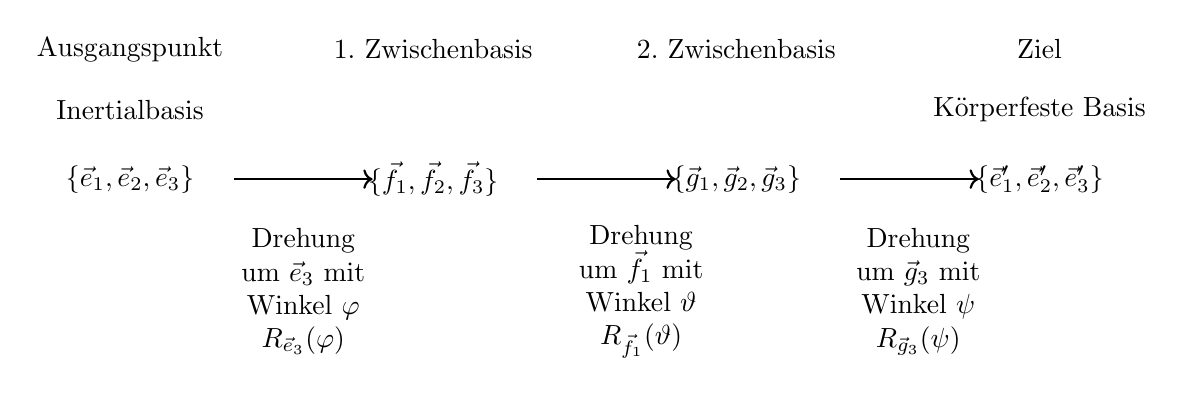
\begin{tikzpicture}[every node/.style={font=\normalsize}, scale=1.1]
% Tabellenüberschriften
\node at (0,4) {Ausgangspunkt};
\node at (3.5,4) {1.~Zwischenbasis};
\node at (7,4) {2.~Zwischenbasis};
\node at (10.5,4) {Ziel};

% Basenbezeichnungen
\node at (0,3.3) {Inertialbasis};
\node at (10.5,3.3) {Körperfeste Basis};

% Basisvektoren
\node at (0,2.5) {$\{\vec{e}_1, \vec{e}_2, \vec{e}_3\}$};
\node at (3.5,2.5) {$\{\vec{f}_1, \vec{f}_2, \vec{f}_3\}$};
\node at (7,2.5) {$\{\vec{g}_1, \vec{g}_2, \vec{g}_3\}$};
\node at (10.5,2.5) {$\{\vec{e}_1', \vec{e}_2', \vec{e}_3'\}$};

% Pfeile zwischen Basen
\draw[->, thick] (1.2,2.5) -- (2.8,2.5);
\draw[->, thick] (4.7,2.5) -- (6.3,2.5);
\draw[->, thick] (8.2,2.5) -- (9.8,2.5);

% Beschreibung der Rotationen
\node[align=center] at (2,1.2) {Drehung\\ um $\vec{e}_3$ mit\\ Winkel $\varphi$\\ $R_{\vec{e}_3}(\varphi)$};
\node[align=center] at (5.9,1.2) {Drehung\\ um $\vec{f}_1$ mit\\ Winkel $\vartheta$\\ $R_{\vec{f}_1}(\vartheta)$};
\node[align=center] at (9.1,1.2) {Drehung\\ um $\vec{g}_3$ mit\\ Winkel $\psi$\\ $R_{\vec{g}_3}(\psi)$};

\end{tikzpicture}
\end{center}
Für die Drehmatrizen ergeben sich die folgenden expliziten Darstellungen:
\noindent

1. Drehung:
\[\vec{f}_i = \sum_{j=1}^3 (R_{\vec{e}_3}(\varphi))_{ij}\vec{e}_j\]

\[R_{\vec{e}_3}(\varphi) = \begin{pmatrix}
\cos\varphi & \sin\varphi & 0 \\
-\sin\varphi & \cos\varphi & 0 \\
0 & 0 & 1
\end{pmatrix}\]

\noindent
2. Drehung:
\[\vec{g}_i = \sum_{j=1}^3 (R_{\vec{f}_1}(\vartheta))_{ij}\vec{f}_j\]

\[R_{\vec{f}_1}(\vartheta) = \begin{pmatrix}
1 & 0 & 0 \\
0 & \cos\vartheta & \sin\vartheta \\
0 & -\sin\vartheta & \cos\vartheta
\end{pmatrix}\]

\noindent
3. Drehung:
\[\vec{e}_i' = \sum_{j=1}^3 (R_{\vec{g}_3}(\psi))_{ij}\vec{g}_j\]

\[R_{\vec{g}_3}(\psi) = \begin{pmatrix}
\cos\psi & \sin\psi & 0 \\
-\sin\psi & \cos\psi & 0 \\
0 & 0 & 1
\end{pmatrix}\]
\end{CONC}

\begin{DEF}{CM-K25c-13-07}{Eulersche Winkel (2)}
\begin{itemize}
  \item \emph{Präzessionswinkel} $\varphi$  
        – Rotation des körperfesten $z'$-Vektors um die Inertial-$z$-Achse.
  \item \emph{Nutationswinkel} $\vartheta$  
        – Neigung des $z'$-Vektors relativ zur Inertial-$z$-Achse.
  \item \emph{Eigenrotationswinkel} $\psi$  
        – Rotation des Körpers um seine eigene $z'$-Achse.
\end{itemize}

Die Gesamtrotation ist das Produkt dreier Basisrotationen

\[
  \boxed{%
    R(\varphi,\vartheta,\psi)
    =R_{\,\vec e_3}(\varphi)\,
     R_{\,\vec f_1}(\vartheta)\,
     R_{\,\vec g_3}(\psi)
  }
\]
wobei $\vec f_1=R_{\,\vec e_3}(\varphi)\vec e_1$ und  
$\vec g_3=R_{\,\vec f_1}(\vartheta)R_{\,\vec e_3}(\varphi)\vec e_3$ die
jeweils „gedrehten“ Achsen sind.  
Für jeden Körpervektor gilt
\[
  \underline r' = R\,\underline r, 
  \qquad
  I'      = R I R^{\mathrm T}.
\]
\end{DEF}

\begin{CONC}{CM-K25c-13-08}{Winkelgeschwindigkeit in körperfester Darstellung}
Mit $\Omega'=\dot R R^{\mathrm T}$ und
$\bigl(\Omega'_{ij}\bigr)=\sum_k\varepsilon_{ijk}\omega_k'$ erhält man

\[
  \boxed{%
    \underline{\omega}'(\varphi,\vartheta,\psi)
    =
    \begin{pmatrix}
      \sin\psi\,\sin\vartheta\,\dot\varphi
      +\cos\psi\,\dot\vartheta \\[4pt]
      \cos\psi\,\sin\vartheta\,\dot\varphi
      -\sin\psi\,\dot\vartheta \\[4pt]
      \cos\vartheta\,\dot\varphi+\dot\psi
    \end{pmatrix}}
\]
\end{CONC}

\begin{CONC}{CM-K25c-13-09}{Rotationsenergie im Hauptachsensystem}
Im körperfesten Hauptachsensystem ($I'=\operatorname{diag}(I_1',I_2',I_3')$)

\[
  T_{\text{rot}}
  =\frac{1}{2}
    \bigl(I_1'\omega_1'^{2}+I_2'\omega_2'^{2}+I_3'\omega_3'^{2}\bigr),
  \qquad
  \underline L'\;=\;I'\underline\omega'.
\]
\end{CONC}

\begin{CONC}{CM-K25c-13-10}{Hauptträgheitsachsen und Eigenwertproblem}
Die Eigenwertaufgabe
\[
  I\,\vec e_\beta' = I_\beta'\,\vec e_\beta',
  \qquad \beta=1,2,3
\]
liefert die orthonormalen Hauptachsen $\vec e_\beta'$ und die
Hauptträgheitsmomente $I_\beta'$.  
Besondere Körper:

\begin{tabular}{@{}ll@{}}
unsymmetrischer Kreisel & $I_1'\neq I_2'\neq I_3'$ \\
symmetrischer Kreisel   & $I_1'=I_2'\neq I_3'$ \\
Kugelkreisel            & $I_1'=I_2'=I_3'$ \\
Rotator (Stab)          & $I_1'=I_2',\ I_3'=0$
\end{tabular}
\end{CONC}

\begin{CONC}{CM-K25c-13-11}{Trägheitsmoment um beliebige Achse}
Für eine feste Drehachse mit Einheitsvektor $\vec n$ gilt
\[
  I_{\vec n}= \vec n^{\mathrm T} I \vec n
  \quad\Longrightarrow\quad
  T_{\text{rot}}=\tfrac12 I_{\vec n}\,\omega^{2}.
\]
\end{CONC}

\subsection{Dynamik starrer Körper}

\begin{CONC}{CM-K25c-14-01}{Eulergleichungen für Winkelgeschwindigkeit}
Ausgangspunkt ist der Drehimpulssatz im Inertialsystem
\[
\frac{\mathrm d}{\mathrm dt}\,\vec L(t)=\vec N(t), 
\qquad 
L_i=\vec e_i\!\cdot\!\vec L,\;
N_i=\vec e_i\!\cdot\!\vec N .
\]

Für ein körperfestes, mitrotierendes System (Basis $\vec e'_\alpha$) gilt mit der Rotationsmatrix $R(t)$
\[
\vec L' = R\,\vec L,
\quad
\vec N' = R\,\vec N,
\quad
\Omega' = \dot R\,R^{\mathrm T},
\qquad 
\Omega'_{ij}=\sum_k\varepsilon_{ijk}\,\omega_k'.
\]

Die Zeitableitung transformiert kovariant
\[
\frac{\mathrm d}{\mathrm dt}\,\vec L' + \Omega'\!\times\!\vec L' = \vec N' ,
\]
denn 
\(
\frac{\mathrm d}{\mathrm dt}\vec L' = \Omega'\vec L' + \vec N'.
\)

Im Hauptachsensystem ist $\vec L' = I'\,\vec\omega'$ mit $I'=\mathrm{diag}(I_1',I_2',I_3')$.  Die Komponentenrelation liefert die \emph{Eulerschen Gleichungen}
\[
\boxed{
\begin{aligned}
I_1'\,\dot\omega_1' - \omega_2'\omega_3'(I_2'-I_3') &= N_1',\\
I_2'\,\dot\omega_2' - \omega_3'\omega_1'(I_3'-I_1') &= N_2',\\
I_3'\,\dot\omega_3' - \omega_1'\omega_2'(I_1'-I_2') &= N_3'.
\end{aligned}}
\]

Hierbei bezeichnen $I_\alpha'$ die Hauptträgheitsmomente, $\omega_\alpha'$ die körperfesten Komponenten der Winkelgeschwindigkeit und $N_\alpha'$ die körperfesten Komponenten des äußeren Drehmoments.
\end{CONC}

\begin{REM}{CM-K25c-14-02}{Anmerkungen zur Euler Gleichungen}
\begin{enumerate}
  \item \textbf{Kräfteloser Kreisel}\,: Für $\vec N = \vec 0$ (also $\vec N'=\vec 0$) bilden die Euler‐Gleichungen ein in sich geschlossenes, nicht-lineares Differentialgleichungssystem für die Winkelgeschwindigkeiten $\omega_i'(t)$.

  \item \textbf{Winkellage}\,: Aus den $\omega_i'(t)$ (bzw.\ $\Omega'=\dot R R^{\mathrm T}$) alleine lässt sich die aktuelle Orientierung des Körpers nicht rekonstruieren; dazu ist die Rotationsmatrix $R(t)$ erforderlich, z.\,B.\ parametrisiert durch die Eulerwinkel $\varphi,\vartheta,\psi$.

  \item \textbf{Starrer Körper im homogenen Gravitationsfeld}\,:  
        Bei $\vec N'\neq\vec 0$ genügen die Euler‐Gleichungen nicht; zusätzlich werden Gleichungen für das äußere Drehmoment benötigt.  
        Für einen um einen Fixpunkt gelagerten Körper im homogenen Feld (Schwerpunktlage $\vec R_{CM}$, Gewichtskraft $\vec F$)
        \[
          \vec N = \vec R_{CM}\times\vec F,
          \qquad
          \vec N' = \vec R'_{CM}\times\vec F',
          \qquad
          \frac{\mathrm d\vec F'}{\mathrm dt}
          = -\,\vec\omega'\times\vec F'.
        \]
\end{enumerate}
\end{REM}

\begin{CONC}{CM-K25c-14-03}{Vollständiges Euler Gleichungssystem im körperfesten Bezug}
\[
\boxed{
\begin{aligned}
I'\,\dot{\vec\omega}' + \vec\omega' \times (I'\vec\omega') &= \vec R_{CM}' \times \vec F', \\[4pt]
\dot{\vec F}' &= -\,\vec\omega' \times \vec F'.
\end{aligned}}
\]

Im kraftfreien Fall ($\vec F'=\vec 0$) reduzieren sich diese sechs Gleichungen auf die drei Euler‐Gleichungen.
\end{CONC}

\begin{CONC}{CM-K25c-14-04}{Kreisel}
Ein \textbf{Kreisel} ist ein starrer Körper, der sich um einen Fixpunkt (oder seinen Schwerpunkt) frei drehen kann.  
\begin{itemize}
\item \textbf{Freier Kreisel}: auf den Körper wirkt \emph{kein} äußeres Drehmoment $\vec N = \vec 0$.  
      Typische Realisierung: Lagerung im Schwerpunkt oder freier Fall im homogenen Schwerefeld.  
\item \textbf{Symmetrischer Kreisel}: zwei Hauptträgheitsmomente sind gleich  
      \[
        I_1'=I_2'\neq I_3',
      \]
      etwa Zylinder, Kreiskegel, Kreisscheibe.
\end{itemize}
\end{CONC}

\begin{CONC}{CM-K25c-14-05}{Euler‐Gleichungen des freien symmetrischen Kreisels im Hauptachsensystem}
Für den freien symmetrischen Kreisel lauten die Euler‐Gleichungen
\[
\begin{aligned}
I_1'\,\dot\omega_1' - (I_1'-I_3')\,\omega_2'\omega_3' &= 0,\\
I_1'\,\dot\omega_2' - (I_3'-I_1')\,\omega_3'\omega_1' &= 0,\\
\dot\omega_3' &= 0\;\Longrightarrow\; \omega_3'=\text{konst}.
\end{aligned}
\]

\textbf{Lösung}

Setze
\[
\Omega=\frac{I_3'-I_1'}{I_1'}\,\omega_3'.
\]
Damit erhält man das gekoppelte System
\[
\dot\omega_1' + \Omega\,\omega_2' = 0,
\qquad
\dot\omega_2' - \Omega\,\omega_1' = 0.
\]
Durch Differentiation folgt die harmonische Gleichung
\[
\ddot\omega_1' + \Omega^2\omega_1' = 0,
\]
mit der Lösung
\[
\boxed{
\begin{aligned}
\omega_1'(t) &= A\cos(\Omega t+\alpha),\\
\omega_2'(t) &= A\sin(\Omega t+\alpha),\\
\omega_3'(t) &= \text{konst}.
\end{aligned}}
\]
\end{CONC}

\begin{CONC}{CM-K25c-14-06}{Bewegung des Winkelgeschwindigkeitsvektors}
\[
\vec\omega'(t)=
\begin{pmatrix}
A\cos(\Omega t+\alpha)\\
A\sin(\Omega t+\alpha)\\
\omega_3'
\end{pmatrix},
\quad
|\vec\omega'|=\sqrt{A^{2}+{\omega_3'}^{2}}=\text{konst}.
\]

\begin{itemize}
\item Die Spitze von $\vec\omega'$ beschreibt einen Kreis radius $A$ um die feste $z'$–Achse des Körpers mit Kreisfrequenz $\Omega$ (\emph{Kreiselkonus}).  
\item Die Beträge $(\omega_1')^{2}+(\omega_2')^{2}$ und $|\vec\omega'|$ bleiben konstant.
\end{itemize}
\end{CONC}

\begin{CONC}{CM-K25c-14-07}{Drehimpuls und Winkelgeschwindigkeit im körperfesten System}
\[
\vec L' \;=\; I'\vec\omega'
           \;=\;
           \begin{pmatrix}
             I_1' A\cos(\Omega t+\alpha)\\
             I_1' A\sin(\Omega t+\alpha)\\
             I_3'\,\omega_3'
           \end{pmatrix},
\qquad
\vec\omega'
           \;=\;
           \begin{pmatrix}
             A\cos(\Omega t+\alpha)\\
             A\sin(\Omega t+\alpha)\\
             \omega_3'
           \end{pmatrix}.
\]

\textbf{Erhaltungsgrößen}

\[
L_3' = I_3'\omega_3' = \text{konst},
\qquad
L_\perp' = \sqrt{(L_1')^{2}+(L_2')^{2}} = I_1' A = \text{konst},
\qquad
|\vec L'| = L = \text{konst}.
\]
\end{CONC}

\begin{CONC}{CM-K25c-14-08}{Kegelförmige Bewegung im Körperfesten System}
Die Spitzen von $\vec\omega'$ und $\vec L'$ umlaufen mit gleicher Kreisfrequenz
\(
  \Omega = \dfrac{I_3'-I_1'}{I_1'}\,\omega_3'
         = \dfrac{I_3'-I_1'}{I_1'I_3'}\,L_3'
\)
einen Kreiskegel um die feste $z'$-Achse.
Die Öffnungswinkel sind
\[
\tan\vartheta_L=\frac{L_\perp'}{L_3'}, 
\qquad
\tan\vartheta_\omega=\frac{A}{\omega_3'}
                    =\frac{I_3'}{I_1'}\tan\vartheta_L .
\]
\end{CONC}

\begin{CONC}{CM-K25c-14-09}{Darstellung der Winkelgeschwindigkeit im Inertialsystem}
Wählt man die Inertial-$z$ Achse in Richtung des konstanten
Drehimpulses $\vec L$, so zerfällt die Winkelgeschwindigkeit in
\[
\vec\omega = \underbrace{\vec\omega_{\!\text{Pr}}}_{\parallel\,\vec L}
             +\underbrace{\vec\omega_{\!\text{Fig}}}_{\parallel\,\vec e_3'},
\quad
\omega_{\!\text{Pr}}=\frac{L}{I_1'},
\quad
\omega_{\!\text{Fig}}=\omega_3' - \omega_{\!\text{Pr}}\cos\vartheta_L
                    = -\,\Omega .
\]
\end{CONC}

\begin{CONC}{CM-K25c-14-10}{Zusammenfassung freien symmetrischen Kreisel}
\begin{itemize}
\item Die Figurenachse führt eine \emph{kräftefreie Präzession} um
      $\vec L$ mit Frequenz $\omega_{\!\text{Pr}}$.
\item Gleichzeitig rotiert der Körper mit
      Eigenfrequenz $\omega_{\!\text{Fig}}=-\Omega$ um seine
      Figurenachse.
\item Für den freien symmetrischen Kreisel sind damit sowohl
      Präzessions- als auch Spingeschwindigkeit ausschließlich durch die
      Erhaltungsgrößen $L$ und $L_3'$ bestimmt.
\end{itemize}
\end{CONC}

\begin{CONC}{CM-K25c-14-11}{Winkellage des freien symmetrischen Kreisels}
Aus
\[
\vec\omega'
=
\begin{pmatrix}
\sin\vartheta\,\sin\psi+\cos\vartheta\,\dot\varphi\\[2pt]
\sin\vartheta\,\cos\psi-\dot\vartheta\,\sin\psi\\[2pt]
\cos\vartheta\,\dot\varphi+\dot\psi
\end{pmatrix}
=
\begin{pmatrix}
A\cos(\Omega t+\alpha)\\
A\sin(\Omega t+\alpha)\\
\omega_3'
\end{pmatrix},
\qquad
\Omega=\frac{I_3'-I_1'}{I_1'}\,\omega_3',
\]
folgt im gewählt­en Inertialsystem ($\vec e_3\parallel\vec L$):

\begin{enumerate}
\item \(\vartheta(t)=\vartheta_L=\text{konst}\).

\item Erste beiden Komponenten liefern  
      \(\sin\vartheta_L\,\dot\varphi=\pm A\)  
      \(\Longrightarrow\)
      \[
        \dot\varphi=\pm\omega_{\text{Pr}}\!,
        \qquad
        \omega_{\text{Pr}}=\frac{A}{\sin\vartheta_L}
                          =\frac{L}{I_1'},
        \qquad
        \varphi(t)=\pm\omega_{\text{Pr}}\,t+\varphi_0 .
      \]

\item Dritte Komponente gibt  
      \[
        \dot\psi
        =\omega_3'-\cos\vartheta_L\,\dot\varphi
        =\omega_3'\mp\omega_{\text{Pr}}\cos\vartheta_L
        =-\Omega,
        \qquad
        \psi(t)=-\Omega t-\alpha\pm\frac{\pi}{2}.
      \]
\end{enumerate}

Damit ist die vollständige zeitabhängige Orientierungsbeschreibung des freien symmetrischen Kreisels durch die drei Eulerwinkel
\(
  \vartheta(t)=\vartheta_L,\;
  \varphi(t)=\pm\omega_{\text{Pr}}t+\varphi_0,\;
  \psi(t)=-\Omega t-\alpha\pm\frac{\pi}{2}
\)
gegeben.
\end{CONC}

\begin{CONC}{CM-K25c-14-12}{Winkellage des freien symmetrischen Kreisels}
Aus
\[
\vec\omega'
=
\begin{pmatrix}
\sin\vartheta\,\sin\psi+\cos\vartheta\,\dot\varphi\\[2pt]
\sin\vartheta\,\cos\psi-\dot\vartheta\,\sin\psi\\[2pt]
\cos\vartheta\,\dot\varphi+\dot\psi
\end{pmatrix}
=
\begin{pmatrix}
A\cos(\Omega t+\alpha)\\
A\sin(\Omega t+\alpha)\\
\omega_3'
\end{pmatrix},
\qquad
\Omega=\frac{I_3'-I_1'}{I_1'}\,\omega_3',
\]
folgt im gewählt­en Inertialsystem ($\vec e_3\parallel\vec L$):

\begin{enumerate}
\item \(\vartheta(t)=\vartheta_L=\text{konst}\).

\item Erste beiden Komponenten liefern  
      \(\sin\vartheta_L\,\dot\varphi=\pm A\)  
      \(\Longrightarrow\)
      \[
        \dot\varphi=\pm\omega_{\text{Pr}}\!,
        \qquad
        \omega_{\text{Pr}}=\frac{A}{\sin\vartheta_L}
                          =\frac{L}{I_1'},
        \qquad
        \varphi(t)=\pm\omega_{\text{Pr}}\,t+\varphi_0 .
      \]

\item Dritte Komponente gibt  
      \[
        \dot\psi
        =\omega_3'-\cos\vartheta_L\,\dot\varphi
        =\omega_3'\mp\omega_{\text{Pr}}\cos\vartheta_L
        =-\Omega,
        \qquad
        \psi(t)=-\Omega t-\alpha\pm\frac{\pi}{2}.
      \]
\end{enumerate}

Damit ist die vollständige zeitabhängige Orientierungsbeschreibung des freien symmetrischen Kreisels durch die drei Eulerwinkel
\(
  \vartheta(t)=\vartheta_L,\;
  \varphi(t)=\pm\omega_{\text{Pr}}t+\varphi_0,\;
  \psi(t)=-\Omega t-\alpha\pm\frac{\pi}{2}
\)
gegeben.
\end{CONC}

\begin{CONC}{CM-K25c-14-13}{Bewegung des freien symmetrischen Kreisels – Überblick}
Der Bewegungsablauf ist die \emph{Überlagerung zweier stetiger Drehungen}:

\textbf{1) Präzession der Figurenachse}\\
Die feste $z^{\prime}$-Achse (Figurenachse) beschreibt einen Kreiskegel um den \emph{konstanten} Drehimpuls­vektor $\vec L$  
\[
\omega_{\text{Prä}}=\dot{\varphi}= \frac{L}{I_1'},
\qquad
\vartheta=\vartheta_L=\text{konst}.
\]

\textbf{2) Eigenrotation um die Figurenachse}\\
Gleichzeitig rotiert der Körper mit konstanter Winkelgeschwindigkeit  
\[
\omega_{\text{Fig}}=\dot{\psi}
          =-\Omega
          =\Bigl(1-\tfrac{I_3'}{I_1'}\Bigr)\frac{L_3'}{I_3'}
          =\frac{I_1'-I_3'}{I_1'}\,\omega_3'.
\]

\bigskip
\textbf{Beispiel: Erde als nahezu symmetrischer Kreisel}

\[
\frac{I_3'-I_1'}{I_1'}\simeq\frac{1}{300},
\qquad
\omega_3'=\frac{2\pi}{1\;\text{Tag}}
\Longrightarrow
\omega_{\text{Fig}}\approx\frac{2\pi}{300\;\text{Tage}}.
\]

Die beobachtete sogenannte Chandler-Periode liegt bei etwa $427$ Tagen; die Differenz zum starren-Körper-Wert entsteht durch die elastische Deformierbarkeit der Erde.
\end{CONC}

\begin{CONC}{CM-K25c-14-14}{Symmetrische Kreisel im Schwere-Feld}
Wir untersuchen einen \emph{symmetrischen Kreisel} ($I_1'=I_2'\neq I_3'$), dessen Spitze $O$ festgehalten ist, während sich sein Schwerpunkt $C$ im homogenen Schwerefeld befindet. Die Euler­winkel $(\varphi,\vartheta,\psi)$ geben die Lage der Figurenachse $\vec e_3'$ relativ zum Inertialsystem $(\vec e_1,\vec e_2,\vec e_3)$ an.  

\textbf{Lagrange-Funktion}\\
\[
L = \frac{I_1'}{2}\bigl(\dot\vartheta^{\,2}+\dot\varphi^{\,2}\sin^{2}\vartheta\bigr)
    +\frac{I_3'}{2}\bigl(\dot\varphi\cos\vartheta+\dot\psi\bigr)^{2}
    -Mg\ell\cos\vartheta .
\]

\textbf{Erhaltungsgrößen (zyklische Koordinaten)}  
\[
\begin{aligned}
p_\varphi &= I_1'\sin^{2}\vartheta\,\dot\varphi
           +I_3'(\dot\varphi\cos\vartheta+\dot\psi)\cos\vartheta
           =L_3=\text{konst},\\[4pt]
p_\psi    &= I_3'(\dot\varphi\cos\vartheta+\dot\psi)
           =L_3'=\text{konst},\qquad
p_\psi/I_3'=\omega_3'.
\end{aligned}
\]

\textbf{Ausdrücke für $\dot\varphi$ und $\dot\psi$}  
\[
\dot\varphi = \frac{L_3-L_3'\cos\vartheta}{I_1'\sin^{2}\vartheta},
\qquad
\dot\psi    = \frac{L_3'}{I_3'}
             -\dot\varphi\cos\vartheta .
\]

\textbf{Energieerhaltung}\\
\[
E = \frac{I_1'}{2}\dot\vartheta^{\,2}
    +\frac{(L_3-L_3'\cos\vartheta)^{2}}{2I_1'\sin^{2}\vartheta}
    +\frac{L_3'^{2}}{2I_3'}
    +Mg\ell\cos\vartheta .
\tag{3}
\]
\end{CONC}

\begin{CONC}{CM-K25c-14-15}{Interpretation als effektive Ein-Dimensionalität}
Schreibe $E= \tfrac{I_1'}{2}\dot\vartheta^{\,2}+V_{\text{eff}}(\vartheta)$ mit
\[
V_{\text{eff}}(\vartheta)=
  \frac{(L_3-L_3'\cos\vartheta)^{2}}{2I_1'\sin^{2}\vartheta}
  +Mg\ell\cos\vartheta+\frac{L_3'^{2}}{2I_3'} ,
\]
so dass die Bewegung in $\vartheta(t)$ einer eindimensionalen Teilchenbewegung im Potential $V_{\text{eff}}$ entspricht.  
\begin{itemize}
\item Mögliche Nutationswinkel $\vartheta_{\min}\le\vartheta(t)\le\vartheta_{\max}$ ergeben sich aus \(E=V_{\text{eff}}(\vartheta)\).
\item Stetige Präzession ohne Nutation liegt vor, wenn $E=V_{\text{eff}}(\vartheta_L)$ und $\dot\vartheta=0$. Dann bleibt $\vartheta$ konstant, und aus der obigen Gleichung folgt die Gleichgewichtsbedingung des \emph{stationären Kreisels}.
\item Für allgemeine $E$ oszilliert $\vartheta(t)$ zwischen den beiden Wendewinkeln; $\varphi(t)$ und $\psi(t)$ erhält man anschließend durch einmaliges Integrieren der oben angegebenen $\dot\varphi(\vartheta)$, $\dot\psi(\vartheta)$.
\end{itemize}
\end{CONC}

\begin{CONC}{CM-K25c-14-16}{Spezialfall Erde (leicht abgeplatteter Kreisel}
\(
\dfrac{I_3'-I_1'}{I_1'}\simeq \tfrac1{300},\;
\omega_3'=\tfrac{2\pi}{1\text{ Tag}}
\Longrightarrow
\omega_{\text{Fig}}=\dot\psi\approx \tfrac{2\pi}{300\text{ Tage}},
\)
während die beobachtete Chandler-Periode \( \approx 427\text{ Tage} \)
auf die Elastizität der Erde zurückzuführen ist.
\end{CONC}

\begin{CONC}{CM-K25c-14-17}{Reduzierte Bewegungsgleichung durch Erhaltungsgrößen}
Die drei Erhaltungsgrößen $L_3$, $L_3'$, $E$ erlauben es, das System auf eine Differentialgleichung erster Ordnung für den Nutationswinkel zu reduzieren.  

\[
E=\frac{I_1'}{2}\dot{\vartheta}^{\,2}
   +\frac{(L_3-L_3'\cos\vartheta)^{2}}{2I_1'\sin^{2}\vartheta}
   +\frac{L_3'^{2}}{2I_3'}+Mg\ell\cos\vartheta .
\]

Substituiere $\mu=\cos\vartheta$:
\[
\dot{\vartheta}^{\,2}
  =\frac{\dot{\mu}^{\,2}}{1-\mu^{2}},\qquad
1-\mu^{2}=\sin^{2}\vartheta .
\]

Damit erhält man
\[
\dot{\mu}^{\,2}
 =\Bigl[\frac{2I_3'E-L_3'^{2}}{I_1'I_3'}-\frac{2Mg\ell}{I_1'}\mu\Bigr](1-\mu^{2})
   -\Bigl(\tfrac{L_3-L_3'\mu}{I_1'}\Bigr)^{2}
 =-2U_{\text{eff}}(\mu),
\]
\[
U_{\text{eff}}(\mu)
  =\tfrac12\Bigl(\tfrac{L_3-L_3'\mu}{I_1'}\Bigr)^{2}
   -\Bigl[\tfrac{I_3'E-L_3'^{2}}{I_1'I_3'}
          -\tfrac{Mg\ell}{I_1'}\mu\Bigr](1-\mu^{2}).
\]

Damit reduziert sich die Bewegungsgleichung auf

\[
t-t_0
  =\pm\!\int_{\mu_0}^{\mu(t)}
       \frac{\mathrm d\mu'}
            {\sqrt{-2U_{\text{eff}}(\mu')}} .
\]

Die Wendewerte $\mu_{\min}$, $\mu_{\max}$ folgen aus $U_{\text{eff}}(\mu)=0$ und bestimmen den Nutationsbereich $\vartheta_{\max}\le\vartheta\le\vartheta_{\min}$.
\end{CONC}

\begin{CONC}{CM-K25c-14-18}{Reduktion auf eine eindimensionale Bewegung}
Setze
\[
U_{\text{eff}}(\vartheta)=
  \frac{(L_3-L_3'\cos\vartheta)^{2}}{2I_1'\sin^{2}\vartheta}
  +Mg\ell\cos\vartheta ,
\qquad
E=\frac{I_1'}{2}\dot{\vartheta}^{2}+U_{\text{eff}}(\vartheta).
\tag{3$'$}
\]
Damit bewegt sich \(\vartheta(t)\) wie ein Punktteilchen der Masse
\(I_1'\) in dem Potential \(U_{\text{eff}}(\vartheta)\).

\textbf{Stationäre (reine) Präzession}

Reine Präzession liegt vor, wenn \(\dot{\vartheta}=0\) und
\(\vartheta\) konstant bleibt.  
Bedingung:
\[
\frac{\mathrm dU_{\text{eff}}}{\mathrm d\vartheta}=0
\;\;\Longrightarrow\;\;
Mg\ell I_1'\sin\vartheta
=\Bigl(L_3-L_3'\cos\vartheta\Bigr)L_3'.
\]
Die zugehörige Präzessionsfrequenz folgt aus
\[
\dot{\varphi}
 =\frac{L_3-L_3'\cos\vartheta}{I_1'\sin^{2}\vartheta},
\qquad
\dot{\psi}
 =\frac{L_3'}{I_3'}-\dot{\varphi}\cos\vartheta .
\]

\textbf{Nutation}

Ist \(E>U_{\text{eff,min}}\), so oszilliert \(\vartheta(t)\) zwischen
den Wendewinkeln \(\vartheta_{\min },\vartheta_{\max }\) —
bestimmt durch \(E=U_{\text{eff}}(\vartheta)\).  
Das Integral
\[
t-t_0
 =\pm\int_{\vartheta_0}^{\vartheta(t)}
     \sqrt{\frac{I_1'}{2}}
     \frac{\mathrm d\vartheta'}
          {\sqrt{E-U_{\text{eff}}(\vartheta')}} 
\]
liefert \(\vartheta(t)\); anschließendes Einsetzen in
\eqref{1},\eqref{2} liefert \(\varphi(t),\psi(t)\).

\textbf{Grenzfälle}

\begin{itemize}
\item \(\ell\to 0\) (Spitze im Schwerpunkt) $\Rightarrow$
      \(U_{\text{eff}}\to\) konst.; man erhält sofort den
      klassischen freien symmetrischen Kreisel.
\item \(L_3'\to 0\) (keine Eigenrotation) $\Rightarrow$
      Aufrichten ist unmöglich, der Kreisel fällt wie ein starrer Stab.
\item Schlafer Kreisel:
      für \(L_3\!\approx\!L_3'\) und große \(\omega_3'\) kann
      \(\vartheta\) sehr klein werden; dann ist
      \(U_{\text{eff}}\) annähernd quadratisch und 
      kleine Nutations­schwingungen haben die Frequenz
      \(\displaystyle
        \omega_{\text{Nut}}
        \simeq\sqrt{\frac{Mg\ell}{I_3'}}\).
\end{itemize}

\textbf{Zusammenfassung}

Durch die drei Erhaltungsgrößen
\(
  L_3,\;L_3',\;E
\)
wird die schwere symmetrische Top-Dynamik auf die eindimensionale
Bewegung in \(U_{\text{eff}}(\vartheta)\) reduziert.
Aus \(\vartheta(t)\) erhält man die Präzessions- und Eigenrotations­
winkel durch einmaliges Integrieren.
\end{CONC}

\begin{REM}{CM-K25c-14-19}{Graphische Veranschaulichung der Bewegung – Figurenachse auf der Einheitskugel}
\begin{itemize}
  \item Lege eine Einheitskugel um den festen Punkt $O$.  
        Die Spitze der Figurenachse $\vec e_3'(t)$ beschreibt auf dieser Kugel eine Raumkurve.
  \item \emph{Nutation}: Änderung des Polarwinkels $\vartheta(t)$ – Auf– und Ab­schwingen der Figurenachse.
  \item \emph{Präzession}: Änderung des Azimutwinkels $\varphi(t)$ – Umlauf der Figurenachse um die raumfeste $z$-Achse.  
        \[
          \dot\varphi
          =\frac{L_3-L_3'\cos\vartheta}{I_1'\sin^{2}\vartheta}.
        \]
\end{itemize}
\end{REM}

\begin{CONC}{CM-K25c-14-20}{Klassifikation der Bahnen (abhängig von den Anfangsdaten)}
Sei $\vartheta_1\le\vartheta\le\vartheta_2$ das von der Energie zulässige Nutationsintervall.  
Die Gleichung $\dot\varphi=0$ hat Lösungen, falls
\[
  \cos\vartheta_0=\frac{L_3}{L_3'}\in[-1,1].
\]

\begin{enumerate}
  \item $\cos\vartheta_0\notin[\cos\vartheta_1,\cos\vartheta_2]$  
        $\Rightarrow\;\dot\varphi$ behält während der gesamten Nutation sein Vorzeichen.  
        Die Raumkurve ist im Allgemeinen \emph{nicht} geschlossen.
  \item $\cos\vartheta_0\in(\cos\vartheta_1,\cos\vartheta_2)$  
        $\Rightarrow\;\dot\varphi$ wechselt im Laufe der Nutation das Vorzeichen.  
        Die Figurenachse pendelt vor und zurück: \emph{rückläufige Präzession}.
  \item Grenzfall $\cos\vartheta_0=\cos\vartheta_1$ (bzw.\ $=\cos\vartheta_2$)  
        \[
          U_{\mathrm{eff}}(\vartheta_1)=0,
          \quad
          E-\frac{L_3'^{2}}{2I_3'}-Mg\ell\cos\vartheta_1=0.
        \] 
        Die Bahn berührt das „Polhöhen-Extrem“ ohne es zu überschreiten.
  \item Grenzfall $\vartheta_1=\vartheta_2$ (reine Präzession)  
        \[
          \vartheta=\text{konst},
          \qquad
          \dot\varphi=\frac{L_3-L_3'\cos\vartheta}{I_1'\sin^{2}\vartheta}=\text{konst}.
        \]
        Die Figurenachse beschreibt einen Kreis: \emph{reguläre (stationäre) Präzession}.
\end{enumerate}
\end{CONC}

\section{Schwingungen}

\subsection{Grundlagen}

\begin{CONC}{CM-K25c-15-01}{Gedämpfte harmonische Schwingungen}
Bewegungsgleichung  
\[
\ddot x + 2\gamma\dot x + \omega_{0}^{2}x = 0,
\qquad
\omega_{0}^{2}=k/m,
\qquad
\gamma=\alpha/2m .
\]

\textbf{Kennzahlen}  
\[
\lambda_{1,2}=-\gamma\pm\sqrt{\gamma^{2}-\omega_{0}^{2}},
\qquad
\omega_{\text{d}}=\sqrt{\omega_{0}^{2}-\gamma^{2}}\quad
(\text{unterkritisch}) .
\]

\textbf{Lösungen}

\begin{enumerate}
  \item \emph{Unterkritische Dämpfung} \(\gamma^{2}<\omega_{0}^{2}\)  
        \[
          x(t)=A\,e^{-\gamma t}\cos\!\bigl(\omega_{\mathrm d}t-\phi\bigr),
          \qquad
          \omega_{\mathrm d}=\sqrt{\omega_{0}^{2}-\gamma^{2}} .
        \]
        Exponentiell abklingende Schwingung mit der gedämpften Kreisfrequenz
        \(\omega_{\mathrm d}\).

  \item \emph{Kritische Dämpfung} \(\gamma^{2}=\omega_{0}^{2}\)  
        \[
          x(t)=\bigl(A_{1}+A_{2}t\bigr)\,e^{-\gamma t}.
        \]
        Schnellstmögliche Rückkehr zur Ruhelage ohne Oszillation.

  \item \emph{Überkritische Dämpfung} \(\gamma^{2}>\omega_{0}^{2}\)  
        \[
          x(t)=A_{1}e^{\lambda_{1}t}+A_{2}e^{\lambda_{2}t},
          \qquad
          \lambda_{1,2}=-\gamma\pm\sqrt{\gamma^{2}-\omega_{0}^{2}}<0 .
        \]
        Monotones Ausschwingen ohne Nullstellenwechsel.
\end{enumerate}


\textbf{Logarithmisches Dekrement \(\delta\)}  
\[
\delta=\ln\frac{x(t)}{x(t+T_{\text{d}})}
      =2\pi\frac{\gamma}{\omega_{\text{d}}},
\qquad
T_{\text{d}}=2\pi/\omega_{\text{d}} .
\]

\textbf{Qualitätsfaktor \(Q\)}  
\[
Q=\frac{\omega_{0}}{2\gamma}
  =\frac{\pi}{\delta}.
\]

\textbf{Energieabnahme}  
\[
E(t)=\tfrac12kA^{2}e^{-2\gamma t},
\qquad
\tau=\frac{1}{\gamma}\quad\text{(Abklingzeit)}.
\]
\end{CONC}

\begin{CONC}{CM-K25c-15-02}{Erzwungene gedämpfte Schwingung}
\[
\ddot x + 2\gamma\dot x + \omega_{0}^{2}x
  = f_{0}\cos\Omega t,
  \qquad
  f_{0}=\frac{F_{0}}{m}.
\]

\textbf{Spezielle stationäre Lösung}  
Ansatz $z(t)=D e^{i(\Omega t-\varphi)}$ liefert  
\[
D(\Omega)=\frac{F_{0}}
               {\sqrt{(\omega_{0}^{2}-\Omega^{2})^{2}+4\gamma^{2}\Omega^{2}}},
\qquad
\varphi(\Omega)=\arctan\!\Bigl(\frac{2\gamma\Omega}
                                      {\omega_{0}^{2}-\Omega^{2}}\Bigr).
\]

\textbf{Allgemeine Lösung}  
\[
x(t)=x_{h}(t)+D(\Omega)\cos\bigl(\Omega t-\varphi(\Omega)\bigr),
\]
mit
\(x_{h}(t)=A_{0}e^{-\gamma t}\cos\bigl(\sqrt{\omega_{0}^{2}-\gamma^{2}}\,t-\psi_{0}\bigr)\).
Für \(t\gg 1/\gamma\) klingt $x_{h}(t)$ ab und es bleibt die \emph{stationäre} Schwingung.

\textbf{Resonanz bei schwacher Dämpfung \(\gamma<\omega_{0}/2\)}

\[
\Omega_{\text{res}}=\sqrt{\omega_{0}^{2}-2\gamma^{2}},
\qquad
D_{\max}=D(\Omega_{\text{res}})
         =\frac{F_{0}}{2\gamma\sqrt{\omega_{0}^{2}-\gamma^{2}}}.
\]

\textbf{Gütefaktor}

\[
Q=\frac{\Omega_{\text{res}}}{2\gamma}
  =\frac{\sqrt{\omega_{0}^{2}-2\gamma^{2}}}{2\gamma}
  \;\stackrel{\gamma\ll\omega_{0}}{\longrightarrow}\;
  \frac{\omega_{0}}{2\gamma}.
\]

$Q$ ist umgekehrt proportional zur Peakbreite
\(\Delta\Omega\) bei $D(\Omega_{\text{res}})/\sqrt{2}$.
\end{CONC}

\begin{CONC}{CM-K25c-15-03}{Resonanz}
Schwach gedämpfte Oszillationen (\(\gamma < \tfrac{\omega_0}{2}\)) zeigen \emph{Resonanz}.  
Die Amplitude 
\[
  D(\Omega)=\frac{F_0}
                 {\sqrt{(\omega_0^{2}-\Omega^{2})^{2}+4\gamma^{2}\Omega^{2}}}
\]
besitzt dann ein Maximum bei
\[
  \boxed{\;\Omega_{\text{res}}
         =\sqrt{\omega_{0}^{2}-2\gamma^{2}}\;}
\]
(etwas kleiner als die Eigenfrequenz  
\(\omega_{\mathrm d}=\sqrt{\omega_{0}^{2}-\gamma^{2}}\)  
der frei gedämpften Schwingung).

Maximale Amplitude
\[
  \boxed{\;
    D_{\max}=D(\Omega_{\text{res}})
            =\frac{F_0}{2\gamma\sqrt{\omega_{0}^{2}-\gamma^{2}}}\;}
\]

\textbf{Gütefaktor} (dimensionsloses Maß für die Resonanzschärfe)
\[
  \boxed{\;
    Q=\frac{\Omega_{\text{res}}}{2\gamma}
      =\frac{\sqrt{\omega_{0}^{2}-2\gamma^{2}}}{2\gamma}\;}
  \;\xrightarrow{\gamma\ll\omega_{0}}\;
  Q\approx\frac{\omega_{0}}{2\gamma}.
\]

Für kleine Dämpfung (\(Q\gg 1\)) liegt die Halbwertsbreite des Amplituden­peaks bei
\[
  \Delta\Omega \approx 2\gamma
  \quad\Longrightarrow\quad
  Q = \frac{\omega_{0}}{\Delta\Omega}.
\]
\end{CONC}

\begin{CONC}{CM-K25c-15-04}{Erzwungene Schwingungen – periodische Kräfte und Fourier}
Gesucht ist die allgemeine Lösung der inhomogenen linearen DGL
\[
  \ddot{x}+2\gamma\dot{x}+\omega_{0}^{2}x=f(t),
  \qquad
  f(t+T)=f(t),
  \qquad
  F(t)=m\,f(t).
\]

%--------------------------------------------------------------
\textbf{Fourier‐Zerlegung der Anregung}

Für eine stückweise stetige, stückweise stetig differenzierbare
periodische Funktion gilt der Fundamentalsatz der Fourier‐Reihen:
\[
  f(t)=\frac{a_{0}}{2}
       +\sum_{n=1}^{\infty}\!
          \bigl[a_{n}\cos(\Omega_{n}t)+b_{n}\sin(\Omega_{n}t)\bigr],
  \quad
  \Omega_{n}=\frac{2\pi n}{T},
\]
\[
  a_{n}=\frac{2}{T}\!\!\int_{-T/2}^{T/2}\!f(t)\cos(\Omega_{n}t)\,\mathrm dt,
  \quad
  b_{n}=\frac{2}{T}\!\!\int_{-T/2}^{T/2}\!f(t)\sin(\Omega_{n}t)\,\mathrm dt.
\]

Komplexe Schreibweise (kompakter in Rechnungen)
\[
  f(t)=\sum_{n=-\infty}^{\infty}f_{n}\,e^{i\Omega_{n}t},
  \qquad
  f_{n}=\frac{1}{T}\!\!\int_{-T/2}^{T/2}\!f(t)e^{-i\Omega_{n}t}\,\mathrm dt .
\]

%--------------------------------------------------------------
\textbf{Stationäre (periodische) Lösung}

Die stationäre spezielle Lösung wird ebenfalls periodisch sein, also
\[
  x_{s}(t)=\sum_{n=-\infty}^{\infty}x_{n}\,e^{i\Omega_{n}t}.
\]

Einsetzen in die DGL ergibt
\[
  \sum_{n=-\infty}^{\infty}
    e^{i\Omega_{n}t}\!
    \bigl[-\Omega_{n}^{2}+2i\gamma\Omega_{n}+\omega_{0}^{2}\bigr]x_{n}
  =\sum_{n=-\infty}^{\infty}f_{n}e^{i\Omega_{n}t}.
\]

Nach Orthogonalisierung (\(\tfrac1T\int e^{-i(\Omega_{m}-\Omega_{n})t}\,\mathrm dt=\delta_{mn}\))
erhält man für jedes $n$
\[
  x_{n}=\frac{f_{n}}
              {\omega_{0}^{2}-\Omega_{n}^{2}+2i\gamma\Omega_{n}} .
\]

Damit lautet die stationäre Lösung
\[
  x_{s}(t)=
    \sum_{n=-\infty}^{\infty}
      \frac{f_{n}\,e^{i\Omega_{n}t}}
           {\omega_{0}^{2}-\Omega_{n}^{2}+2i\gamma\Omega_{n}} .
\]

%--------------------------------------------------------------
\textbf{Allgemeine Lösung}

Die vollständige Lösung setzt sich aus der stationären Lösung und der
allgemeinen Lösung \(x_{h}(t)\) der homogenen Gleichung zusammen:
\[
  x(t)=x_{h}(t)+x_{s}(t),
  \qquad
  x_{h}(t)=
  \begin{cases}
    A\,e^{-\gamma t}\cos\bigl(\omega_{\mathrm d}t-\phi\bigr),
    &\gamma^{2}<\omega_{0}^{2},\\[6pt]
    (A_{1}+A_{2}t)e^{-\gamma t},
    &\gamma^{2}=\omega_{0}^{2},\\[6pt]
    A_{1}e^{\lambda_{1}t}+A_{2}e^{\lambda_{2}t},
    &\gamma^{2}>\omega_{0}^{2},
  \end{cases}
\]
wobei
\(\omega_{\mathrm d}=\sqrt{\omega_{0}^{2}-\gamma^{2}}\) und
\(\lambda_{1,2}=-\gamma\pm\sqrt{\gamma^{2}-\omega_{0}^{2}}\).

\emph{Einschwingverhalten:}
Für \(t\gg 1/\gamma\) klingt \(x_{h}(t)\) exponentiell ab und die
Bewegung geht in die reine stationäre, mit \(f(t)\) phasenverschobene
Schwingung über:
\[
  x(t)\;\xrightarrow{t\gg1/\gamma}\;x_{s}(t).
\]
Hierbei liefert
\(\varphi_{n}=\arg\bigl[\omega_{0}^{2}-\Omega_{n}^{2}+2i\gamma\Omega_{n}\bigr]\)
die Phasendifferenz zwischen der $n$-ten Harmonischen der Kraft und der
Antwort.
\end{CONC}

\begin{CONC}{CM-K25c-15-05}{Erzwungene Schwingungen – beliebige Antriebskraft und Green}
Betrachte den gedämpften Oszillator mit beliebigem Kraft­term
\[
  \ddot x+2\gamma\dot x+\omega_{0}^{2}x=f(t),
  \qquad 
  F(t)=m\,f(t).
\]

\textbf{1.\ Fourier­transformierte der Anregung}

Für eine absolut integrierbare Kraft $f(t)$ sei  
\[
  \tilde f(\omega)=\int_{-\infty}^{\infty}\!f(t)\,e^{-i\omega t}\,\mathrm dt,
  \qquad
  f(t)=\int_{-\infty}^{\infty}
          \frac{\mathrm d\omega}{2\pi}\,
          \tilde f(\omega)\,e^{i\omega t}.
\]
Diese Darstellung erhält man aus der komplexen Fourier­reihe im Limes
\(T\to\infty\).

\textbf{2.\ Ansatz für die spezielle Lösung}

Die stationäre Antwort schreibe ebenfalls als Fourier­integral
\[
  x_s(t)=\int_{-\infty}^{\infty}
           \frac{\mathrm d\omega}{2\pi}\,
           \tilde x(\omega)\,e^{i\omega t}.
\]

Einsetzen in die DGL liefert für jedes \(\omega\)
\[
  (-\omega^{2}+2i\gamma\omega+\omega_{0}^{2})\tilde x(\omega)=\tilde f(\omega)
  \quad\Longrightarrow\quad
  \boxed{\;
    \tilde x(\omega)=
      \frac{\tilde f(\omega)}
           {\omega_{0}^{2}-\omega^{2}+2i\gamma\omega}}\;.
\]

\textbf{3.\ Retardierte Green‐Funktion}

Definiere
\[
  G(\tau)=
  \int_{-\infty}^{\infty}
     \frac{\mathrm d\omega}{2\pi}\,
     \frac{e^{i\omega\tau}}
          {\omega_{0}^{2}-\omega^{2}+2i\gamma\omega}.
\]
Für \(\omega_{0}^{2}>\gamma^{2}\) (\emph{unterkritische Dämpfung})  
Residuenrechnung ergibt
\[
  G(\tau)=
  \theta(\tau)\,
  \frac{e^{-\gamma\tau}}{\omega_{1}}\,
  \sin(\omega_{1}\tau),
  \qquad
  \omega_{1}=\sqrt{\omega_{0}^{2}-\gamma^{2}},
  \qquad
  \theta(\tau)=
  \begin{cases}
    1,&\tau>0,\\
    0,&\tau<0.
  \end{cases}
\]

\textbf{4.\ Faltungsformel}

Damit ist die besondere Lösung als Faltung von Kraft und Green‐Funktion
\[
  \boxed{\;
    x_s(t)=
      \int_{-\infty}^{t}\!G(t-t')\,f(t')\,\mathrm dt'}
  =
  \int_{-\infty}^{t}\!
     \mathrm dt'\;
     \frac{e^{-\gamma(t-t')}}{\omega_{1}}
     \sin\bigl[\omega_{1}(t-t')\bigr]\,
     f(t').
\]

\textbf{5.\ Allgemeine Lösung}

Die vollständige Lösung lautet
\[
  x(t)=x_h(t)+x_s(t),
\]
wobei \(x_h(t)\) die Lösung der homogenen Gleichung ist  
(siehe Tabelle für unter-, kritisch- und überkritisch gedämpfte Fälle).

\textbf{6.\ Hinweise}

\begin{itemize}
  \item Für \(\gamma^{2}=\omega_{0}^{2}\) oder \(\gamma^{2}>\omega_{0}^{2}\) 
        erhält man analog retardierte Green‐Funktionen mit
        \(e^{-\gamma\tau}\) bzw.\ Hyperbelfunktionen.
  \item Die Kausalität (\(\theta(\tau)\)) stellt sicher, dass die Antwort
        nur von der Vergangenheit \(t'<t\) abhängt.
  \item Im Frequenzraum wirkt der Faktor
        \(\bigl[\omega_{0}^{2}-\omega^{2}+2i\gamma\omega\bigr]^{-1}\)
        als \emph{Übertragungsfunktion}; Resonanz erscheint an den
        komplexen Polstellen \(\omega=\pm\omega_{1}-i\gamma\).
\end{itemize}
\end{CONC}

\begin{CONC}{CM-K25c-15-06}{Kleine Schwingungen mit mehreren Freiheitsgraden – allgemeiner Formalismus}
Konservatives $N$-Teilchen-System mit $k$ holonomen, skleronomen Zwangs­bedingungen.  
Es verbleiben genau $n=N-k$ unabhängige generalisierte Koordinaten
\[
  q=\{q_1,\dots,q_n\},\qquad 
  \dot q=\{\dot q_1,\dots,\dot q_n\}.
\]

\textbf{Lagrange-Funktion}  
\[
  L(q,\dot q)=T(q,\dot q)-V(q).
\]

\textbf{Kinetische Energie}  (vgl.\ Skript S.~60)  
\[
  T(q,\dot q)=\frac12\sum_{i,j=1}^{n} M_{ij}(q)\,\dot q_i\,\dot q_j,
  \qquad
  M_{ij}(q)=\sum_{k=1}^{N}
            m_k\,
            \frac{\partial\vec r_k}{\partial q_i}\!\cdot\!
            \frac{\partial\vec r_k}{\partial q_j}.
\]

\textbf{Euler–Lagrange‐Gleichungen}  
\[
  \frac{\mathrm d}{\mathrm dt}\Bigl(\tfrac{\partial L}{\partial\dot q_i}\Bigr)
  \;-\;
  \frac{\partial L}{\partial q_i}
  \;=\;0,
  \qquad
  i=1,\dots,n.
\]
\end{CONC}

\begin{CONC}{CM-K25c-15-07}{Bestimmung von Frequenzen und Schwingungsformen der kleinen, linearen Eigen­schwingungen um eine Gleichgewichtslage}
Ziel: \emph{Bestimme Frequenzen und Schwingungsformen der
kleinen, linearen Eigen­schwingungen um
eine Gleichgewichtslage.}
Wir gliedern den Weg dahin in vier logisch saubere Schritte:
\begin{enumerate}[label=\textbf{\arabic*.},wide=0pt,leftmargin=*]
%-----------------------------------------------------------------
\item \textbf{Gleichgewicht finden}

Ein stationärer Punkt
\(q^{(0)}=(q^{(0)}_1,\dots,q^{(0)}_n)\) erfüllt
\[
  \bigl.\partial_{q_i}V\bigr|_{q^{(0)}} = 0,
  \qquad i=1,\dots,n ,
\]
wobei im Ruhezustand
\(T(q^{(0)},\dot q=0)=0\).
%-----------------------------------------------------------------
\item \textbf{Lagrange‐Funktion um $q^{(0)}$ quadratisch entwickeln}

Schreibe kleine Abweichungen
\(
  \eta_i(t) = q_i(t)-q_i^{(0)},\; |\eta_i|\ll 1 .
\)
Bis zur zweiten Ordnung gilt
\begin{align*}
  T &\simeq \tfrac12
        \sum_{i,j}M_{ij}^{(0)}\,\dot\eta_i\dot\eta_j, &
  M_{ij}^{(0)}&:=M_{ij}\bigl(q^{(0)}\bigr), \\[2pt]
  V &\simeq V^{(0)}+
        \tfrac12\sum_{i,j}K_{ij}\,\eta_i\eta_j, &
  K_{ij}&:=\bigl.\partial_{q_i}\partial_{q_j}V\bigr|_{q^{(0)}} .
\end{align*}
Damit
\[
  L^{(2)}(\eta,\dot\eta)=
  \tfrac12\!\bigl(\dot{\boldsymbol\eta}^{\mathrm T}
                 M\,\dot{\boldsymbol\eta}-
                 \boldsymbol\eta^{\mathrm T}
                 K\,\boldsymbol\eta\bigr).
\]

%-----------------------------------------------------------------
\item \textbf{Linearisierte Bewegungsgleichungen}

Die Euler–Lagrange‐Gleichungen werden linear
\[
  M\,\ddot{\boldsymbol\eta}+K\,\boldsymbol\eta=0.
\]
Dies ist ein System $n$ gekoppelter, linearer DGLn 2.~Ordnung.

%-----------------------------------------------------------------
\item \textbf{Diagonalisation \& Normalkoordinaten}

\emph{(a) Wegtransformieren der Massenmatrix:}\\
Da $M$ symmetrisch (\(M=M^{\mathrm T}\)) und positiv definit ist,
existiert eine orthogonale Matrix $R_M$ mit
\(R_M M R_M^{\mathrm T}=D_M=\mathrm{diag}(m_1,\dots,m_n)\).
Setze
\[
  q' := D_M^{-1/2} R_M\,\boldsymbol\eta
  \quad\Longrightarrow\quad
  T=\tfrac12\,\dot{q}'^{\mathrm T}\dot{q}' .
\]

\emph{(b) Diagonalisieren der (transformierten) Kraftmatrix:}\\
\(K_M:=D_M^{-1/2} R_M K R_M^{\mathrm T}D_M^{-1/2}\)
ist wieder symmetrisch.
Orthogonales $R_K$ mit
\(R_K K_M R_K^{\mathrm T}=D_K=\mathrm{diag}(\lambda_1,\dots,\lambda_n)\).

\emph{(c) Normalkoordinaten}\\
\[
  Q := R_K q'
  =R_K D_M^{-1/2}R_M\,\boldsymbol\eta ,
\]
\[
  L^{(2)}(Q,\dot Q)=
    \tfrac12\sum_{i=1}^{n}
      \bigl(\dot Q_i^{\,2}-\lambda_i Q_i^{2}\bigr).
\]
Die Bewegung entkoppelt in $n$ unabhängige
harmonische Oszillatoren
\[
  \boxed{\;\ddot Q_i + \lambda_i Q_i = 0,\qquad
          \omega_i=\sqrt{\lambda_i}\;}
  \quad (i=1,\dots,n).
\]
Die lineare Transformation
\(
  N^{-1}=R_K D_M^{-1/2}R_M
\)
fasst alle Schritte zusammen:
\(
  \boldsymbol\eta = N Q.
\)
\end{enumerate}
\end{CONC}

\begin{REM}{CM-K25c-15-08}{Motivation und Zusammenfassung zu Kleine Schwingungen mit mehreren Freiheitsgraden}
\begin{itemize}[leftmargin=*]
\item \emph{Warum linearisieren?}\;—
      In vielen Anwendungen (Molekülschwingungen, Gitterschwingungen,
      Mechanik starrer Körper) interessiert primär das Verhalten nahe
      einer stabilen Lage. Dort genügt die quadratische Näherung, weil
      alle höheren Taylor-Terme in \(\eta\) kleiner sind.
\item \emph{Was leisten $M$ und $K$?}\;—
      $M$ kodiert die Massenverteilung,
      $K$ die gekoppelten effektiven “Feder­konstanten”.
      Deren gemeinsames Eigenwert­problem bestimmt Frequenzen und
      Formen der Normalmoden.
\item \emph{Ergebnis:}\;
      Jedes konservative System besitzt in der Umgebung eines stabilen
      Gleichgewichts $n$ \textbf{entkoppelte lineare Schwingungen}
      \[
        Q_i(t)=A_i\cos(\omega_i t)+B_i\sin(\omega_i t),
        \qquad
        \omega_i=\sqrt{\lambda_i}>0.
      \]
      Stabilität erkennt man sofort:
      Alle Eigenwerte der Kraftmatrix müssen positiv sein
      (\(\lambda_i>0\)); andernfalls wächst mindestens eine Mode
      exponentiell – das Gleichgewicht wäre instabil.
\end{itemize}
\end{REM}

\begin{MOT}{CM-K25c-15-09}{Konstruktion der Normalkoordinaten und Massematrix}
Die linearisierte Bewegung
\(M\ddot{\delta q}+K\,\delta q=0\)
koppelt im Allgemeinen alle $\delta q_i$.
Ziel ist eine \emph{lineare} Koordinaten­transformation
\(\delta q=N\,Q\),
die diese Kopplung entfernt.  Die Spalten
\(N_j\) liefern die Schwingungsrichtungen,
die Eigenwerte \(\lambda_j\) ihre Frequenzen
\(\omega_j=\sqrt{\lambda_j}\).
Wir konstruieren $N$ in zwei klaren Schritten.
\end{MOT}

\begin{CONC}{CM-K25c-15-10}{Konstruktion der Massematrix}
\textbf{1. Wegtransformieren der Massenmatrix}

\begin{enumerate}[label=\textbf{\arabic*.},wide,labelindent=0pt,leftmargin=*]
\item
Da $M=M^{\mathrm T}$ positiv definit ist, existiert eine
orthogonale Matrix
\(R_M\;(R_M^{-1}=R_M^{\mathrm T})\) mit
\[
   R_M M R_M^{\mathrm T}=D_M=\mathrm{diag}(m_1,\dots,m_n),
   \qquad m_i>0 .
\]

\item
Skaliere auf dimension\-slose Koordinaten
\[
   q':=D_M^{-1/2}R_M\,\delta q,
   \qquad
   \delta q = R_M^{\mathrm T} D_M^{1/2} q'.
\]

\item
Kinetische Energie wird »kanonisch«:
\[
   T=\tfrac12\delta q^{\mathrm T}M\delta q
     =\tfrac12 q'^{\mathrm T}q'.
\]

\item
Eingesetzt in
\(L^{(2)}=\tfrac12(\dot{\delta q}^{\mathrm T}M\dot{\delta q}-
                    \delta q^{\mathrm T}K\delta q)\)
ergibt
\[
   L^{(2)}(q',\dot q')
   =\tfrac12\bigl(\dot q'^{\mathrm T}\dot q'
             -q'^{\mathrm T}K_M q'\bigr),
   \quad
   K_M:=D_M^{-1/2}R_M K R_M^{\mathrm T} D_M^{-1/2}.
\]
$K_M$ ist ebenfalls symmetrisch.
\end{enumerate}

%--------------------------------------------------------------------
\textbf{2. Diagonalisieren der transformierten Kraftmatrix}

\begin{enumerate}[label=\textbf{\arabic*.},wide,labelindent=0pt,leftmargin=*]
\item
Symmetrie von $K_M$ garantiert eine orthogonale Matrix
\(R_K\) mit
\[
   R_K K_M R_K^{\mathrm T}
   \;=\;
   D_K=\mathrm{diag}(\lambda_1,\dots,\lambda_n),
   \qquad \lambda_i\in\mathbb R .
\]

\item
Definiere die \emph{Normalkoordinaten}
\[
   Q := R_K\,q'
        = R_K D_M^{-1/2} R_M\,\delta q
        = N^{-1}\,\delta q,
   \quad
   \boxed{N^{-1}=R_K D_M^{-1/2}R_M}.
\]
(\(N\) selbst ist im Allgemeinen \emph{nicht}
orthogonal.)

\item
Rückwärts‐Einsetzen liefert
\[
   L^{(2)}(Q,\dot Q)=
   \tfrac12\sum_{i=1}^{n}
           \bigl(\dot Q_i^{\,2}-\lambda_i Q_i^{\,2}\bigr),
\]
und somit entkoppelte Gleichungen
\[
   \boxed{\;\ddot Q_i+\lambda_i Q_i = 0\;} ,
   \qquad
   \omega_i=\sqrt{\lambda_i}\;.
\]

\item
Die allgemeine Lösung jeder Normalmode lautet
\[
   \boxed{Q_i(t)=A_i\cos\omega_i t
             +B_i\sin\omega_i t}.
\]
\end{enumerate}
\end{CONC}

\begin{CONC}{CM-K25c-15-11}{Physikalische Einordnung der Eigenwerte $\lambda_i$ der Massematrix}
\centering
  \begin{tabular}{ccl}
    \toprule
    $\lambda_i$ & $\omega_i$ & Interpretation \\
    \midrule
    $>0$ & reell & \textit{stabile} harmonische Schwingung \\
    $=0$ & $0$   & \textit{indifferent}: freie Translation \\
    $<0$ & rein imaginär &
      \makecell[l]{\textit{instabil}: exponentielles\\
                   Anwachsen $\sim e^{|\omega_i|t}$} \\
    \bottomrule
  \end{tabular}
\end{CONC}

\begin{CONC}{CM-K25c-15-12}{Massematrix via Eigenwertproblem}
Aus den Zeilen
\(N^{\mathrm T}KN=D_K\) und
\(N^{\mathrm T}MN=\mathbb{1}\)
folgt für jede Spalte \(N_j\):
\[
   \boxed{\;KN_j=\lambda_j\,MN_j\;}
   \quad\Longleftrightarrow\quad
   \det(K-\lambda M)=0 .
\]
Damit lassen sich Frequenzen (\(\lambda_j\)) und
Schwingungsrichtungen (\(N_j\)) \emph{ohne} explizites Auffinden von
\(R_M,R_K\) bestimmen – ein gewöhnliches
verallgemeinertes Eigenwertproblem.
\end{CONC}

\begin{CONC}{CM-K25c-15-13}{Zusammenfassung zur Massematrix}
\begin{itemize}[leftmargin=*]
\item Ziel der Transformation ist es,
      das gekoppelte Gleichungs­system
      \(M\ddot{\delta q}+K\delta q=0\)
      in \(n\) \emph{unabhängige} Oszillatoren zu zerlegen.
\item Schritt 1 »schafft« gleiche effektive Massen
      (\(T=\tfrac12\dot q'^{\!2}\));
      Schritt 2 bringt die gekoppelten Federn ebenfalls
      auf Diagonalform.
\item Die Spalten \(N_j\) sind die
      \emph{Hauptschwingungsrichtungen} (Normalmoden);
      die Eigenwerte \(\lambda_j\) bestimmen,
      ob die jeweilige Richtung stabil, indifferent
      oder instabil ist.
\item Das gesamte Verfahren kondensiert in
      das verallgemeinerte Eigenwertproblem
      \(K N_j=\lambda_j M N_j\),
      welches numerisch direkt lösbar ist.
\end{itemize}
\end{CONC}

\begin{CONC}{CM-K25c-15-14}{Stabilität kleiner Abweichungen (Kriterium von Dirichlet)}
Hat ein System einen Gleichgewichtspunkt $q^{(0)}$, stellt sich sofort
die Frage, wie es sich verhält, wenn wir es \emph{minimal} davon
abstoßen.  Bleibt die Bahn in der Nähe – also treten kleine Schwingungen
auf – oder driftet das System dauerhaft weg?
Das Dirichlet-Kriterium beantwortet genau diese Frage auf Basis der
Eigenwerte $\lambda_i$ (bzw.\ $\omega_i^2$) der linearisierten
Gleichungen.

%---------------------------------------------------------------
\textbf{Gleichgewichtspunkt}
Ein Punkt $q^{(0)}$ mit $\dot q^{(0)}=0$ ist Gleichgewicht, wenn  
\[
  \left.\frac{\partial V}{\partial q_i}\right|_{q^{(0)}} = 0
  \quad (i=1,\dots,n).
\]

%---------------------------------------------------------------
\textbf{Linearisiertes System}
Setze $q=q^{(0)}+\delta q$ und halte nur Terme bis 2.\ Ordnung:
\begin{align*}
  T &\approx \tfrac12 \,\delta\dot q^{\mathrm T}M\,\delta\dot q, \\
  V &\approx V(q^{(0)})
        + \tfrac12 \,\delta q^{\mathrm T}K\,\delta q,
        \qquad
        K_{ij}= \Bigl.\frac{\partial^2V}{\partial q_i\partial q_j}
                 \Bigr|_{q^{(0)}} .
\end{align*}
Die Bewegungsgleichungen werden
\[
  M\,\ddot{\delta q}+K\,\delta q = 0.
\]

%---------------------------------------------------------------
\textbf{Normalkoordinaten}
Mit $\delta q = N Q$ (vgl.\ vorherigen Abschnitt) erhält man
entkoppelte Modi
\(
  \ddot Q_i + \lambda_i Q_i = 0
  \;\;(\lambda_i = \omega_i^2).
\)
\end{CONC}

\begin{CONC}{CM-K25c-15-15}{Stabilität nach von Dirichlet}
\begin{enumerate}
\item
  \textbf{Alle $\lambda_i>0$ (alle $\omega_i$ reell).}\\[2pt]
  $\Rightarrow$ \emph{asymptotisch stabiles} Minimum von~$V$.  
  Kleine Auslenkungen führen zu harmonischen Schwingungen um $q^{(0)}$.

\item
  \textbf{Mindestens ein $\lambda_k<0$ (reine Imaginär-Frequenz
  $\omega_k=i\gamma_k$).}\\[2pt]
  $\Rightarrow$ \emph{instabil}.  
  Für eine Auslenkung allein in Richtung $N_k$ gilt
  \[
     \delta q(t) = N_k\Bigl(A_k\cosh\gamma_k t
               + B_k\,\tfrac{\sinh\gamma_k t}{\gamma_k}\Bigr)
       \;\longrightarrow\;
       \propto e^{\gamma_k t}.
  \]
  Der Abstand wächst exponentiell.

\item
  \textbf{Alle $\lambda_i\ge 0$, aber mindestens ein $\lambda_k=0$.}\\[2pt]
  Linearisierung entscheidet nicht.  
  Die Stabilität hängt von den
  \emph{höheren} Terme im Potential ab.

  \begin{description}[leftmargin=1.8em,labelsep=0.3em]
  \item[instabil:]
    $V(x)=\frac{g}{3}x^{3}$, $V''(0)=0$  
    (Sattelpunkt, System „kippt“).
    \[
      \begin{tikzpicture}[baseline=(current bounding box.center),scale=0.7]
        \draw[->] (-0.8,0)--(1.8,0) node[right]{$x$};
        \draw[->] (0,-0.5)--(0,1.8) node[above]{$V$};
        \draw[domain=-0.5:1.4,samples=70,smooth]
              plot(\x,{0.45*\x*\x*\x});
      \end{tikzpicture}
    \]
  \item[stabil:]
    $V(x)=\frac{g}{4}x^{4}$,$V''(0)=0$  
    (flaches Minimum, dennoch rücktreibend).
    \[
      \begin{tikzpicture}[baseline=(current bounding box.center),scale=0.7]
        \draw[->] (-1.2,0)--(1.2,0) node[right]{$x$};
        \draw[->] (0,-0.5)--(0,1.8) node[above]{$V$};
        \draw[domain=-1:1,samples=80,smooth]
              plot(\x,{0.5*\x*\x*\x*\x});
      \end{tikzpicture}
    \]
  \end{description}
\end{enumerate}
\end{CONC}

\begin{CONC}{CM-K25c-15-16}{Kurzfassung Stabilität nach von Dirichlet}
\begin{itemize}[leftmargin=*]
\item Dirichlet: Stabil, falls die \emph{quadratische} Energieabweichung
      (K-Matrix) positiv definit ist $\;\Longleftrightarrow\;\lambda_i>0$.
\item Negativer Eigenwert $\;\Longrightarrow\;$ exponentielle Flucht
      (instabil).  
\item Null-Eigenwert $\;\Longrightarrow\;$ lineare Näherung unentschieden –
      höhere Potentialterme müssen betrachtet werden (z.\,B.\ $x^4$ vs.\ $x^3$).
\end{itemize}
\end{CONC}

\begin{CONC}{CM-K25c-15-17}{System aus n gleichen Massen mit Federn gleicher Stärke}
Wir betrachten ein System aus n gleichen Massen m die durch Federn gleicher Stärke untereinander und mit den Wänden verbunden sind:

\textbf{Bild}

Gegenschaften:
\begin{itemize}
\item Abstand der Massen im Gleichgewicht sei d (Periodizität)
\item alle Federn sind mit Kraft F vorgespannt, Federkonstante k
\item Gleichgewichtslage: $x_i^{(0)} = id, \quad i=1,..,n$
\end{itemize}
\end{CONC}

\begin{CONC}{CM-K25c-15-18}{Longitudinale Schwingung}
Die Auslenkung der Massen ist dann entlang der Kettenrichtung:

\textbf{Bild}

generalisierte Koordinaten: $\delta q_i = x_i - x_i^{(0)}$

Kraft auf Masse an Ort $x_i$: $F_i = F_i^{links} + F_i^{rechts}$

$F_i^{links} = -k(\delta q_i - \delta q_{i-1}), \quad F_i^{rechts} = -k(\delta q_i - \delta q_{i+1})$
$\Rightarrow F_i = -k(2\delta q_i - \delta q_{i+1} - \delta q_{i-1})$

$\Rightarrow$ Bewegungsgleichungen:

\begin{equation}
m\ddot{q}_i + k(2\delta q_i - \delta q_{i+1} - \delta q_{i-1}) = 0, \quad i=1,..,n
\end{equation}
\end{CONC}

\begin{CONC}{CM-K25c-15-19}{Transversale Schwingung}
Die Auslenkungen sind dann senkrecht zur Kettenrichtung:

\textbf{Bild}

gen. Koordinaten $q_i$: Abstände der Massenpunkte von Kette
(weg. $q_i^{(0)} = 0$ ist $\delta q_i = q_i$).

Für kleine Auslenkungen sind die eingezeichneten Winkel $\alpha_i$ und
$\beta_i$ klein, so dass $\cos\alpha_i \approx 1- \frac{\alpha_i^2}{2}$, $\cos\beta_i \approx 1- \frac{\beta_i^2}{2}$.
In führender, linearer Ordnung ändern sich bei einer transversalen
Schwingung daher die Längen der Federn nicht, so dass auf
den Verbindungslinien zwischen den Massen die Kraft F wirkt
mit der die Federn im Gleichgewicht vorgespannt sind.
Für kleine Ordnung in den kleinen Winkel $\alpha_i$ ist somit die Gesamtkraft auf die Masse an Ort $x_i^{(0)}$ in y-Richtung:

$F_i = F_i^l + F_i^r = F(\sin \alpha_i + \sin \beta_i) \approx F(\alpha_i + \beta_i)$

Man gibt aber: $\alpha_i \approx \tan \alpha_i = \frac{q_{i-1}-q_i}{d}$

$\beta_i \approx \tan \beta_i = \frac{q_{i+1}-q_i}{d}$

$\Rightarrow F_i = -\frac{F}{d}(2q_i - q_{i+1} - q_{i-1})$

$\Rightarrow$ Bewegungsgleichungen:

\begin{equation}
m\ddot{q}_i + \frac{F}{d}(2q_i - q_{i+1} - q_{i-1}) = 0, \quad i=1,...,n
\end{equation}

Formal sieht diese Gleichung genauso aus wie die entsprechende Gleichung für longitudinale Schwingungen. Die Koordinaten haben aber eine andere Bedeutung und an Stelle der Federkonstanten k im longitudinalen Fall erscheint hier das Verhältnis $\frac{F}{d}$ von Spannkraft F zu Gleichgewichtsabstand d.
\end{CONC}

\begin{CONC}{CM-K25c-15-20}{Normalschwingen des Transversalen Kettenschwingens}
Um diese zu bestimmen müssen wir das auf S.122 diskutierte verallgemeinerte Eigenwertproblem lösen: (mit $\lambda_j = \omega_j^2$):

\[
\det(K-\omega_j^2M) = 0, \quad (K-\omega_j^2M)N_j = 0
\]

Die n×n Matrizen K und M ergeben sich, indem wir die Bewegungsgleichungen für den Kettenschwinger in Matrixform $M\ddot{q}+Kq=0$ schreiben:

\[
M = m\begin{pmatrix}
1 & 0 & & \\
& \ddots & & \\
& & \ddots & \\
0 & & & 1
\end{pmatrix}, \quad
K = \frac{F}{d}\begin{pmatrix}
2 & -1 & 0 & & & \\
-1 & 2 & -1 & 0 & & \\
0 & -1 & 2 & -1 & & \\
& & \ddots & \ddots & \ddots & \\
& & & -1 & 2 & -1 \\
& & & 0 & -1 & 2
\end{pmatrix}
\]

Anstatt das Eigenwertproblem direkt zu lösen, raten wir einen Ansatz für die Eigenvektoren $N_j$ und bestimmen dann die zugehörigen $\omega_j$ so dass der Ansatz aufgeht. Unser Ansatz ist:

\[
N_j = \begin{pmatrix}
N_{1j} \\
\vdots \\
N_{nj}
\end{pmatrix}, \quad N_{ij} = C_n \sin(i\alpha_j)
\]

wobei $C_n$ so gewählt werden muss, dass die Normierung stimmt:

\[
N_j^T M N_j = 1 \quad \text{(siehe S. 128)}
\]

Zur Bestimmung von $\alpha_j$ benutzen wir die Randbedingung dass bei $i=n+1$ die Auslenkung verschwinden muss da die Kette an der Wand befestigt ist:

\[
\sin((n+1)\alpha_j) = 0 \quad \Rightarrow \quad (n+1)\alpha_j = \pi j \quad \Rightarrow \quad \alpha_j = \frac{\pi j}{n+1}
\]


\[
N_{ij} = C_n \sin\left(\frac{\pi j i}{n+1}\right) \text{ bzw. } N_j = C_n \begin{pmatrix}
\sin\left(\frac{\pi j}{n+1}\right) \\
\sin\left(\frac{2\pi j}{n+1}\right) \\
\vdots \\
\sin\left(\frac{n\pi j}{n+1}\right)
\end{pmatrix}
\]

Zur Berechnung des Normierungsfaktors $C_n$ benutzen wir:
\[
\frac{2}{n+1} \sum_{i=1}^n \sin\left(\frac{\pi j}{n+1}i\right)\sin\left(\frac{\pi k}{n+1}i\right) = \delta_{jk}
\]
(lässt sich mit Hilfe von $\sin\alpha\sin\beta = \frac{1}{2}[\cos(\alpha-\beta)-\cos(\alpha+\beta)]$ zeigen)

\[\Rightarrow C_n = \sqrt{\frac{2}{m(n+1)}} \text{ d.h. } N_{ij} = \sqrt{\frac{2}{m(n+1)}}\sin\left(\frac{\pi j i}{n+1}\right)\]

Wir zeigen nun, dass unser Ansatz in der Tat konsistent ist:
Schwingt der Kettenschwinger in der j-ten Normalmode $N_j$, so lautet
die entsprechende Lösung der Bewegungsgleichung:
\[
q^{(j)} = N_j \left(A_j \cos(\omega_j t) + B_j \sin(\omega_j t)\right)
= N_j C_j \cos(\omega_j t - \varphi_j)
\]
d.h. $q_i^{(j)} = N_{ij} C_j \cos(\omega_j t - \varphi_j)$
\[
= C_n \sin\left(\frac{\pi i j}{n+1}\right) C_j \cos(\omega_j t - \varphi_j)
\]

Einsetzen in $m\ddot{q}_i + \frac{F}{d}(2q_i - q_{i+1} - q_{i-1}) = 0$

\[\Rightarrow -m\omega_j^2 \sin\left(\frac{\pi i j}{n+1}\right) + \frac{F}{d}\left[2\sin\left(\frac{\pi i j}{n+1}\right) - \sin\left(\frac{\pi(i+1)j}{n+1}\right) - \sin\left(\frac{\pi(i-1)j}{n+1}\right)\right] = 0\]

(vergleiche: $\sin(x+y)+\sin(x-y) = 2\sin(x)\cos(y)$).
\[
\Rightarrow -m\omega_j^2 + 2\frac{F}{d}\left(1-\cos\left(\frac{\pi j}{n+1}\right)\right)\sin\left(\frac{\pi i j}{n+1}\right) = 0 \quad \text{für alle } i
\]

\[
\Rightarrow \omega_j^2 = \frac{2F}{dm}\left(1-\cos\left(\frac{\pi j}{n+1}\right)\right) = \frac{4F}{dm}\sin^2\left(\frac{\pi j}{2(n+1)}\right)
\]

D.h., die Eigenfrequenzen des Kettenschwingers sind:

\[
\omega_j = 2\sqrt{\frac{F}{dm}}\sin\left(\frac{\pi j}{2(n+1)}\right), \quad j=1,...,n
\]

Damit haben wir gezeigt, dass unser Ansatz in der Tat konsistent war!
Die allgemeine Lösung der Bewegungsgleichung für den i-ten Massenpunkt des Kettenschwingers mit n Massen ist somit:

\[
q_i(t) = \sum_{j=1}^n N_{ij}\left(A_j\cos\omega_jt + B_j\sin\omega_jt\right)
= \sqrt{\frac{2}{m(n+1)}}\sum_{j=1}^n\sin\left(\frac{\pi ij}{n+1}\right)(A_j\cos\omega_jt + B_j\sin\omega_jt)
\]

Die 2n Integrationskonstanten $A_j$, $B_j$, $j=1,...,n$, müssen so gewählt werden, dass die Anfangsbedingungen erfüllt sind. Wenn z.B. zur Zeit $t=0$ die Auslenkungen $q_i(0)$ und Geschwindigkeiten $\dot{q}_i(0)$ vorgegeben sind, so gilt:

\[
q_i(0) = \sqrt{\frac{2}{m(n+1)}}\sum_{j=1}^n\sin\left(\frac{\pi ij}{n+1}\right)A_j
\]

\[
\dot{q}_i(0) = \sqrt{\frac{2}{m(n+1)}}\sum_{j=1}^n\sin\left(\frac{\pi ij}{n+1}\right)B_j
\]

Dies ist ein lineares Gleichungssystem für $A_j$ und $B_j$ das sich leicht explizit nach $A_j$ und $B_j$ als Funktion von
$q_i(0)$ und $\dot{q}_i(0)$ auflösen lässt. Dazu multiplizieren wir beide Seiten mit $\sqrt{\frac{2m}{n+1}}\sin\left(\frac{\pi ik}{n+1}\right)$ und summieren über i:

\[\Rightarrow \sum_{i=1}^n \sqrt{\frac{2m}{n+1}}\sin\left(\frac{\pi ik}{n+1}\right)q_i(0) = \sum_{j=1}^n A_j \frac{2}{n+1} \underbrace{\sum_{i=1}^n \sin\left(\frac{\pi ik}{n+1}\right)\sin\left(\frac{\pi ij}{n+1}\right)}_{\delta_{j,k}} = A_k\]

\[\sum_{i=1}^n \sqrt{\frac{2m}{n+1}}\sin\left(\frac{\pi ik}{n+1}\right)\dot{q}_i(0) = \sum_{j=1}^n B_j \frac{2}{n+1} \sum_{i=1}^n \sin\left(\frac{\pi ik}{n+1}\right)\sin\left(\frac{\pi ij}{n+1}\right) = B_k\]

Damit ist das Problem vollständig gelöst.
\end{CONC}

\begin{EXA}{CM-K25c-15-21}{Beispiel mit 3 Massepunkten}
n=3 Massenpunkte; Anfangsbedingung: bei t=0 sei mittlere Masse Abstand a ausgelenkt:

\textbf{Bild:} Kettenschwinger mit 3 Massenpunkten

$q_1(0) = q_3(0) = 0, q_2(0) = a$

$\dot{q}_i(0) = 0, \quad i=1,2,3$

Frequenzen der Normalschwingungen: $\omega_j = 2\sqrt{\frac{F}{dm}}\sin\left(\frac{\pi j}{8}\right), j=1,2,3$

Integrationskonstanten:

\[A_k = \sum_{i=1}^3 \sqrt{\frac{m}{2}}\sin\left(\frac{\pi ik}{4}\right)q_i(0) = \sqrt{\frac{m}{2}}a\sin\left(\frac{\pi k}{2}\right), \quad B_k = 0\]

d.h. $A_1 = \sqrt{\frac{m}{2}}a, \quad A_2 = 0, \quad A_3 = -\sqrt{\frac{m}{2}}a$

Die Lösung der Bewegungsgleichung ist somit:

\[q_1(t) = \frac{\sqrt{2}}{4}a(\cos\omega_1t - \cos\omega_3t) = q_3(t)\]

\[q_2(t) = \frac{a}{2}(\cos\omega_1t + \cos\omega_3t)\]
\end{EXA}

\begin{CONC}{CM-K25c-15-22}{Schwingende Seite als Limes von schwingenden Ketten}
Im Limes einer kontinuierlichen Massenverteilung wird aus einer schwingenden Kette eine schwingende Saite. Der Limes wird so durchgeführt dass
\[
\begin{aligned}
&\text{Anzahl der Massenpunkte } n \to \infty \\
&\text{Abstand der Massenpunkte } d \to 0 
\end{aligned}
\} \text{ so dass } (n+1)\cdot d = L = \text{konst.}
\]
Masse der Punkte $m \to 0$, mit $\rho = \frac{m}{d} = \text{konstante Dichte}$.

Die diskreten Positionen $x_i = id$ der Massenpunkte der Kettenschwinger werden dann zu einem Kontinuum $x$.
\end{CONC}

\begin{CONC}{CM-K25c-15-23}{Herleitung der Wellengleichung}
Wir betrachten nun den Schicksal der diskreten Bewegungsgleichungen:
\[
m\ddot{q}_i + \frac{F}{d}(2q_i - q_{i+1} - q_{i-1}) = 0, \quad i=1,...,n
\]

\[
\Rightarrow \ddot{q}_i - \frac{F}{\rho}\left(\frac{\frac{q_{i+1}-q_i}{d} - \frac{q_i-q_{i-1}}{d}}{d}\right) = 0
\]

Wir nennen nun $q_i(t) = \psi(x_i,t)$ und benutzen dass für $d \to 0$:

\[
\frac{q_{i+1}-q_i}{d} = \frac{\psi(x_i+d,t) - \psi(x_i,t)}{d} \xrightarrow{d\to 0} \frac{\partial\psi(x_i,t)}{\partial x_i}
\]

$\Rightarrow$ eine dimensionale Wellengleichung:

\[
\frac{\partial^2\psi(x,t)}{\partial t^2} - v^2\frac{\partial^2\psi(x,t)}{\partial x^2} = 0
\]

mit $v = \sqrt{\frac{F}{\rho}} = $ Fortpflanzungs- oder Phasengeschwindigkeit.

Mathematisch ist das eine partielle DGL in 2 Variablen, die mit den Randbedingungen für die schwingende Saite zu lösen ist:

\[
\psi(0,t) = 0 = \psi(L,t)
\]
\end{CONC}

\begin{CONC}{CM-K25c-15-24}{Allg. Lösung der Wellengleichung durch Kettenschwinger}
Dies stellen wir indem wir in den entsprechenden Gleichungen für den Kettenschwinger den Kontinuums-Limes durchführen:

\textbf{Normalfrequenzen:}

Kettenschwinger: \[w_j = 2\sqrt{\frac{F}{dm}}\sin\left(\frac{\pi j}{2(n+1)}\right) = 2\sqrt{\frac{F}{\rho}}\frac{1}{L}\sin\left(\frac{\pi j d}{2L}\right)\]
\[= v\frac{\sin(p_j d/2)}{d/2} \text{ wobei } p_j = \frac{\pi j}{L}\]

Saite: für $d\to 0$ ergibt sich mit $\sin(p_j d/2) = p_j d/2 + \mathcal{O}(d^3)$:

\[w_j = vp_j = v\frac{\pi j}{L}, \quad j=1,..,n=\frac{L}{d}-1\]

\textbf{Auslenkungen:}

Kettenschwinger: \[q_i(t) = \sqrt{\frac{2}{mL}}\sum_{j=1}^n\sin(p_j id)(A_j\cos w_jt + B_j\sin w_jt)\]

wobei die Integrationskonstanten $A_j$ und $B_j$ bei gegebenen Anfangswerten $q_i(0)$, $\dot{q}_i(0)$ so berechnet werden (siehe S. 137):

\[A_j = \sqrt{\frac{2m}{n+1}}\sum_{i=1}^n\sin(p_j id)q_i(0)\]
\[B_j = \sqrt{\frac{2m}{n+1}}\sum_{i=1}^n\sin(p_j id)\dot{q}_i(0)\]

Saite: Mit $x = id$, $\psi(x,t) = q_i(t)$, $\dot{\psi}(x,t) = \dot{q}_i(t)$ ergibt sich für die allgemeine Lösung der Wellen\-gleichung für die fest eingespannte Saite:
\[\psi(x,t) = \sqrt{\frac{2}{gL}}\sum_{j=1}^\infty \sin(p_j x)\left(A_j\cos(p_j vt) + \frac{B_j}{p_j v}\sin(p_j vt)\right)\]

Mit $\sqrt{\frac{2m}{n+1}} = \sqrt{\frac{2g}{L}}d$, $d\sum_{i=1}^n f(id) \xrightarrow{d\to 0} \int_0^L dx\, f(x)$

ergibt sich für den Zusammenhang zwischen Integrationskonstanten und Anfangswerten:

\[A_j = \sqrt{\frac{2g}{L}}\int_0^L dx\,\sin(p_j x)\,\psi(x,0)\]
\[B_j = \sqrt{\frac{2g}{L}}\int_0^L dx\,\sin(p_j x)\,\dot{\psi}(x,0)\]
\end{CONC}

\begin{CONC}{CM-K25c-15-25}{Wellengleichung durch Separation der Variablen}
Die Lösung der eindimensionalen Wellengleichung für die fest eingespannte Saite können wir auch ohne den Umweg über den Kettenschwinger herleiten, indem wir den Produktansatz

\[\psi(x,t) = g(x)h(t)\]

in die Wellengleichung $\frac{\partial^2\psi}{\partial t^2} - v^2\frac{\partial^2\psi}{\partial x^2} = 0$ einsetzen:

\[\Rightarrow \quad g\ddot{h} - v^2\frac{d^2g}{dx^2}h = 0\]

\[\Rightarrow \quad \frac{\ddot{h}}{v^2h} = \frac{d^2g}{dx^2/g} = \text{konstant} = -p^2\]

\[\uparrow \qquad\qquad\qquad\qquad \uparrow\]
hängt nur von t ab \qquad hängt nur von x ab.

\[
\Rightarrow \frac{\partial^2 g}{\partial x^2} + \rho^2 g = 0
\]
\[
\Rightarrow \ddot{h} + \sqrt{\rho} h = 0
\]
\[
\Rightarrow g(x) = g_1 \cos \rho x + g_2 \sin \rho x
\]
\[
h(t) = A \cos(\sqrt{\rho}t) + \frac{B}{\sqrt{\rho}} \sin(\sqrt{\rho}t)
\]

Die separablen Werte von $\rho$ werden nun durch die Randbedingungen $y(0,t) = 0 = y(L,t)$ festgelegt:

\[
\Rightarrow g(0) = g(L) = 0 \Rightarrow g_1 = 0, \rho = \rho_j = \frac{\pi j}{L}, j=1,2,3,...
\]

Unser Produktansatz liefert also unendlich viele Lösungen

\[
y_j(x,t) = \sin(\rho_j x)\left(A_j \cos(\rho_j \sqrt{t}) + \frac{B_j}{\sqrt{\rho_j}} \sin(\rho_j \sqrt{t})\right)
\]

Die allgemeine Lösung ergibt sich dann durch Überlagerung:

\[
y(x,t) = \sqrt{\frac{2}{L}} \sum_{j=1}^{\infty} y_j(x,t) \quad \text{(siehe S.140 oben)}
\]
\end{CONC}

\section{Hamiltonsche Mechanik}

\subsection{Grundlagen}

\begin{CONC}{CM-K25c-16-01}{Setting für Herleitung der Hamiltonfunktion}
Lagrangefunktion für System mit $n=\mathbb{R}^n$ generalisierten Koordinaten $q_1,...,q_n$:
\[
L(q_1,...,q_n,\dot{q}_1,...,\dot{q}_n,t)
\]

Wie man aus der Lagrangefunktion die entsprechende Hamilton-funktion berechnet haben wir bereits bei der Diskussion der Energieerhaltung in Kapitel 4.3 angedeutet (siehe S. 68):
Wir berechnen dazu zunächst die Kanonischen Impulse
\[
p_i = \frac{\partial L}{\partial \dot{q}_i}, \quad i=1,...,n.
\]

Aus diesen n Gleichungen können wir durch Auflösen nach $\dot{q}_i$ die generalisierten Geschwindigkeiten $\dot{q}_i$ als Funktionen der generalisierten Koordinaten $q_i$ und Impulse $p_i$ bestimmen:
\[
\dot{q}_i = \dot{q}_i(q_1,...,q_n,p_1,...,p_n), \quad i=1,...,n.
\]
\end{CONC}

\begin{DEF}{CM-K25c-16-02}{Hamiltonfunktion}
\[
H(q_1,...,q_n,p_1,...,p_n,t) = \sum_{i=1}^n \dot{q}_i p_i - L(q_1,...,q_n,\dot{q}_1,...,\dot{q}_n,t)
\]
\[
= \sum_{i=1}^n \dot{q}_i \frac{\partial L}{\partial \dot{q}_i} - L(q_1,...,q_n,\dot{q}_1,...,\dot{q}_n,t)
\]

wobei auf der rechten Seite $\dot{q}_i = \dot{q}_i(q_1,...,q_n,p_1,...,p_n,t)$ einzusetzen ist, d.h. H ist als Funktion der $2n+1$ Variablen $q_1,...,q_n,p_1,...,p_n,t$ anzusehen.

Mathematisch ist der Übergang von L zu H eine sogenannte Legendre-Transformation bezüglich der Variablenpaare $(\dot{q}_i,p_i)$.
\end{DEF}

\begin{MOT}{CM-K25c-16-03}{Legendre-Transformation}
Ziel der Legendre-Transformation ist die Änderung der Abhängigkeit einer Funktion f(x) von einer Variablen x zu einer anderen Variablen m für die gilt:
\[
m = \frac{df(x)}{dx} = \text{Steigung im Punkt x.}
\]

Wir betrachten dazu eine beliebige 2-mal stetig differenzierbare Funktion f(x) und nehmen an dass $\frac{d^2f(x)}{dx^2} > 0$. Durch die Gleichung $m(x) = \frac{df(x)}{dx}$ ist dann auch x als Funktion von m eindeutig definiert und wir können (im Prinzip) nach $x = X(m)$ auflösen.
\end{MOT}

\begin{DEF}{CM-K25c-16-04}{Legendre-Transformation}
Die Legendre-Transformierte $g(m)$ von $f(x)$ ist die Funktion
\[
g(m) = x(m)m - f(x(m)) = x(m)\left.\frac{df}{dx}\right|_{x=x(m)} - f(x(m)),
\]
wobei $x(m)$ durch Auflösen von $m = \frac{df}{dx}$ zu berechnen ist.
\end{DEF}

\begin{REM}{CM-K25c-16-05}{Eigenschaften der Legendre-Transformation}
\[
\frac{dg}{dm} = x(m) + \underbrace{\frac{dx}{dm}m - \frac{df}{dx}\frac{dx}{dm}}_{0} = x(m)
\]
\[
\frac{d^2g}{dm^2} = \frac{dx}{dm} = \frac{1}{\frac{d^2f}{dx^2}} > 0
\]
d.h. $g(m)$ ist eine konvexe Funktion von $m$.

Schreiben wir das Differential von $f(x)$ in der Form
\[
df = \frac{df}{dx}dx = m(x)dx
\]
so lautet das Differential der Legendre-Transformierten,
\[
dg = dxm + xdm - \frac{df}{dx}dx = x(m)dm.
\]
$x$ und $m$ haben also gewissermaßen ihre Rollen vertauscht.
\end{REM}

\begin{CONC}{CM-K25c-16-06}{Geometrische Interpretation der Legendre-Transformation}
Wegen $\frac{d}{dx}(mx-f(x))=m-\frac{df}{dx}=0$ ist $x(m)$ für festes $m$ derjenige $x$-Wert, für den der Abstand zwischen der Gerade $mx$ und der Funktion $f(x)$ extremal ist. Der Extremwert des Abstands ist die Legendre-Transformierte $g(m)$.
\end{CONC}

\begin{CONC}{CM-K25c-16-07}{Übergang zwischen Lagrange und Hamilton}
Beim Übergang zwischen Lagrangefunktion und Hamiltonfunktion entspricht $x \leftrightarrow q$ und $m \leftrightarrow p$, d.h. die generalisierten Geschwindigkeiten $\dot{q}_i$ werden zu Gunsten der Impulse $p_i$ wegtransformiert. Die generalisierten Koordinaten $q_i$ bleiben von der Legendre-Transformation unberührt.
\end{CONC}

\begin{CONC}{CM-K25c-16-08}{Hamilton in Thermodynamik}
Legendre-Transformationen spielen auch in der Thermodynamik eine wichtige Rolle, z.B.:
innere Energie $U(S,V)$, $S = \text{Entropie } (=x)$\\
$V = \text{Volumen}$

$\Rightarrow \text{Temperatur } T = \left.\frac{\partial U}{\partial S}\right|_V (=m)$

Beim Übergang von der inneren Energie $U(S,V)$ zur freien Energie $F(T,V)$ wird die Entropie zu Gunsten der Temperatur durch eine Legendre-Transformation eliminiert:

freie Energie: $F(T,V) = U(S(T,V)) - TS(T,V)$

d.h.: $-F(T,V) = ST-U = S(T)\underbrace{\frac{\partial U}{\partial S}}_{x(m)} - U(S(T),V)$
\end{CONC}

\begin{CONC}{CM-K25c-16-09}{Setting zur Herleitung der Hamiltonschen Bewegungsgleichung}
N Teilchen, k holonome ZB, n= M-k = DN-k unabhängige generalisierte Koordinaten (=Zahl der Freiheitsgrade).

Aus Kapitel 3 (siehe S. 53) wissen wir, dass dann die Bewegung des Systems durch die Lagrangegleichungen 2. Art bestimmt werden kann:

\[
\frac{d}{dt} \frac{\partial L(q,\dot{q},t)}{\partial \dot{q}_i} - \frac{\partial L(q,\dot{q},t)}{\partial q_i} = 0, \quad q=(q_1,...,q_n)
\]

Mathematisch sind das n Differentialgleichungen 2. Ordnung für die n generalisierten Koordinaten $q_1,...,q_n$.

\textbf{Hamilton:} Betrachte stattdessen 2n Differentialgleichungen 1. Ordnung für die n generalisierten Koordinaten $q_1,...,q_n$ sowie die zugehörigen n kanonischen Impulse

\[
p_i = \frac{\partial L}{\partial \dot{q}_i}, \quad i=1,...,n.
\]

Die Beschreibung der Bewegung erfolgt dann in einem 2n-dimensionalen Raum der unabhängigen Variablen $q_1,...,q_n,p_1,...,p_n$, dem sogenannten "Phasenraum".
\end{CONC}

\begin{CONC}{CM-K25c-16-10}{Herleitung der Hamiltonschen Bewegungsgleichungen aus Lagrange 2}
Die Hamiltonfunktion ist definiert durch

\[
H(q,p,t) = \sum_{i=1}^n \dot{q}_i(q,p,t)p_i - L(q,\dot{q}(q,p,t),t)
\]

wobei $p=(p_1,...,p_n)$.

Die Funktionen $\dot{q_i}(q,p,t)$ sind dabei durch Invertieren der Gleichungen
\[p_i = \frac{\partial L}{\partial \dot{q_i}}(q,\dot{q},t)\] zu berechnen.

\[\Rightarrow \frac{\partial H}{\partial q_j} = \sum_{i=1}^n \underbrace{\frac{\partial \dot{q_i}}{\partial q_j}}_{} p_i - \frac{\partial L}{\partial q_j} - \sum_{i=1}^n \underbrace{\frac{\partial L}{\partial \dot{q_i}} \frac{\partial \dot{q_i}}{\partial q_j}}_{p_i}\]

\[= -\frac{\partial L}{\partial q_j} = -\frac{d}{dt}\frac{\partial L}{\partial \dot{q_j}} = -\dot{p_j}\]

\[\frac{\partial H}{\partial p_j} = \dot{q_j} + \sum_{i=1}^n \underbrace{\frac{\partial \dot{q_i}}{\partial p_j}}_{} p_i - \sum_{i=1}^n \underbrace{\frac{\partial L}{\partial \dot{q_i}} \frac{\partial \dot{q_i}}{\partial p_j}}_{p_i} = \dot{q_j}\]

\[\Rightarrow \boxed{\text{Hamilton'sche Bewegungsgleichungen:}\quad  \dot{q_i} = \frac{\partial H}{\partial p_i}, \quad \dot{p_i} = -\frac{\partial H}{\partial q_i}, \quad i=1,...,n}\]

Das sind die Differentialgleichungen 1. Ordnung für die 2n Variablen $q_1,...,q_n, p_1,...,p_n$, die äquivalent zu den Lagrangegleichungen 2. Art sind.

Für die Zeitableitung von H ergibt sich somit
\[\frac{d}{dt}H(q,p,t) = \sum_{i=1}^n \left(\underbrace{\frac{\partial H}{\partial q_i}\dot{q_i} + \frac{\partial H}{\partial p_i}\dot{p_i}}_{=0}\right) + \frac{\partial H}{\partial t} = \frac{\partial H}{\partial t} = -\frac{\partial L}{\partial t}\]

d.h: die totale zeitliche Änderung von H wird nur durch die explizite Zeitabhängigkeit hervorgerufen.

\[\Rightarrow \text{Ist H nicht explizit zeitabhängig, so ist H Erhaltungsgröße.}\]
\end{CONC}

\begin{REM}{CM-K25c-16-11}{Hamiltonschen Gleichungen als kanonische Gleichungen}
Wegen ihrer formalen Einfachheit werden die Hamilton'schen Gleichungen oft auch ``Kanonische Gleichungen'' genannt. Das Paar $(q_i, p_i)$ wird als ``Kanonische Variablen-paar'' bezeichnet. Auf Grund der Symmetrie der Hamilton'schen Gleichungen sind alle 2n Variablen $q_1,...,q_n, p_1,...,p_n$ völlig gleichberechtigt.
\end{REM}

\begin{CONC}{CM-K25c-16-12}{Hamilton gleich Gesamtenergie}
In Kapitel 4.3 (Energieerhaltung) haben wir gezeigt (siehe S. 65)
\[H = T + V = E = \text{Gesamtenergie}\]
falls folgende Bedingungen erfüllt sind:
\begin{itemize}
\item Konservative Kräfte
\item Skleronom, holonom ZB
\item Inertiale Bezugsysteme
\end{itemize}
\end{CONC}

\begin{CONC}{CM-K25c-16-13}{Hamiltonisches System}
In der Mathematik wird jedes System von 2n Differentialgleichungen für Funktionen $x_1(t),...,x_n(t), y_1(t),...,y_n(t)$, welches sich mit einer geeigneten Funktion $H(x_1,...,x_n,y_1,...,y_n,t)$ in der folgenden Form schreiben lässt,
\[\dot{x_i} = \frac{\partial H}{\partial y_i}, \quad \dot{y_i} = -\frac{\partial H}{\partial x_i}, \quad i=1,...,n\]
ein ``Hamilton'sches System'' oder ``Kanonisches System'' genannt.
\end{CONC}

\begin{CONC}{CM-K25c-16-14}{Herleitung der Hamilton'schen Bewegungsgleichungen aus dem Hamilton'schen Prinzip}
In Kapitel 6.2. (S. 82) haben wir gezeigt dass die Lagrangegleichungen äquivalent zum Hamilton'schen Prinzip (= Prinzip der stationären Wirkung) sind:

\[\delta S = 0, \quad S = \int_{t_1}^{t_2} L = \int_{t_1}^{t_2} \left(\sum_{i=1}^n \dot{q_i}p_i - H(q,p,t)\right)dt\]

Wir zeigen nun dass auch daraus die Hamilton'schen Bewegungsgleichungen folgen wenn wir die Variation im 2n-dimensionalen Phasenraum durch unabhängig anzusehenden Variablen $q_1,...,q_n, p_1,...,p_n$ durchführen, wobei die End-Punkte der generalisierten Koordinaten festgehalten werden:

\[\delta q_i(t_1) = 0 = \delta q_i(t_2)\]

Aus der Definition folgt:
\[\delta S = \int_{t_1}^{t_2} dt \sum_{i=1}^n \left[\dot{q_i}\delta p_i + p_i\delta\dot{q_i} - \frac{\partial H}{\partial q_i}\delta q_i - \frac{\partial H}{\partial p_i}\delta p_i\right]\]

Im 2. Term integrieren wir partiell:
\[\int_{t_1}^{t_2} dt p_i\delta\dot{q_i} = p_i(t_2)\delta q_i(t_2) - p_i(t_1)\delta q_i(t_1) - \int_{t_1}^{t_2} dt\dot{p_i}\delta q_i\]

\[\Rightarrow \delta S = \int_{t_1}^{t_2} dt \sum_{i=1}^n \left[\left(\dot{q_i} - \frac{\partial H}{\partial p_i}\right)\delta p_i - \left(\dot{p_i} + \frac{\partial H}{\partial q_i}\right)\delta q_i\right]\]

Da $\delta p_i$ und $\delta q_i$ als unabhängig angesehen sind $\Rightarrow$

\[\dot{q_i} - \frac{\partial H}{\partial p_i} = 0, \quad \dot{p_i} + \frac{\partial H}{\partial q_i} = 0\]
\end{CONC}

\begin{EXA}{CM-K25c-16-15}{Teilchen im konservativen Kraftfeld}
\[L(\vec{r}, \dot{\vec{r}}) = \frac{m}{2}\dot{\vec{r}}^2 - V(\vec{r})\]

$q_i = e_i\cdot\vec{r}$ : kartesische Koordinaten des Teilchens.

\[\Rightarrow p_i = \frac{\partial L}{\partial q_i} = mq_i \Leftrightarrow \vec{p} = m\dot{\vec{r}} \text{ oder } \dot{\vec{r}} = \frac{\vec{p}}{m}\]

\[\Rightarrow H = \dot{\vec{r}}\cdot\vec{p} - L = \frac{\vec{p}^2}{m} - \left(\frac{\vec{p}^2}{2m} - V(\vec{r})\right) = \frac{\vec{p}^2}{2m} + V(\vec{r}) = E\]

Die Hamilton'schen Bewegungsgleichungen sind dann

\[\dot{p_i} = -\frac{\partial H}{\partial q_i} = -\frac{\partial V}{\partial q_i} \Leftrightarrow \vec{p} = -\vec{\nabla}_r V = \vec{F} \text{ : Newton!}\]

Die Hamilton'sche Bewegungsgleichung für die $q_i$ ist einfach die Definition der Geschwindigkeit,

\[\dot{q_i} = \frac{\partial H}{\partial p_i} = \frac{p_i}{m} \Leftrightarrow \vec{r} = \frac{\vec{p}}{m}.\]
\end{EXA}

\begin{EXA}{CM-K25c-16-16}{Teilchen der Ladung Q im elektromagnetischen Feld}
\[L(\vec{r}, \dot{\vec{r}}, t) = \frac{m}{2}\dot{\vec{r}}^2 - V(\vec{r}, \dot{\vec{r}}, t)\]

\[V(\vec{r}, \dot{\vec{r}}, t) = Q(\phi(\vec{r},t) - \dot{\vec{r}}\cdot\vec{A}(\vec{r},t))\]

wobei elektrisches und magnetisches Feld aus den Potentialen $\phi$ und $\vec{A}$ mittelst folgender Formel gewonnen werden kann: (siehe S. 52)

\[\vec{E}(\vec{r},t) = -\vec{\nabla}\phi(\vec{r},t) - \frac{1}{c}\frac{\partial\vec{A}}{\partial t}, \quad (\vec{B} = \vec{\nabla}\times\vec{A})\]
Der Kanonische Impuls ist dann
\[\vec{p} = \vec{\nabla}_{\dot{r}} L = m\vec{r} + \frac{Q}{c}\vec{A} \Rightarrow \vec{r} = \frac{1}{m}\left(\vec{p} - \frac{Q}{c}\vec{A}\right)\]

\[\Rightarrow H(\vec{r},\vec{p},t) = \vec{r}\cdot\vec{p} - L\]
\[= \frac{\vec{p}^2}{2m} - \frac{Q}{mc}\vec{A}\cdot\vec{p} - \frac{m}{2}\left(\frac{\vec{p}-\frac{Q}{c}\vec{A}}{m}\right)^2 + Q\phi - \frac{Q}{mc}\left(\vec{p}-\frac{Q}{c}\vec{A}\right)\cdot\vec{A}\]
\[= \frac{\vec{p}^2}{2m} - \frac{Q}{mc}\vec{p}\cdot\vec{A} + \frac{Q^2}{2mc^2}\vec{A}^2 + Q\phi\]

\[\Rightarrow \boxed{H(\vec{r},\vec{p},t) = \frac{\left(\vec{p}-\frac{Q}{c}\vec{A}\right)^2}{2m} + Q\phi}\]

Man beachte dass die Hamilton-funktion immer als Funktion von $\vec{r}$ und $\vec{p}$ geschrieben werden muss!

Die Hamilton'schen Bewegungsgleichungen sind dann:

\[\dot{\vec{r}} = \frac{\partial H}{\partial \vec{p}} = \vec{\nabla}_p H = \frac{1}{m}\left(\vec{p} - \frac{Q}{c}\vec{A}\right)\]

\[\Rightarrow \vec{p} = m\vec{r} + \frac{Q}{c}\vec{A}: \text{ Definition Kanonischer Impuls.}\]

Die andere Hamilton'sche Gleichung bestimmt die Dynamik der Komponenten des Kanonischen Impulses:

\[\dot{p_i} = -\frac{\partial H}{\partial r_i} = -Q\frac{\partial \phi}{\partial r_i} - \frac{1}{m}\left(\vec{p}-\frac{Q}{c}\vec{A}\right)\cdot\left(-\frac{Q}{c}\frac{\partial \vec{A}}{\partial r_i}\right)\]
\[= -Q\frac{\partial \phi}{\partial r_i} + \frac{Q}{c}\vec{v}\cdot\frac{\partial \vec{A}}{\partial r_i}\]
Die Gleichungen beschreiben die Bewegung eines Teilchens der Masse m und Ladung Q unter dem Einfluss der Lorentz-Kraft:

\[m\ddot{\vec{r}} = \vec{F_L} = Q\left(\vec{E} + \frac{\vec{v}}{c}\times\vec{B}\right).\]

Um die explizit zu zeigen, leiten wir die Gleichung für den Kanonischen Impuls nochmal nach der Zeit ab:

\[\dot{p_i} = m\ddot{r_i} + \frac{Q}{c}\frac{d}{dt}A_i(\vec{r},t) = m\ddot{r_i} + \frac{Q}{c}\underbrace{(\vec{v}\cdot\vec{\nabla_r})A_i + \frac{\partial A_i}{\partial t}}\]

\[\Rightarrow m\ddot{r_i} + \frac{Q}{c}(\vec{v}\cdot\vec{\nabla_r})A_i + \frac{Q}{c}\frac{\partial A_i}{\partial t} = -Q\frac{\partial \phi}{\partial r_i} + \frac{Q}{c}\vec{v}\cdot\frac{\partial \vec{A}}{\partial r_i}\]

\[\Rightarrow m\ddot{r_i} = Q\left\{-\frac{\partial \phi}{\partial r_i} - \frac{1}{c}\frac{\partial A_i}{\partial t} + \frac{1}{c}\left[\vec{v}\cdot\frac{\partial \vec{A}}{\partial r_i} - (\vec{v}\cdot\vec{\nabla_r})A_i\right]\right\}\]

\[\text{Nebenrechnung:}\]
\[(\vec{v}\times\vec{B})_i = (\vec{v}\times(\vec{\nabla}\times\vec{A}))_i = \epsilon_{ijk}\epsilon_{k\ell m}v_j\frac{\partial}{\partial r_\ell}A_m\]
\[= (\delta_{i\ell}\delta_{jm} - \delta_{im}\delta_{j\ell})v_j\frac{\partial}{\partial r_\ell}A_m\]
\[= v_j\frac{\partial}{\partial r_i}A_j - v_j\frac{\partial}{\partial r_j}A_i = \vec{v}\cdot\frac{\partial \vec{A}}{\partial r_i} - (\vec{v}\cdot\vec{\nabla})A_i\]
\end{EXA}

\begin{CONC}{CM-K25c-16-17}{Totale Zeitableitung von Observablen}
Die Hamilton'schen Bewegungsgleichungen lassen sich mit sogenannte Poisson-Klammern besonders kompakt schreiben. Ferner spielen Poisson-Klammern für den Übergang von der klassischen Mechanik zur Quantenmechanik eine wichtige Rolle. In Anlehnung an spätere Definitionen in der QM nennen wir differenzierbare Funktionen

\[f(q,p,t) = f(q_1,...,q_n,p_1,...,p_n,t)\]

der gen. Pos. Koordinaten, der Kanonischen Impulse und der Zeit ``Observablen''. Wir betrachten die totale Zeitableitung von $f(q_i,p_i,t)$:

\[\frac{df}{dt} = \sum_{i=1}^n \left(\frac{\partial f}{\partial q_i}\dot{q_i} + \frac{\partial f}{\partial p_i}\dot{p_i}\right) + \frac{\partial f}{\partial t}\]

\[= \sum_{i=1}^n \left(\frac{\partial f}{\partial q_i}\frac{\partial H}{\partial p_i} - \frac{\partial f}{\partial p_i}\frac{\partial H}{\partial q_i}\right) + \frac{\partial f}{\partial t}\]
\end{CONC}

\begin{DEF}{CM-K25c-16-18}{Poisson-Klammer}
Die Poisson-Klammer zweier Observablen $f$ und $g$ ist
\[\{f,g\} = \sum_{i=1}^n \left(\frac{\partial f}{\partial q_i}\frac{\partial g}{\partial p_i} - \frac{\partial g}{\partial q_i}\frac{\partial f}{\partial p_i}\right)\]
\end{DEF}

\begin{CONC}{CM-K25c-16-19}{Darstellung totaler Zeitableitung von Observanzen durch Poisson-Klammer}
\[\Rightarrow \frac{df}{dt} = \{f,H\} + \frac{\partial f}{\partial t}\]

Die zeitliche Änderung einer Observable ist also durch die Poisson-Klammer mit der Hamilton-funktion bestimmt.
\end{CONC}

\begin{CONC}{CM-K25c-16-20}{Charakterisierung von Erhaltungsgrößen durch Poisson-Klammer}
Insbesondere gilt für Observablen die nicht explizit von der Zeit abhängen ($\frac{\partial f}{\partial t} = 0$):

\[\{f,H\} = 0 \Leftrightarrow f \text{ ist Erhaltungsgröße}\]
\end{CONC}

\begin{CONC}{CM-K25c-16-21}{Hamiltonische Bewegungsgleichung durch Poisson-Klammer}
Mit Hilfe von Poisson-Klammern lassen sich die Hamilton'schen Bewegungsgleichungen nun besonders einfach schreiben:

Wählen wir zunächst als Observable $f = p_j$, so folgt aus der Definition

\[\{p_j,g\} = \sum_i \left(\underbrace{\frac{\partial p_j}{\partial q_i}}_{0}\frac{\partial g}{\partial p_i} - \frac{\partial g}{\partial q_i}\underbrace{\frac{\partial p_j}{\partial p_i}}_{\delta_{ij}}\right) = -\frac{\partial g}{\partial q_j}\]

und mit $f = q_j$:

\[\{q_j,g\} = \sum_i \left(\underbrace{\frac{\partial q_j}{\partial q_i}}_{\delta_{ij}}\frac{\partial g}{\partial p_i} - \frac{\partial g}{\partial q_i}\underbrace{\frac{\partial q_j}{\partial p_i}}_{0}\right) = \frac{\partial g}{\partial p_j}\]

Mit $g = H$ folgt damit aus den Hamilton'schen Gleichungen,

\[\boxed{\begin{aligned}
\dot{q_i} &= \frac{\partial H}{\partial p_i} = \{q_i,H\} & \text{(sollt man auswendig lernen)} \\
\dot{p_i} &= -\frac{\partial H}{\partial q_i} = \{p_i,H\}
\end{aligned}}\]
\end{CONC}

\begin{CONC}{CM-K25c-16-22}{Unabhängigkeit der Poisson-Klammer von Variablen}
Auf den ersten Blick hängen Poisson-Klammern von den Variablen $q_i,p_i$ ab, nach denen abgeleitet wird. Dies stimmt jedoch nicht: man kann zeigen (siehe z.B. McCauley S. 377-380) dass Poisson-Klammern ``Kanonische Invarianten'' sind. D.h., benutzt man an Stelle der alten Variablen $q_i,p_i$ neue $q'_i,p'_i$ welche die Form der Hamilton'schen Bewegungsgleichungen erhalten, so gilt:

\[\{f,g\} = \sum_i \left(\frac{\partial f}{\partial q_i}\frac{\partial g}{\partial p_i} - \frac{\partial g}{\partial q_i}\frac{\partial f}{\partial p_i}\right) = \sum_i \left(\frac{\partial f}{\partial q'_i}\frac{\partial g}{\partial p'_i} - \frac{\partial g}{\partial q'_i}\frac{\partial f}{\partial p'_i}\right)\]
\end{CONC}

\begin{CONC}{CM-K25c-16-23}{Eigenschaften der Poisson-Klammer}
Daraus folgen direkt aus der Definition; einige wichtige sind:

1) Antisymmetrie: 
\[\{f,g\} = -\{g,f\}\]

2) Produktregel:
\[\{fg,h\} = f\{g,h\} + \{f,h\}g\]

3) Jacobi-Identität:
\[\{f,\{g,h\}\} + \{g,\{h,f\}\} + \{h,\{f,g\}\} = 0\]

4) Fundamentale Poissonklammern:
\[\{q_i,q_j\} = 0, \quad \{p_i,p_j\} = 0, \quad \{q_i,p_j\} = \delta_{ij}\]
\end{CONC}

\begin{CONC}{CM-K25c-16-24}{Übergang zur Quantenmechanik}
Die durch die Poissonklammern gegebenen algebraischen Zusammenhänge zwischen Observablen bleiben in der QM erhalten. (Dabei entsprechen Poissonklammern einen Weg zur ``Quantisierung'' eines klassischen Systems - dieser Weg führt zur Heisenberg'schen Matrizenmechanik.)

So wird z.B. aus der klassischen Poissonklammerrelation \{q,p\} = 1 in der QM:

\[\frac{1}{i\hbar}[\hat{Q},\hat{P}] = 1\]

wobei $[\hat{Q},\hat{P}]= \hat{Q}\hat{P}-\hat{P}\hat{Q}$ der sog. Kommutator ist, und $\hat{Q}$ und $\hat{P}$ als Operatoren in einem unendlich-dimensionalen Hilbertraum anzusehen sind. Die allgemeine Quantisierungsvorschrift:

Poissonklammer \[\{f,g\} \rightarrow \frac{1}{i\hbar}[\hat{F},\hat{G}]\]
\end{CONC}

\subsection{Kanonische Transformationen}

\begin{CONC}{CM-K25c-17-01}{Punkttransformationen}
In der Lagrange-Mechanik kann man beliebige Punkttransformationen ausführen (siehe Kapitel 3.2. Forminvarianz der Lagrangegleichungen, S. 55). Dabei definiert man neue generalisierte Koordinaten

\[Q_i = Q_i(q_1,...,q_n,t), \quad i=1,...n\]

(wir ändern hier die Notation auf S.55: $q \rightarrow Q$).
Jeder Punkt $q=(q_1,...,q_n)$ des Konfigurationsraumes geht dabei in einen neuen Punkt $Q=(Q_1,...,Q_n)$ über. In Kapitel 3.2. haben wir gezeigt: die Lagrangegleichungen sind forminvariant unter solchen Punkttransformationen:

mit \[L'(Q,\dot{Q},t) = L(q(Q,t),\dot{q}(Q,\dot{Q},t),t)\]

\[\Rightarrow \frac{d}{dt}\frac{\partial L'}{\partial \dot{Q_i}} - \frac{\partial L'}{\partial Q_i} = 0.\]

Da $L'(Q,\dot{Q},t)$ i.A. jedoch eine andere Funktion der neuen Variablen ist als $L(q,\dot{q},t)$ der alten Variablen, ändert sich jedoch der explizite Ausdruck der Lagrangegleichungen bei Punkttransformationen.

Welche Änderungen gibt es bei Punkttransformationen im Hamilton-Formalismus?

Um diese Frage zu beantworten, müssen wir die neuen Kanonischen Impulse $P_i$ berechnen!


\begin{align*}
P_i = \frac{\partial L}{\partial \dot{q}_i} = \sum_{j=1}^n \frac{\partial L}{\partial \dot{q}_j} \frac{\partial \dot{q}_j}{\partial \dot{q}_i} = \sum_{j=1}^n p_j \frac{\partial \dot{q}_j}{\partial \dot{q}_i}
\end{align*}

$p_j = $ alte kanonische Impulse

wegen $\frac{\partial \dot{q}_j}{\partial \dot{q}_i} = \frac{\partial q_j}{\partial q_i}$ (siehe S. 56)

\begin{equation*}
\Rightarrow P_i = \sum_{j=1}^n p_j \frac{\partial q_j}{\partial q_i} : \text{ Transformation der kanonischen Impulse bei Punkttransformationen}
\end{equation*}

Wir definieren nun die neue Hamiltonfunktion
\begin{equation*}
H'(Q,P,t) = \sum_{i=1}^n \dot{Q}_i(Q,P,t)P_i - L'(Q,\dot{Q}(Q,P,t),t)
\end{equation*}

Wegen der Forminvarianz der Lagrangegleichungen bei Punkttransformationen folgt dann analog zur Herleitung der Hamiltonschen Bewegungsgleichungen aus Lagrange'L auf S. 157:

\begin{align*}
\dot{Q}_i &= \frac{\partial H'}{\partial P_i}, & P_i = -\frac{\partial H'}{\partial Q_i}
\end{align*}

d.h. Punkttransformationen lassen auch die Hamiltonschen Bewegungsgleichungen forminvariant.
\end{CONC}

\begin{CONC}{CM-K25c-17-02}{Kanonische Transformationen}
Da im Hamiltonformalsmus q und p völlig gleichberechtigt sind, können wir auch allgemeinere Transformationen betrachten, die Koordinaten und Impulse durcheinandermischen:


Kanonische Transformation:\\
Eine Transformation der Form
\begin{align*}
q_i &\to Q_i = Q_i(q_1 \ldots q_n, p_1 \ldots p_n, t)\\
p_i &\to P_i = P_i(q_1 \ldots q_n, p_1 \ldots p_n, t)
\end{align*}
heißt kanonisch, wenn aus $\dot{q}_i = \frac{\partial H}{\partial p_i}$, $\dot{p}_i = -\frac{\partial H}{\partial q_i}$ folgt, dass mit einer geeigneten neuen Hamilton-Funktion $H'(Q,P,t)$ die Form der Hamilton-Gleichungen invariant bleibt, d.h.
\begin{align*}
\dot{Q}_i &= \frac{\partial H'}{\partial P_i}, & \dot{P}_i = -\frac{\partial H'}{\partial Q_i}
\end{align*}
\end{CONC}

\begin{CONC}{CM-K25c-17-03}{Punkttransformationen sind Kanonische Transformationen}
Die unter a) diskutierten Punkttransformationen sind z.B. kanonisch. Es gibt aber auch andere kanonische Transformationen die die Koordinaten und Impulse wirklich durcheinander mischen. Nicht jede Transformation $q_i \to Q_i(q,p,t)$, $p_i \to P_i(q,p,t)$ ist jedoch automatisch kanonisch. Im Folgenden suchen wir Kriterien dafür, dass eine Trafo kanonisch ist, und entwickeln dabei auch eine Methode kanonische Trafos explizit zu konstruieren.
\end{CONC}

\begin{CONC}{CM-K25c-17-04}{Erzeugung von kanonischen Transformationen}
Wir wissen dass die Hamiltonschen Gleichungen aus dem Prinzip der stationären Wirkung folgen: (siehe S.169)

\begin{align*}
\delta \left[\int_{t_1}^{t_2} dt\left(\sum_{i=1}^n p_i\dot{q}_i - H\right)\right] &= 0\\
\text{mit } \delta q_i(t_1) = \delta q_i(t_2) &= 0
\end{align*}
\[\Rightarrow \dot{q}_i = \frac{\partial H}{\partial p_i}, \quad \dot{p}_i = -\frac{\partial H}{\partial q_i} \quad (1)\]

Wir führen nun neue Koordinaten und Impulse ein,
\[Q_i = Q_i(q,p,t), \quad P_i = P_i(q,p,t) \quad (2)\]

Wenn diese Transformation kanonisch ist, dann muss es eine neue Hamiltonfunktion $H'$ geben so dass
\[\dot{Q}_i = \frac{\partial H'}{\partial P_i}, \quad \dot{P}_i = -\frac{\partial H'}{\partial Q_i} \quad (3)\]

Das ist sicherlich der Fall wenn für die neuen Koordinaten, Impulse und die neue Hamiltonfunktion unter dem Prinzip der stationären Wirkung gilt:

\begin{align*}
\delta \left[\int_{t_1}^{t_2} dt\left(\sum_{i=1}^n P_i\dot{Q}_i - H'\right)\right] &= 0\\
\text{mit } \delta Q_i(t_1) = \delta Q_i(t_2) &= 0
\end{align*}
\[\Rightarrow \dot{Q}_i = \frac{\partial H'}{\partial P_i}, \quad \dot{P}_i = -\frac{\partial H'}{\partial Q_i}\]
\end{CONC}

\begin{CONC}{CM-K25c-17-05}{Eindeutige Bestimmung der Beweungungsgleichung durch Transformationsgleichung}
Andererseits bestimmen die Transformationsgleichungen 
\[Q_i = Q_i(q,p,t), \quad P_i = P_i(q,p,t) \quad (2)\]
zusammen mit den ursprünglichen Hamiltongleichungen 
\[ \dot{p}_i = -\frac{\partial H}{\partial q_i} \quad (1)\]
eindeutig die Bewegungsgleichungen von $Q_i$ und $P_i$.
\end{CONC}

\begin{CONC}{CM-K25c-17-06}{Hinreichende Bedingung für Transformationsverhalten von Hamiltonfunktion}
Ein hinreichende Bedingung dafür dass letztere von der Form
\[\dot{Q}_i = \frac{\partial H'}{\partial P_i}, \quad \dot{P}_i = -\frac{\partial H'}{\partial Q_i} \quad (3)\]
sind ist:

\[\sum_{i=1}^n p_i\dot{q}_i - H = \sum_{i=1}^n P_i\dot{Q}_i - H' + \frac{d}{dt}F_1(q,Q,t) \quad (4)\]

wobei $F_1$ eine beliebige Funktion der $q_i, Q_i$ und $t$ ist.Das folgt aus der Tatsache, dass dann die neue Hamiltonfunktion mit den neuen generalisierten Koordinaten das Prinzip der stationären Wirkung erfüllt:

\begin{align*}
\delta\left[\int_{t_1}^{t_2} dt\left(\sum_{i=1}^n P_i\dot{Q}_i - H'\right)\right] &= \delta\left[\int_{t_1}^{t_2} dt\left(\sum_{i=1}^n p_i\dot{q}_i-H\right)\right] - \delta\left[\int_{t_1}^{t_2} dt\frac{d}{dt}F_1(q,Q,t)\right]\\
&= -\delta F_1(q(t_2),Q(t_2),t_2) + \delta F_1(q(t_1),Q(t_1),t_1) = 0
\end{align*}
\end{CONC}

\begin{DEF}{CM-K25c-17-07}{erzeugende der kanonischen Transformation (differentielle Form)}
In differenzieller Form ist die Bedingung:
\[\sum_{i=1}^n p_i\dot{q}_i - H = \sum_{i=1}^n P_i\dot{Q}_i - H' + \frac{d}{dt}F_1(q,Q,t) \quad (4)\]
gegeben durch 
\[dF_1(q,Q,t) = \sum_{i=1}^n (p_i dq_i - P_i dQ_i) + (H'-H)dt\]

\[\Rightarrow \frac{\partial F_1(q,Q,t)}{\partial q_i} = p_i, \quad \frac{\partial F_1(q,Q,t)}{\partial Q_i} = -P_i, \quad \frac{\partial F_1(q,Q,t)}{\partial t} = H'-H\]

Man nennt $F_1(q,Q,t)$ die "Erzeugende der Kanonischen Transformation".
\end{DEF}

\begin{CONC}{CM-K25c-17-08}{Eindeutige Bestimmung der Transformationgleichung aus Erzeugende}
Wenn $F_1(q,Q,t)$ bekannt ist, lassen sich die Transformationsgleichungen eindeutig bestimmen: Durch Auflösen von $p_i = \frac{\partial F_1(q,Q,t)}{\partial q_i}$ erhält man die neuen Koordinaten $Q_i = Q_i(q,p,t)$, und dann durch Auflösen von $P_i = -\frac{\partial F_1(q,Q,t)}{\partial Q_i}$ die restlichen Gleichungen $P_i = P_i(q,p,t)$. Schließlich erhält man die neue Hamiltonfunktion aus
\[H'(Q,P,t) = H(q(Q,P,t),p(Q,P,t),t) + \left.\frac{\partial F_1(q,Q,t)}{\partial t}\right|_{q=q(Q,P,t)}\]

Man beachte dass die Hamiltonfunktion nur dann wie ein Skalar transformiert wenn die Erzeugende nicht explizit von der Zeit abhängt. Im Gegensatz dazu transformiert die Lagrangefunktion bei beliebigen Punkttrafos immer wie ein Skalar, siehe S. 55.
\end{CONC}

\begin{EXA}{CM-K25c-17-09}{Harmonischer Oszillator mit kanonischer Transformation}
Lösung der Bewegungsgleichung des harmonischen Oszillators durch Kanonische Transformation.

\textbf{Hamiltonfunktion:} $H = \frac{p^2}{2m} + \frac{1}{2}m\omega_0^2q^2$

\textbf{Erzeugende:} $F_1(q,Q) = \frac{m}{2}\omega_0q^2\cot Q$

$\Rightarrow$ Transformationsgleichungen:
\begin{align*}
p &= \frac{\partial F_1}{\partial q} = m\omega_0q\cot Q\\
P &= -\frac{\partial F_1}{\partial Q} = -\frac{m\omega_0q^2}{2\sin^2 Q}
\end{align*}

(Leicht zu merken: Ableitung nach kleinem q gibt kleines p, Ableitung nach großem Q gibt große P).

Auflösen nach $q = q(Q,P)$, $p = p(Q,P)$: $\Rightarrow$
\begin{align*}
q &= \sqrt{\frac{2P}{m\omega_0}}\sin Q\\
p &= \sqrt{2m\omega_0P}\cos Q
\end{align*}

$\Rightarrow$ neue Hamilton-funktion:
\[H'(Q,P) = H(q(Q,P), p(Q,P)) = \omega_0P\]

Q ist offenbar zyklisch $\Rightarrow P = \frac{E}{\omega_0}$ ist erhalten ($E = $ Energie)

neue Hamilton'sche Gleichungen:
\begin{align*}
\dot{Q} &= \frac{\partial H'}{\partial P} = \omega_0\\
\dot{P} &= 0
\end{align*}

$\Rightarrow Q(t) = \omega_0t + \varphi$, $P(t) = \frac{E}{\omega_0}$

$\Rightarrow$ allgemeine Lösung: $q(t) = \sqrt{\frac{2E}{m\omega_0^2}}\sin(\omega_0t + \varphi)$
\end{EXA}

\begin{CONC}{CM-K25c-17-10}{Alternative unabhängige Variablen}
Bisher haben wir zur Konstruktion Kanonischer Transformationen benutzt dass die Existenz einer Funktion $F_1(q,Q,t)$ mit
\[dF_1 = \left(\sum_{i=1}^n p_i dq_i - H dt\right) - \left(\sum_{i=1}^n P_i dQ_i - H' dt\right)\]
eine hinreichende Bedingung dafür ist dass die entsprechende Transformation $Q_i = Q_i(q,p,t)$, $P_i = P_i(q,p,t)$ Kanonisch ist.

Es gibt jedoch auch andere Möglichkeiten zur Erzeugung Kanonischer Trafos, denn im Hamiltonformalism sind Koordinaten und Impulse gleichberechtigt: An den Variablen $q_1,..,q_n,Q_1,..,Q_n,p_1,..,p_n,P_1,..,P_n$ können wir daher beliebig 2n als unabhängig ansehen, während die anderen 2n auf Grund der Transformationsgleichungen als abhängig betrachtet werden müssen. Der Übergang zu neuen unabhängigen Variablen erfolgt durch Legendre-Trafo. Da die Erzeugenden jeweils von einem alten und einem neuen Variablen-Satz abhängen müssen, gibt es neben $F_1(q,Q)$ noch 3 weitere Möglichkeiten:
\end{CONC}

\begin{CONC}{CM-K25c-17-11}{$(q,P)$ unabhängige Variablen}
Erzeugende: $F_2(q,P,t) = F_1(q,Q(q,P,t),t) + \sum_{i=1}^n P_i Q_i(q,P,t)$

$\Rightarrow$ $dF_2 = dF_1 + \sum_i (P_i dQ_i + Q_i dP_i)$

$= \sum_i (p_i dq_i + Q_i dP_i) - (H'-H)dt$

$\Rightarrow \frac{\partial F_2}{\partial q_i} = p_i$, $\frac{\partial F_2}{\partial P_i} = Q_i$, $\frac{\partial F_2}{\partial t} = H'-H$.
\end{CONC}

\begin{CONC}{CM-K25c-17-12}{$(p,Q)$ unabhängige Variablen}
$F_3(p,Q,t) = F_1 - \sum_i q_i p_i$

$\Rightarrow dF_3 = \sum_{i=1}^n (-q_i dp_i - P_i dQ_i) + (H'-H)dt$

$\Rightarrow \frac{\partial F_3}{\partial p_i} = -q_i$, $\frac{\partial F_3}{\partial Q_i} = -P_i$, $\frac{\partial F_3}{\partial t} = H'-H$
\end{CONC}

\begin{CONC}{CM-K25c-17-13}{$(p,P)$ unabhängige Variablen}
$F_4(p,P,t) = F_3 + \sum_i P_i Q_i$

$\Rightarrow dF_4 = \sum_{i=1}^n (-q_i dp_i + Q_i dP_i) + (H'-H)dt$

$\Rightarrow \frac{\partial F_4}{\partial p_i} = -q_i$, $\frac{\partial F_4}{\partial P_i} = Q_i$, $\frac{\partial F_4}{\partial t} = H'-H$
\end{CONC}

\begin{CONC}{CM-K25c-17-14}{Funktionen erzeugen kanonische Transformationen}
Daß die Funktionen $F_1, F_3, F_4$ Kanonische Transformationen erzeugen folgt wie auf S. 160 aus dem Hamilton'schen Prinzip, wobei man allerdings bei der Behandlung der Randterme beachten muss dass die Variation der Impulse $\delta p_i(t_{1,2})$ und $\delta P_i(t_{1,2})$ an den Rändern nicht verschwindet - dennoch verschwinden die Beiträge aller Randterme nach geeigneter partieller Integration (siehe z.B. Goldstein, Mechanik II, S. 236).

Alternativ kann man auch direkt nachrechnen dass die obigen Trafos in der Tat kanonisch sind:

Ausgangspunkt: $\dot{q}_i = \frac{\partial H}{\partial p_i}$, $\dot{p}_i = -\frac{\partial H}{\partial q_i}$

mit Transformationsgleichungen:
$Q_i = Q_i(q,p,t)$, $P_i = P_i(q,p,t)$
Zu zeigen: mit $H' = H + \frac{\partial F}{\partial t}$, wobei $F = F_1, F_2, F_3, F_4$ gilt,

gilt: $\dot{Q}_i = \frac{\partial H'}{\partial P_i}$, $\dot{P}_i = -\frac{\partial H'}{\partial Q_i}$
\end{CONC}

\begin{CONC}{CM-K25c-17-15}{Invarianz der fundamentalen Poisson-Klammer-Relationen bei Kanonischen Trafos}
Invarianz der fundamentalen Poisson-Klammer-Relationen bei Kanonischen Trafos
\[
\{Q_i, P_j\} = \sum_k \left(\frac{\partial Q_i}{\partial q_k}\frac{\partial P_j}{\partial p_k} - \frac{\partial P_j}{\partial q_k}\frac{\partial Q_i}{\partial p_k}\right) = \delta_{ij} = \{q_i, p_j\}
\]
\end{CONC}

\begin{EXA}{CM-K25c-17-16}{Zeitunabhängige Kanonische Trafos}
Für alle 4 Typen von Kanonischen Transformationen gilt:
Sind die Transformationsgleichungen nicht explizit von der Zeit abhängig, so ist $H' = H$. Eine Transformation $Q_i = Q_i(q,p)$, $P_i = P_i(q,p)$ ist genau dann Kanonisch wenn

\[\sum_{i=1}^n (p_i\dot{q}_i - P_i\dot{Q}_i) = \frac{dF}{dt}\]

mit einer geeigneten Funktion F.

\[\sum_{i=1}^n (p_idq_i - P_idQ_i) = dF\]
\end{EXA}

\begin{EXA}{CM-K25c-17-17}{Identische Trafo}
\[F_2(q,P) = \sum_{i=1}^n q_iP_i \Rightarrow p_i = \frac{\partial F_2}{\partial q_i} = P_i, \quad Q_i = \frac{\partial F_2}{\partial P_i} = q_i\]
\end{EXA}

\begin{EXA}{CM-K25c-17-18}{Punkttransformation}
\[F_2(q,P,t) = \sum_{i=1}^n \phi_i(q_1,...,q_n,t)P_i\]
\[\Rightarrow \quad Q_i = \frac{\partial F_2}{\partial P_i} = \phi_i(q_1...q_n,t)\]
\[p_i = \frac{\partial F_2}{\partial q_i} = \sum_j \frac{\partial \phi_j}{\partial q_i}P_j = \sum_j \frac{\partial Q_j}{\partial q_i}P_j\]
\end{EXA}

\begin{EXA}{CM-K25c-17-19}{Vertauschung von Koordinaten und Impulsen}
\[F_1(q,Q) = \sum_{i=1}^n q_iQ_i \Rightarrow p_i = \frac{\partial F_1}{\partial q_i} = Q_i, \quad P_i = -\frac{\partial F_1}{\partial Q_i} = -q_i\]
\end{EXA}

\begin{EXA}{CM-K25c-17-20}{Bogoliubov-Transformation}
\[F_2(q,P) = \frac{\tanh\gamma(P^2-q^2)}{2} + \frac{1}{\cosh\gamma}qP, \quad \gamma \text{ beliebig}\]

\[\Rightarrow p = \frac{\partial F_2}{\partial q} = -\tanh\gamma q + \frac{1}{\cosh\gamma}P \Rightarrow P = \cosh\gamma p + \sinh\gamma q\]

\[Q = \frac{\partial F_2}{\partial P} = \tanh\gamma P + \frac{1}{\cosh\gamma}q\]
\[= \tanh\gamma(\cosh\gamma p + \sinh\gamma q) + \frac{1}{\cosh\gamma}q\]
\[= \sinh\gamma p + \frac{\sinh^2\gamma}{\cosh\gamma}q\]
\[= \sinh\gamma p + \cosh\gamma q\]
\end{EXA}

\end{document}